% Options for packages loaded elsewhere
\PassOptionsToPackage{unicode}{hyperref}
\PassOptionsToPackage{hyphens}{url}
%
\documentclass[
]{book}
\usepackage{lmodern}
\usepackage{amsmath}
\usepackage{ifxetex,ifluatex}
\ifnum 0\ifxetex 1\fi\ifluatex 1\fi=0 % if pdftex
  \usepackage[T1]{fontenc}
  \usepackage[utf8]{inputenc}
  \usepackage{textcomp} % provide euro and other symbols
  \usepackage{amssymb}
\else % if luatex or xetex
  \usepackage{unicode-math}
  \defaultfontfeatures{Scale=MatchLowercase}
  \defaultfontfeatures[\rmfamily]{Ligatures=TeX,Scale=1}
\fi
% Use upquote if available, for straight quotes in verbatim environments
\IfFileExists{upquote.sty}{\usepackage{upquote}}{}
\IfFileExists{microtype.sty}{% use microtype if available
  \usepackage[]{microtype}
  \UseMicrotypeSet[protrusion]{basicmath} % disable protrusion for tt fonts
}{}
\makeatletter
\@ifundefined{KOMAClassName}{% if non-KOMA class
  \IfFileExists{parskip.sty}{%
    \usepackage{parskip}
  }{% else
    \setlength{\parindent}{0pt}
    \setlength{\parskip}{6pt plus 2pt minus 1pt}}
}{% if KOMA class
  \KOMAoptions{parskip=half}}
\makeatother
\usepackage{xcolor}
\IfFileExists{xurl.sty}{\usepackage{xurl}}{} % add URL line breaks if available
\IfFileExists{bookmark.sty}{\usepackage{bookmark}}{\usepackage{hyperref}}
\hypersetup{
  pdftitle={Poverty and Inequality with Complex Survey Data},
  pdfauthor={Guilherme Jacob, Anthony Damico, and Djalma Pessoa},
  hidelinks,
  pdfcreator={LaTeX via pandoc}}
\urlstyle{same} % disable monospaced font for URLs
\usepackage{color}
\usepackage{fancyvrb}
\newcommand{\VerbBar}{|}
\newcommand{\VERB}{\Verb[commandchars=\\\{\}]}
\DefineVerbatimEnvironment{Highlighting}{Verbatim}{commandchars=\\\{\}}
% Add ',fontsize=\small' for more characters per line
\usepackage{framed}
\definecolor{shadecolor}{RGB}{248,248,248}
\newenvironment{Shaded}{\begin{snugshade}}{\end{snugshade}}
\newcommand{\AlertTok}[1]{\textcolor[rgb]{0.94,0.16,0.16}{#1}}
\newcommand{\AnnotationTok}[1]{\textcolor[rgb]{0.56,0.35,0.01}{\textbf{\textit{#1}}}}
\newcommand{\AttributeTok}[1]{\textcolor[rgb]{0.77,0.63,0.00}{#1}}
\newcommand{\BaseNTok}[1]{\textcolor[rgb]{0.00,0.00,0.81}{#1}}
\newcommand{\BuiltInTok}[1]{#1}
\newcommand{\CharTok}[1]{\textcolor[rgb]{0.31,0.60,0.02}{#1}}
\newcommand{\CommentTok}[1]{\textcolor[rgb]{0.56,0.35,0.01}{\textit{#1}}}
\newcommand{\CommentVarTok}[1]{\textcolor[rgb]{0.56,0.35,0.01}{\textbf{\textit{#1}}}}
\newcommand{\ConstantTok}[1]{\textcolor[rgb]{0.00,0.00,0.00}{#1}}
\newcommand{\ControlFlowTok}[1]{\textcolor[rgb]{0.13,0.29,0.53}{\textbf{#1}}}
\newcommand{\DataTypeTok}[1]{\textcolor[rgb]{0.13,0.29,0.53}{#1}}
\newcommand{\DecValTok}[1]{\textcolor[rgb]{0.00,0.00,0.81}{#1}}
\newcommand{\DocumentationTok}[1]{\textcolor[rgb]{0.56,0.35,0.01}{\textbf{\textit{#1}}}}
\newcommand{\ErrorTok}[1]{\textcolor[rgb]{0.64,0.00,0.00}{\textbf{#1}}}
\newcommand{\ExtensionTok}[1]{#1}
\newcommand{\FloatTok}[1]{\textcolor[rgb]{0.00,0.00,0.81}{#1}}
\newcommand{\FunctionTok}[1]{\textcolor[rgb]{0.00,0.00,0.00}{#1}}
\newcommand{\ImportTok}[1]{#1}
\newcommand{\InformationTok}[1]{\textcolor[rgb]{0.56,0.35,0.01}{\textbf{\textit{#1}}}}
\newcommand{\KeywordTok}[1]{\textcolor[rgb]{0.13,0.29,0.53}{\textbf{#1}}}
\newcommand{\NormalTok}[1]{#1}
\newcommand{\OperatorTok}[1]{\textcolor[rgb]{0.81,0.36,0.00}{\textbf{#1}}}
\newcommand{\OtherTok}[1]{\textcolor[rgb]{0.56,0.35,0.01}{#1}}
\newcommand{\PreprocessorTok}[1]{\textcolor[rgb]{0.56,0.35,0.01}{\textit{#1}}}
\newcommand{\RegionMarkerTok}[1]{#1}
\newcommand{\SpecialCharTok}[1]{\textcolor[rgb]{0.00,0.00,0.00}{#1}}
\newcommand{\SpecialStringTok}[1]{\textcolor[rgb]{0.31,0.60,0.02}{#1}}
\newcommand{\StringTok}[1]{\textcolor[rgb]{0.31,0.60,0.02}{#1}}
\newcommand{\VariableTok}[1]{\textcolor[rgb]{0.00,0.00,0.00}{#1}}
\newcommand{\VerbatimStringTok}[1]{\textcolor[rgb]{0.31,0.60,0.02}{#1}}
\newcommand{\WarningTok}[1]{\textcolor[rgb]{0.56,0.35,0.01}{\textbf{\textit{#1}}}}
\usepackage{longtable,booktabs}
\usepackage{calc} % for calculating minipage widths
% Correct order of tables after \paragraph or \subparagraph
\usepackage{etoolbox}
\makeatletter
\patchcmd\longtable{\par}{\if@noskipsec\mbox{}\fi\par}{}{}
\makeatother
% Allow footnotes in longtable head/foot
\IfFileExists{footnotehyper.sty}{\usepackage{footnotehyper}}{\usepackage{footnote}}
\makesavenoteenv{longtable}
\usepackage{graphicx}
\makeatletter
\def\maxwidth{\ifdim\Gin@nat@width>\linewidth\linewidth\else\Gin@nat@width\fi}
\def\maxheight{\ifdim\Gin@nat@height>\textheight\textheight\else\Gin@nat@height\fi}
\makeatother
% Scale images if necessary, so that they will not overflow the page
% margins by default, and it is still possible to overwrite the defaults
% using explicit options in \includegraphics[width, height, ...]{}
\setkeys{Gin}{width=\maxwidth,height=\maxheight,keepaspectratio}
% Set default figure placement to htbp
\makeatletter
\def\fps@figure{htbp}
\makeatother
\setlength{\emergencystretch}{3em} % prevent overfull lines
\providecommand{\tightlist}{%
  \setlength{\itemsep}{0pt}\setlength{\parskip}{0pt}}
\setcounter{secnumdepth}{5}
\usepackage{booktabs}
\ifluatex
  \usepackage{selnolig}  % disable illegal ligatures
\fi
\usepackage[]{natbib}
\bibliographystyle{apalike}

\title{Poverty and Inequality with Complex Survey Data}
\author{Guilherme Jacob, Anthony Damico, and Djalma Pessoa}
\date{2021-04-05}

\begin{document}
\maketitle

{
\setcounter{tocdepth}{1}
\tableofcontents
}
\hypertarget{introduction}{%
\chapter{Introduction}\label{introduction}}

The R \texttt{convey} library estimates measures of poverty, inequality, and wellbeing. There are two other R libraries covering this subject, \href{https://CRAN.R-project.org/package=vardpoor}{vardpoor} \citep{R-vardpoor} and \href{https://CRAN.R-project.org/package=laeken}{laeken} \citep{R-laeken}, however, only \texttt{convey} integrates seamlessly with the \href{https://CRAN.R-project.org/package=survey}{R survey package} \citep{R-survey-article, R-survey-book, R-survey}.

\texttt{convey} is free and open-source software that runs inside the \href{https://www.r-project.org/}{R environment for statistical computing}. Anyone can review and propose changes to \href{https://github.com/DjalmaPessoa/convey}{the source code} for this software. Readers are welcome to \href{https://github.com/guilhermejacob/context/}{propose changes to this book} as well.

\hypertarget{install}{%
\section{Installation}\label{install}}

In order to work with the \texttt{convey} library, you will need to have R running on your machine. If you have never used R before, you will need to \href{https://www.r-project.org/}{install that software} before \texttt{convey} can be accessed. Check out \href{http://flowingdata.com/2012/06/04/resources-for-getting-started-with-r/}{FlowingData} for a concise list of resources for new R users. Once you have R loaded on your machine, you can install..

\begin{itemize}
\tightlist
\item
  the latest released version from \href{https://CRAN.R-project.org/package=convey}{CRAN} with
\end{itemize}

\begin{Shaded}
\begin{Highlighting}[]
\FunctionTok{install.packages}\NormalTok{(}\StringTok{"convey"}\NormalTok{)}
\end{Highlighting}
\end{Shaded}

\begin{itemize}
\tightlist
\item
  the latest development version from github with
\end{itemize}

\begin{Shaded}
\begin{Highlighting}[]
\NormalTok{devtools}\SpecialCharTok{::}\FunctionTok{install\_github}\NormalTok{(}\StringTok{"djalmapessoa/convey"}\NormalTok{)}
\end{Highlighting}
\end{Shaded}

In order to know how to cite this package, run \texttt{citation("convey")}.

\hypertarget{survey}{%
\section{Complex surveys and statistical inference}\label{survey}}

In this book, we demonstrate how to measure poverty and income concentration in a population based on microdata collected from a complex survey sample. Most surveys administered by government agencies or larger research organizations utilize a sampling design that violates the assumption of simple random sampling (SRS), including:

\begin{enumerate}
\def\labelenumi{\arabic{enumi}.}
\tightlist
\item
  Different units selection probabilities;
\item
  Clustering of units;
\item
  Stratification of clusters;
\item
  Reweighting to compensate for missing values and other adjustments.
\end{enumerate}

Therefore, basic unweighted R commands such as \texttt{mean()} or \texttt{glm()} will not properly account for the weighting nor the measures of uncertainty (such as the confidence intervals) present in the dataset. For some examples of publicly-available complex survey data sets, see \href{}{http://asdfree.com}.

Unlike other software, the R \texttt{convey} package does not require that the user specify these parameters throughout the analysis. So long as the \href{http://r-survey.r-forge.r-project.org/survey/html/svydesign.html}{svydesign object} or \href{http://r-survey.r-forge.r-project.org/survey/html/svrepdesign.html}{svrepdesign object} has been constructed properly at the outset of the analysis, the \texttt{convey} package will incorporate the survey design automatically and produce statistics and variances that take the complex sample into account.

\hypertarget{usage-examples}{%
\section{Usage Examples}\label{usage-examples}}

In the following example, we've loaded the data set \texttt{eusilc} from the R library \href{https://CRAN.R-project.org/package=laeken}{laeken} \citep{R-laeken}.

\begin{Shaded}
\begin{Highlighting}[]
\FunctionTok{library}\NormalTok{(laeken)}
\FunctionTok{data}\NormalTok{(eusilc)}
\end{Highlighting}
\end{Shaded}

Next, we create an object of class \texttt{survey.design} using the function \texttt{svydesign} of the library survey:

\begin{Shaded}
\begin{Highlighting}[]
\FunctionTok{library}\NormalTok{(survey)}
\NormalTok{des\_eusilc }\OtherTok{\textless{}{-}} \FunctionTok{svydesign}\NormalTok{(}\AttributeTok{ids =} \SpecialCharTok{\textasciitilde{}}\NormalTok{rb030, }\AttributeTok{strata =}\SpecialCharTok{\textasciitilde{}}\NormalTok{db040,  }\AttributeTok{weights =} \SpecialCharTok{\textasciitilde{}}\NormalTok{rb050, }\AttributeTok{data =}\NormalTok{ eusilc)}
\end{Highlighting}
\end{Shaded}

Right after the creation of the design object \texttt{des\_eusilc}, we should use the function \texttt{convey\_prep} that adds an attribute to the survey design which saves information on the design object based upon the whole sample, needed to work with subset designs.

\begin{Shaded}
\begin{Highlighting}[]
\FunctionTok{library}\NormalTok{(convey)}
\NormalTok{des\_eusilc }\OtherTok{\textless{}{-}} \FunctionTok{convey\_prep}\NormalTok{( des\_eusilc )}
\end{Highlighting}
\end{Shaded}

To estimate the at-risk-of-poverty rate, we use the function \texttt{svyarpt}:

\begin{Shaded}
\begin{Highlighting}[]
\FunctionTok{svyarpr}\NormalTok{(}\SpecialCharTok{\textasciitilde{}}\NormalTok{eqIncome, }\AttributeTok{design=}\NormalTok{des\_eusilc)}
\end{Highlighting}
\end{Shaded}

\begin{verbatim}
            arpr     SE
eqIncome 0.14444 0.0028
\end{verbatim}

To estimate the at-risk-of-poverty rate across domains defined by the variable \texttt{db040} we use:

\begin{Shaded}
\begin{Highlighting}[]
\FunctionTok{svyby}\NormalTok{(}\SpecialCharTok{\textasciitilde{}}\NormalTok{eqIncome, }\AttributeTok{by =} \SpecialCharTok{\textasciitilde{}}\NormalTok{db040, }\AttributeTok{design =}\NormalTok{ des\_eusilc, }\AttributeTok{FUN =}\NormalTok{ svyarpr, }\AttributeTok{deff =} \ConstantTok{FALSE}\NormalTok{)}
\end{Highlighting}
\end{Shaded}

\begin{verbatim}
                      db040  eqIncome          se
Burgenland       Burgenland 0.1953984 0.017202852
Carinthia         Carinthia 0.1308627 0.010606502
Lower Austria Lower Austria 0.1384362 0.006513217
Salzburg           Salzburg 0.1378734 0.011581408
Styria               Styria 0.1437464 0.007453192
Tyrol                 Tyrol 0.1530819 0.009884094
Upper Austria Upper Austria 0.1088977 0.005933094
Vienna               Vienna 0.1723468 0.007684540
Vorarlberg       Vorarlberg 0.1653731 0.013756389
\end{verbatim}

Using the same data set, we estimate the quintile share ratio:

\begin{Shaded}
\begin{Highlighting}[]
\CommentTok{\# for the whole population}
\FunctionTok{svyqsr}\NormalTok{(}\SpecialCharTok{\textasciitilde{}}\NormalTok{eqIncome, }\AttributeTok{design=}\NormalTok{des\_eusilc, }\AttributeTok{alpha1=}\NormalTok{ .}\DecValTok{20}\NormalTok{)}
\end{Highlighting}
\end{Shaded}

\begin{verbatim}
          qsr     SE
eqIncome 3.97 0.0426
\end{verbatim}

\begin{Shaded}
\begin{Highlighting}[]
\CommentTok{\# for domains}
\FunctionTok{svyby}\NormalTok{(}\SpecialCharTok{\textasciitilde{}}\NormalTok{eqIncome, }\AttributeTok{by =} \SpecialCharTok{\textasciitilde{}}\NormalTok{db040, }\AttributeTok{design =}\NormalTok{ des\_eusilc,}
      \AttributeTok{FUN =}\NormalTok{ svyqsr, }\AttributeTok{alpha1=}\NormalTok{ .}\DecValTok{20}\NormalTok{, }\AttributeTok{deff =} \ConstantTok{FALSE}\NormalTok{)}
\end{Highlighting}
\end{Shaded}

\begin{verbatim}
                      db040 eqIncome         se
Burgenland       Burgenland 5.008486 0.32755685
Carinthia         Carinthia 3.562404 0.10909726
Lower Austria Lower Austria 3.824539 0.08783599
Salzburg           Salzburg 3.768393 0.17015086
Styria               Styria 3.464305 0.09364800
Tyrol                 Tyrol 3.586046 0.13629739
Upper Austria Upper Austria 3.668289 0.09310624
Vienna               Vienna 4.654743 0.13135731
Vorarlberg       Vorarlberg 4.366511 0.20532075
\end{verbatim}

These functions can be used as S3 methods for the classes \texttt{survey.design} and \texttt{svyrep.design}.

Let's create a design object of class \texttt{svyrep.design} and run the function \texttt{convey\_prep} on it:

\begin{Shaded}
\begin{Highlighting}[]
\NormalTok{des\_eusilc\_rep }\OtherTok{\textless{}{-}} \FunctionTok{as.svrepdesign}\NormalTok{(des\_eusilc, }\AttributeTok{type =} \StringTok{"bootstrap"}\NormalTok{)}
\NormalTok{des\_eusilc\_rep }\OtherTok{\textless{}{-}} \FunctionTok{convey\_prep}\NormalTok{(des\_eusilc\_rep) }
\end{Highlighting}
\end{Shaded}

and then use the function \texttt{svyarpr}:

\begin{Shaded}
\begin{Highlighting}[]
\FunctionTok{svyarpr}\NormalTok{(}\SpecialCharTok{\textasciitilde{}}\NormalTok{eqIncome, }\AttributeTok{design=}\NormalTok{des\_eusilc\_rep)}
\end{Highlighting}
\end{Shaded}

\begin{verbatim}
            arpr     SE
eqIncome 0.14444 0.0025
\end{verbatim}

\begin{Shaded}
\begin{Highlighting}[]
\FunctionTok{svyby}\NormalTok{(}\SpecialCharTok{\textasciitilde{}}\NormalTok{eqIncome, }\AttributeTok{by =} \SpecialCharTok{\textasciitilde{}}\NormalTok{db040, }\AttributeTok{design =}\NormalTok{ des\_eusilc\_rep, }\AttributeTok{FUN =}\NormalTok{ svyarpr, }\AttributeTok{deff =} \ConstantTok{FALSE}\NormalTok{)}
\end{Highlighting}
\end{Shaded}

\begin{verbatim}
                      db040  eqIncome se.eqIncome
Burgenland       Burgenland 0.1953984 0.016713791
Carinthia         Carinthia 0.1308627 0.012061625
Lower Austria Lower Austria 0.1384362 0.007294696
Salzburg           Salzburg 0.1378734 0.010050357
Styria               Styria 0.1437464 0.008558783
Tyrol                 Tyrol 0.1530819 0.010328225
Upper Austria Upper Austria 0.1088977 0.006212301
Vienna               Vienna 0.1723468 0.007259732
Vorarlberg       Vorarlberg 0.1653731 0.012792618
\end{verbatim}

The functions of the library convey are called in a similar way to the functions in library survey.

It is also possible to deal with missing values by using the argument \texttt{na.rm}.

\begin{Shaded}
\begin{Highlighting}[]
\CommentTok{\# survey.design using a variable with missings}
\FunctionTok{svygini}\NormalTok{( }\SpecialCharTok{\textasciitilde{}}\NormalTok{ py010n , }\AttributeTok{design =}\NormalTok{ des\_eusilc )}
\end{Highlighting}
\end{Shaded}

\begin{verbatim}
       gini SE
py010n   NA NA
\end{verbatim}

\begin{Shaded}
\begin{Highlighting}[]
\FunctionTok{svygini}\NormalTok{( }\SpecialCharTok{\textasciitilde{}}\NormalTok{ py010n , }\AttributeTok{design =}\NormalTok{ des\_eusilc , }\AttributeTok{na.rm =} \ConstantTok{TRUE}\NormalTok{ )}
\end{Highlighting}
\end{Shaded}

\begin{verbatim}
          gini     SE
py010n 0.64606 0.0036
\end{verbatim}

\begin{Shaded}
\begin{Highlighting}[]
\CommentTok{\# svyrep.design using a variable with missings}
\FunctionTok{svygini}\NormalTok{( }\SpecialCharTok{\textasciitilde{}}\NormalTok{ py010n , }\AttributeTok{design =}\NormalTok{ des\_eusilc\_rep )}
\end{Highlighting}
\end{Shaded}

\begin{verbatim}
       gini SE
py010n   NA NA
\end{verbatim}

\begin{Shaded}
\begin{Highlighting}[]
\FunctionTok{svygini}\NormalTok{( }\SpecialCharTok{\textasciitilde{}}\NormalTok{ py010n , }\AttributeTok{design =}\NormalTok{ des\_eusilc\_rep , }\AttributeTok{na.rm =} \ConstantTok{TRUE}\NormalTok{ )}
\end{Highlighting}
\end{Shaded}

\begin{verbatim}
          gini     SE
py010n 0.64606 0.0043
\end{verbatim}

\hypertarget{underlying-calculations}{%
\section{Underlying Calculations}\label{underlying-calculations}}

In what follows, we often use the linearization method as a tool to produce an approximation for the variance of an estimator. From the linearized variable \(z\) of an estimator \(T\), we get from the expression \eqref{eq:var} an estimate of the variance of \(T\)

If \(T\) can be expressed as a function of the population totals \(T = g(Y_1, Y_2, \ldots, Y_n)\), and if \(g\) is linear, the estimation of the variance of \(T = g(Y_1, Y_2, \ldots, Y_n)\) is straightforward. If \(g\) is not linear but is a `smooth' function, then it is possible to approximate the variance of \(g(Y_1, Y_2, \ldots, Y_n)\) by the variance of its first order Taylor expansion. For example, we can use Taylor expansion to linearize the ratio of two totals. However, there are situations where Taylor linearization cannot be immediately possible, either because \(T\) cannot be expressed as functions of the population totals, or because \(g\) is not a \texttt{smooth} function. An example is the case where \(T\) is a quantile.

In these cases, it might work an alternative form of linearization of \(T\), by \texttt{Influence\ Function}, as defined in \eqref{eq:lin}, proposed in \citet{deville1999}. Also, it coud be used replication methods such as \texttt{bootstrap} and \texttt{jackknife}.

In the \texttt{convey} library, there are some basic functions that produce the linearized variables needed to measure income concentration and poverty. For example, looking at the income variable in some complex survey dataset, the \texttt{quantile} of that income variable can be linearized by the function \texttt{convey::svyiqalpha} and the sum total below any quantile of the variable is linearized by the function \texttt{convey::svyisq}.

From the linearized variables of these basic estimates, it is possible by using rules of composition, valid for influence functions, to derive the influence function of more complex estimates. By definition the influence function is a Gateaux derivative and the rules rules of composition valid for Gateaux derivatives also hold for Influence Functions.

The following property of Gateaux derivatives was often used in the library convey. Let \(g\) be a differentiable function of \(m\) variables. Suppose we want to compute the influence function of the estimator \(g(T_1, T_2,\ldots, T_m)\), knowing the Influence function of the estimators \(T_i, i=1,\ldots, m\). Then the following holds:

\[
I(g(T_1, T_2,\ldots, T_m)) = \sum_{i=1}^m \frac{\partial g}{\partial T_i}I(T_i)
\]

In the library convey this rule is implemented by the function \texttt{contrastinf} which uses the R function \texttt{deriv} to compute the formal partial derivatives \(\frac{\partial g}{\partial T_i}\).

For example, suppose we want to linearize the \texttt{Relative\ median\ poverty\ gap}(rmpg), defined as the difference between the at-risk-of-poverty threshold (\texttt{arpt}) and the median of incomes less than the \texttt{arpt} relative to the \texttt{arprt}:

\[
rmpg= \frac{arpt-medpoor} {arpt}
\]

where \texttt{medpoor} is the median of incomes less than \texttt{arpt}.

Suppose we know how to linearize \texttt{arpt} and \texttt{medpoor}, then by applying the function \texttt{contrastinf} with
\[
g(T_1,T_2)= \frac{(T_1 - T_2)}{T_1}
\]
we linearize the \texttt{rmpg}.

\hypertarget{the-variance-estimator}{%
\section{The Variance Estimator}\label{the-variance-estimator}}

Using the notation in \citet{osier2009}, the variance of the estimator \(T(\hat{M})\) can approximated by:

\begin{equation}
Var\left[T(\hat{M})\right]\cong var\left[\sum_s w_i z_i\right]
\label{eq:var}
\end{equation}

The \texttt{linearized} variable \(z\) is given by the derivative of the functional:

\begin{equation}
z_k=lim_{t\rightarrow0}\frac{T(M+t\delta_k)-T(M)}{t}=IT_k(M)
\label{eq:lin}
\end{equation}

where, \(\delta_k\) is the Dirac measure in \(k\): \(\delta_k(i)=1\) if and only if \(i=k\).

This \textbf{derivative} is called \textbf{Influence Function} and was introduced in the area of \textbf{Robust Statistics}.

\hypertarget{influence-functions}{%
\section{Influence Functions}\label{influence-functions}}

Some measures of poverty and income concentration are defined by non-differentiable functions so that it is not possible to use Taylor linearization to estimate their variances. An alternative is to use \textbf{Influence functions} as described in \citet{deville1999} and \citet{osier2009}. The convey library implements this methodology to work with \texttt{survey.design} objects and also with \texttt{svyrep.design} objects.

Some examples of these measures are:

\begin{itemize}
\item
  At-risk-of-poverty threshold:
  \(arpt=.60q_{.50}\) where \(q_{.50}\) is the income median;
\item
  At-risk-of-poverty rate
  \(arpr=\frac{\sum_U 1(y_i \leq arpt)}{N}.100\)
\item
  Quintile share ratio
\end{itemize}

\(qsr=\frac{\sum_U 1(y_i>q_{.80})}{\sum_U 1(y_i\leq q_{.20})}\)

\begin{itemize}
\tightlist
\item
  Gini coefficient
  \(1+G=\frac{2\sum_U (r_i-1)y_i}{N\sum_Uy_i}\)
  where \(r_i\) is the rank of \(y_i\).
\end{itemize}

Note that it is not possible to use Taylor linearization for these measures because they depend on quantiles and the Gini is defined as a function of ranks. This could be done using the approach proposed by Deville (1999) based upon influence functions.

Let \(U\) be a population of size \(N\) and \(M\) be a measure that allocates mass one to the set composed by one unit, that is \(M(i)=M_i= 1\) if \(i\in U\) and \(M(i)=0\) if \(i\notin U\)

Now, a population parameter \(\theta\) can be expressed as a functional of \(M\)
\(\theta=T(M)\)

Examples of such parameters are:

\begin{itemize}
\item
  Total:
  \(Y=\sum_Uy_i=\sum_U y_iM_i=\int ydM=T(M)\)
\item
  Ratio of two totals:
  \(R=\frac{Y}{X}=\frac{\int y dM}{\int x dM}=T(M)\)
\item
  Cumulative distribution function:
  \(F(x)=\frac{\sum_U 1(y_i\leq x)}{N}=\frac{\int 1(y\leq x)dM}{\int{dM}}=T(M)\)
\end{itemize}

To estimate these parameters from the sample, we replace the measure \(M\) by the estimated measure \(\hat{M}\) defined by: \(\hat{M}(i)=\hat{M}_i= w_i\) if \(i\in s\) and \(\hat{M}(i)=0\) if \(i\notin s\).

The estimators of the population parameters can then be expressed as functional of the measure \(\hat{M}\).

\begin{itemize}
\item
  Total:
  \(\hat{Y}=T(\hat{M})=\int yd\hat{M}=\sum_s w_iy_i\)
\item
  Ratio of totals:
  \(\hat{R}=T(\hat{M})=\frac{\int y d\hat{M}}{\int x d\hat{M}}=\frac{\sum_s w_iy_i}{\sum_s w_ix_i}\)
\item
  Cumulative distribution function:
  \(\hat{F}(x)=T(\hat{M})=\frac{\int 1(y\leq x)d\hat{M}}{\int{d\hat{M}}}=\frac{\sum_s w_i 1(y_i\leq x)}{\sum_s w_i}\)
\end{itemize}

\hypertarget{influence-function-examples}{%
\section{Influence Function Examples}\label{influence-function-examples}}

\begin{itemize}
\item
  Total:
  \[
  \begin{aligned}
  IT_k(M)&=lim_{t\rightarrow 0}\frac{T(M+t\delta_k)-T(M)}{t}\\
  &=lim_{t\rightarrow 0}\frac{\int y.d(M+t\delta_k)-\int y.dM}{t}\\
  &=lim_{t\rightarrow 0}\frac{\int yd(t\delta_k)}{t}=y_k	
  \end{aligned}
  \]
\item
  Ratio of two totals:
  \[
  \begin{aligned}
  IR_k(M)&=I\left(\frac{U}{V}\right)_k(M)=\frac{V(M)\times IU_k(M)-U(M)\times IV_k(M)}{V(M)^2}\\
  &=\frac{X y_k-Y x_k}{X^2}=\frac{1}{X}(y_k-Rx_k)
  \end{aligned}
  \]
\end{itemize}

\hypertarget{examples-of-linearization-using-the-influence-function}{%
\section{Examples of Linearization Using the Influence Function}\label{examples-of-linearization-using-the-influence-function}}

\begin{itemize}
\tightlist
\item
  At-risk-of-poverty threshold:
  \[
  arpt = 0.6\times m
  \]
  where \(m\) is the median income.
\end{itemize}

\[
z_k= -\frac{0.6}{f(m)}\times\frac{1}{N}\times\left[I(y_k\leq m-0.5) \right]
\]

\begin{itemize}
\tightlist
\item
  At-risk-of-poverty rate:
\end{itemize}

\[
arpr=\frac{\sum_U I(y_i \leq t)}{\sum_U w_i}.100
\]
\[
z_k=\frac{1}{N}\left[I(y_k\leq t)-t\right]-\frac{0.6}{N}\times\frac{f(t)}{f(m)}\left[I(y_k\leq m)-0.5\right]
\]

where:

\(N\) - population size;

\(t\) - at-risk-of-poverty threshold;

\(y_k\) - income of person \(k\);

\(m\) - median income;

\(f\) - income density function;

\hypertarget{replication-designs}{%
\section{Replication Designs}\label{replication-designs}}

All major functions in the library convey have S3 methods for the classes: \texttt{survey.design}, \texttt{svyrep.design} and \texttt{DBIdesign}. When the argument \texttt{design} is\\
a survey design with replicate weights created by the library survey, convey uses the method \texttt{svrepdesign}.

Considering the remarks in \citep{W85}, p.~163, concerning the deficiency of the \texttt{Jackknife} method in estimating the variance of \texttt{quantiles}, we adopted the type bootstrap instead.

The function \texttt{bootVar} from the library \texttt{laeken} , \citep{R-laeken}, also uses the bootstrap
method to estimate variances.

\hypertarget{decomposition}{%
\section{Decomposition}\label{decomposition}}

Some inequality and multidimensional poverty measures can be decomposed. As of December 2016, the decomposition methods in \texttt{convey} are limited to group decomposition.

For instance, the generalized entropy index can be decomposed into between and within group components. This sheds light on a very simple question: of the overall inequality, how much can be explained by inequalities between groups and within groups? Since this measure is additive decomposable, one can get estimates of the coefficients, SEs and covariance between components. For a more practical approach, see \citep{lima2013}.

The Alkire-Foster class of multidimensional poverty indices can be decomposed by dimension and groups. This shows how much each group (or dimension) contribute to the overall poverty.

This technique can help understand where and who is more affected by inequality and poverty, contributing to more specific policy and economic analysis.

\hypertarget{poverty}{%
\chapter{Poverty Indices}\label{poverty}}

Poverty is an issue discussed since long time ago. As \citet{ravallion2016} points out, Aristotle and Confucius discussed ideas about poverty. In fact, Aristotle's ideas influenced Thomas Aquinas, one of the pillars of Western philosophy. Since then, societies changed, modifying the theories of justice underlying the idea of poverty.

As the concept and the ethics towards poverty change, so does its measurement. From basic measures like the headcount rate to more complex metrics, such as the FGT index, poverty measurement evolved. Nowadays, poverty measures estimates are calculated using household surveys and censuses \citep{deaton1997}. Yet, only recently the aspects of statistical inference combining such measures and survey designs were explored\footnote{For instance, see \citet{deville1999}, \citet{berger2003}, \citet{bhat2007}, and \citet{osier2009}.}. These advances become even more important given the recent efforts in poverty mapping, an analytical method that combined poverty analysis and small area estimation, like \citet{elbers2003} and \citet{bedi2007}.

The following subsections shows how poverty estimates and their sampling errors can be estimated using simple commands from the \texttt{convey} package.

\hypertarget{at-risk-of-poverty-threshold-svyarpt}{%
\section{At Risk of Poverty Threshold (svyarpt)}\label{at-risk-of-poverty-threshold-svyarpt}}

The at-risk-of-poverty threshold (ARPT) is a measure used to define the people whose incomes imply a low standard of living in comparison to the general living standards. I.e., even though some people are not below the effective poverty line, those below the ARPT can be considered ``almost deprived''.

This measure is defined as \(0.6\) times the median income for the entire population:

\[
arpt = 0.6 \times median(y),
\]
where, \(y\) is the income variable and \texttt{median} is estimated for the whole population. The details of the linearization of the \texttt{arpt} are discussed by \citet{deville1999} and \citet{osier2009}.

\begin{center}\rule{0.5\linewidth}{0.5pt}\end{center}

\textbf{A replication example}

The R \texttt{vardpoor} package \citep{vardpoor}, created by researchers at the Central Statistical Bureau of Latvia, includes a arpt coefficient calculation using the ultimate cluster method. The example below reproduces those statistics.

Load and prepare the same data set:

\begin{Shaded}
\begin{Highlighting}[]
\CommentTok{\# load the convey package}
\FunctionTok{library}\NormalTok{(convey)}

\CommentTok{\# load the survey library}
\FunctionTok{library}\NormalTok{(survey)}

\CommentTok{\# load the vardpoor library}
\FunctionTok{library}\NormalTok{(vardpoor)}

\CommentTok{\# load the laeken library}
\FunctionTok{library}\NormalTok{(laeken)}

\CommentTok{\# load the synthetic EU statistics on income \& living conditions}
\FunctionTok{data}\NormalTok{(eusilc)}

\CommentTok{\# make all column names lowercase}
\FunctionTok{names}\NormalTok{( eusilc ) }\OtherTok{\textless{}{-}} \FunctionTok{tolower}\NormalTok{( }\FunctionTok{names}\NormalTok{( eusilc ) )}

\CommentTok{\# add a column with the row number}
\NormalTok{dati }\OtherTok{\textless{}{-}}\NormalTok{ data.table}\SpecialCharTok{::}\FunctionTok{data.table}\NormalTok{(}\AttributeTok{IDd =} \DecValTok{1} \SpecialCharTok{:} \FunctionTok{nrow}\NormalTok{(eusilc), eusilc)}

\CommentTok{\# calculate the arpt coefficient}
\CommentTok{\# using the R vardpoor library}
\NormalTok{varpoord\_arpt\_calculation }\OtherTok{\textless{}{-}}
	\FunctionTok{varpoord}\NormalTok{(}
	
		\CommentTok{\# analysis variable}
		\AttributeTok{Y =} \StringTok{"eqincome"}\NormalTok{, }
		
		\CommentTok{\# weights variable}
		\AttributeTok{w\_final =} \StringTok{"rb050"}\NormalTok{,}
		
		\CommentTok{\# row number variable}
		\AttributeTok{ID\_level1 =} \StringTok{"IDd"}\NormalTok{,}
		
		\CommentTok{\# row number variable}
		\AttributeTok{ID\_level2 =} \StringTok{"IDd"}\NormalTok{,}
		
		\CommentTok{\# strata variable}
		\AttributeTok{H =} \StringTok{"db040"}\NormalTok{, }
		
		\AttributeTok{N\_h =} \ConstantTok{NULL}\NormalTok{ ,}
		
		\CommentTok{\# clustering variable}
		\AttributeTok{PSU =} \StringTok{"rb030"}\NormalTok{, }
		
		\CommentTok{\# data.table}
		\AttributeTok{dataset =}\NormalTok{ dati, }
		
		\CommentTok{\# arpt coefficient function}
		\AttributeTok{type =} \StringTok{"linarpt"}\NormalTok{,}
	  
	  \CommentTok{\# poverty threshold range}
	  \AttributeTok{order\_quant =}\NormalTok{ 50L ,}
	  
		\CommentTok{\# get linearized variable}
	  \AttributeTok{outp\_lin =} \ConstantTok{TRUE}
\NormalTok{	)}


\CommentTok{\# construct a survey.design}
\CommentTok{\# using our recommended setup}
\NormalTok{des\_eusilc }\OtherTok{\textless{}{-}} 
	\FunctionTok{svydesign}\NormalTok{( }
		\AttributeTok{ids =} \SpecialCharTok{\textasciitilde{}}\NormalTok{ rb030 , }
		\AttributeTok{strata =} \SpecialCharTok{\textasciitilde{}}\NormalTok{ db040 ,  }
		\AttributeTok{weights =} \SpecialCharTok{\textasciitilde{}}\NormalTok{ rb050 , }
		\AttributeTok{data =}\NormalTok{ eusilc}
\NormalTok{	)}

\CommentTok{\# immediately run the convey\_prep function on it}
\NormalTok{des\_eusilc }\OtherTok{\textless{}{-}} \FunctionTok{convey\_prep}\NormalTok{( des\_eusilc )}

\CommentTok{\# coefficients do match}
\NormalTok{varpoord\_arpt\_calculation}\SpecialCharTok{$}\NormalTok{all\_result}\SpecialCharTok{$}\NormalTok{value}
\end{Highlighting}
\end{Shaded}

\begin{verbatim}
## [1] 10859.24
\end{verbatim}

\begin{Shaded}
\begin{Highlighting}[]
\FunctionTok{coef}\NormalTok{( }\FunctionTok{svyarpt}\NormalTok{( }\SpecialCharTok{\textasciitilde{}}\NormalTok{ eqincome , des\_eusilc ) )}
\end{Highlighting}
\end{Shaded}

\begin{verbatim}
## eqincome 
## 10859.24
\end{verbatim}

\begin{Shaded}
\begin{Highlighting}[]
\CommentTok{\# linearized variables do match}
\CommentTok{\# vardpoor}
\NormalTok{lin\_arpt\_varpoord}\OtherTok{\textless{}{-}}\NormalTok{ varpoord\_arpt\_calculation}\SpecialCharTok{$}\NormalTok{lin\_out}\SpecialCharTok{$}\NormalTok{lin\_arpt}
\CommentTok{\# convey }
\NormalTok{lin\_arpt\_convey }\OtherTok{\textless{}{-}} \FunctionTok{attr}\NormalTok{(}\FunctionTok{svyarpt}\NormalTok{( }\SpecialCharTok{\textasciitilde{}}\NormalTok{ eqincome , des\_eusilc ),}\StringTok{"lin"}\NormalTok{)}

\CommentTok{\# check equality}
\FunctionTok{all.equal}\NormalTok{(lin\_arpt\_varpoord, lin\_arpt\_convey )}
\end{Highlighting}
\end{Shaded}

\begin{verbatim}
## [1] TRUE
\end{verbatim}

\begin{Shaded}
\begin{Highlighting}[]
\CommentTok{\# variances do not match exactly}
\FunctionTok{attr}\NormalTok{( }\FunctionTok{svyarpt}\NormalTok{( }\SpecialCharTok{\textasciitilde{}}\NormalTok{ eqincome , des\_eusilc ) , }\StringTok{\textquotesingle{}var\textquotesingle{}}\NormalTok{ )}
\end{Highlighting}
\end{Shaded}

\begin{verbatim}
##          eqincome
## eqincome 2564.027
\end{verbatim}

\begin{Shaded}
\begin{Highlighting}[]
\NormalTok{varpoord\_arpt\_calculation}\SpecialCharTok{$}\NormalTok{all\_result}\SpecialCharTok{$}\NormalTok{var}
\end{Highlighting}
\end{Shaded}

\begin{verbatim}
## [1] 2559.442
\end{verbatim}

\begin{Shaded}
\begin{Highlighting}[]
\CommentTok{\# standard errors do not match exactly}
\NormalTok{varpoord\_arpt\_calculation}\SpecialCharTok{$}\NormalTok{all\_result}\SpecialCharTok{$}\NormalTok{se}
\end{Highlighting}
\end{Shaded}

\begin{verbatim}
## [1] 50.59093
\end{verbatim}

\begin{Shaded}
\begin{Highlighting}[]
\FunctionTok{SE}\NormalTok{( }\FunctionTok{svyarpt}\NormalTok{( }\SpecialCharTok{\textasciitilde{}}\NormalTok{ eqincome , des\_eusilc ) )}
\end{Highlighting}
\end{Shaded}

\begin{verbatim}
##          eqincome
## eqincome 50.63622
\end{verbatim}

The variance estimate is computed by using the approximation defined in \eqref{eq:var}, where the linearized variable \(z\) is defined by \eqref{eq:lin}. The functions \texttt{convey::svyarpt} and \texttt{vardpoor::linarpt} produce the same linearized variable \(z\).

However, the measures of uncertainty do not line up, because \texttt{library(vardpoor)} defaults to an ultimate cluster method that can be replicated with an alternative setup of the \texttt{survey.design} object.

\begin{Shaded}
\begin{Highlighting}[]
\CommentTok{\# within each strata, sum up the weights}
\NormalTok{cluster\_sums }\OtherTok{\textless{}{-}} \FunctionTok{aggregate}\NormalTok{( eusilc}\SpecialCharTok{$}\NormalTok{rb050 , }\FunctionTok{list}\NormalTok{( eusilc}\SpecialCharTok{$}\NormalTok{db040 ) , sum )}

\CommentTok{\# name the within{-}strata sums of weights the \textasciigrave{}cluster\_sum\textasciigrave{}}
\FunctionTok{names}\NormalTok{( cluster\_sums ) }\OtherTok{\textless{}{-}} \FunctionTok{c}\NormalTok{( }\StringTok{"db040"}\NormalTok{ , }\StringTok{"cluster\_sum"}\NormalTok{ )}

\CommentTok{\# merge this column back onto the data.frame}
\NormalTok{eusilc }\OtherTok{\textless{}{-}} \FunctionTok{merge}\NormalTok{( eusilc , cluster\_sums )}

\CommentTok{\# construct a survey.design}
\CommentTok{\# with the fpc using the cluster sum}
\NormalTok{des\_eusilc\_ultimate\_cluster }\OtherTok{\textless{}{-}} 
	\FunctionTok{svydesign}\NormalTok{( }
		\AttributeTok{ids =} \SpecialCharTok{\textasciitilde{}}\NormalTok{ rb030 , }
		\AttributeTok{strata =} \SpecialCharTok{\textasciitilde{}}\NormalTok{ db040 ,  }
		\AttributeTok{weights =} \SpecialCharTok{\textasciitilde{}}\NormalTok{ rb050 , }
		\AttributeTok{data =}\NormalTok{ eusilc , }
		\AttributeTok{fpc =} \SpecialCharTok{\textasciitilde{}}\NormalTok{ cluster\_sum }
\NormalTok{	)}

\CommentTok{\# again, immediately run the convey\_prep function on the \textasciigrave{}survey.design\textasciigrave{}}
\NormalTok{des\_eusilc\_ultimate\_cluster }\OtherTok{\textless{}{-}} \FunctionTok{convey\_prep}\NormalTok{( des\_eusilc\_ultimate\_cluster )}

\CommentTok{\# matches}
\FunctionTok{attr}\NormalTok{( }\FunctionTok{svyarpt}\NormalTok{( }\SpecialCharTok{\textasciitilde{}}\NormalTok{ eqincome , des\_eusilc\_ultimate\_cluster ) , }\StringTok{\textquotesingle{}var\textquotesingle{}}\NormalTok{ )}
\end{Highlighting}
\end{Shaded}

\begin{verbatim}
##          eqincome
## eqincome 2559.442
\end{verbatim}

\begin{Shaded}
\begin{Highlighting}[]
\NormalTok{varpoord\_arpt\_calculation}\SpecialCharTok{$}\NormalTok{all\_result}\SpecialCharTok{$}\NormalTok{var}
\end{Highlighting}
\end{Shaded}

\begin{verbatim}
## [1] 2559.442
\end{verbatim}

\begin{Shaded}
\begin{Highlighting}[]
\CommentTok{\# matches}
\NormalTok{varpoord\_arpt\_calculation}\SpecialCharTok{$}\NormalTok{all\_result}\SpecialCharTok{$}\NormalTok{se}
\end{Highlighting}
\end{Shaded}

\begin{verbatim}
## [1] 50.59093
\end{verbatim}

\begin{Shaded}
\begin{Highlighting}[]
\FunctionTok{SE}\NormalTok{( }\FunctionTok{svyarpt}\NormalTok{( }\SpecialCharTok{\textasciitilde{}}\NormalTok{ eqincome , des\_eusilc\_ultimate\_cluster ) )}
\end{Highlighting}
\end{Shaded}

\begin{verbatim}
##          eqincome
## eqincome 50.59093
\end{verbatim}

For additional usage examples of \texttt{svyarpt}, type \texttt{?convey::svyarpt} in the R console.

\hypertarget{at-risk-of-poverty-ratio-svyarpr}{%
\section{At Risk of Poverty Ratio (svyarpr)}\label{at-risk-of-poverty-ratio-svyarpr}}

The at-risk-of-poverty rate (ARPR) is the share of persons with an income below the at-risk-of-poverty threshold (\texttt{arpt}). The logic behind this measure is that although most people below the ARPT cannot be considered ``poor'', they are the ones most vulnerable to becoming poor in the event of a negative economic phenomenon.

The ARPR is a composite estimate, taking into account both the sampling error in the proportion itself and that in the ARPT estimate. The details of the linearization of the \texttt{arpr} and are discussed by \citet{deville1999} and \citet{osier2009}.

\begin{center}\rule{0.5\linewidth}{0.5pt}\end{center}

\textbf{A replication example}

The R \texttt{vardpoor} package \citep{vardpoor}, created by researchers at the Central Statistical Bureau of Latvia, includes a ARPR coefficient calculation using the ultimate cluster method. The example below reproduces those statistics.

Load and prepare the same data set:

\begin{Shaded}
\begin{Highlighting}[]
\CommentTok{\# load the convey package}
\FunctionTok{library}\NormalTok{(convey)}

\CommentTok{\# load the survey library}
\FunctionTok{library}\NormalTok{(survey)}

\CommentTok{\# load the vardpoor library}
\FunctionTok{library}\NormalTok{(vardpoor)}

\CommentTok{\# load the vardpoor library}
\FunctionTok{library}\NormalTok{(laeken)}

\CommentTok{\# load the synthetic EU statistics on income \& living conditions}
\FunctionTok{data}\NormalTok{(eusilc)}

\CommentTok{\# make all column names lowercase}
\FunctionTok{names}\NormalTok{( eusilc ) }\OtherTok{\textless{}{-}} \FunctionTok{tolower}\NormalTok{( }\FunctionTok{names}\NormalTok{( eusilc ) )}

\CommentTok{\# add a column with the row number}
\NormalTok{dati }\OtherTok{\textless{}{-}}\NormalTok{ data.table}\SpecialCharTok{::}\FunctionTok{data.table}\NormalTok{(}\AttributeTok{IDd =} \DecValTok{1} \SpecialCharTok{:} \FunctionTok{nrow}\NormalTok{(eusilc), eusilc)}

\CommentTok{\# calculate the arpr coefficient}
\CommentTok{\# using the R vardpoor library}
\NormalTok{varpoord\_arpr\_calculation }\OtherTok{\textless{}{-}}
	\FunctionTok{varpoord}\NormalTok{(}
	
		\CommentTok{\# analysis variable}
		\AttributeTok{Y =} \StringTok{"eqincome"}\NormalTok{, }
		
		\CommentTok{\# weights variable}
		\AttributeTok{w\_final =} \StringTok{"rb050"}\NormalTok{,}
		
		\CommentTok{\# row number variable}
		\AttributeTok{ID\_level1 =} \StringTok{"IDd"}\NormalTok{,}
		
		\CommentTok{\# row number variable}
		\AttributeTok{ID\_level2 =} \StringTok{"IDd"}\NormalTok{,}
		
		\CommentTok{\# strata variable}
		\AttributeTok{H =} \StringTok{"db040"}\NormalTok{, }
		
		\AttributeTok{N\_h =} \ConstantTok{NULL}\NormalTok{ ,}
		
		\CommentTok{\# clustering variable}
		\AttributeTok{PSU =} \StringTok{"rb030"}\NormalTok{, }
		
		\CommentTok{\# data.table}
		\AttributeTok{dataset =}\NormalTok{ dati, }
		
		\CommentTok{\# arpr coefficient function}
		\AttributeTok{type =} \StringTok{"linarpr"}\NormalTok{,}
	  
	  \CommentTok{\# poverty threshold range}
	  \AttributeTok{order\_quant =}\NormalTok{ 50L ,}
	  	  
	  \CommentTok{\# get linearized variable}
	  \AttributeTok{outp\_lin =} \ConstantTok{TRUE}
		
\NormalTok{	)}


\CommentTok{\# construct a survey.design}
\CommentTok{\# using our recommended setup}
\NormalTok{des\_eusilc }\OtherTok{\textless{}{-}} 
	\FunctionTok{svydesign}\NormalTok{( }
		\AttributeTok{ids =} \SpecialCharTok{\textasciitilde{}}\NormalTok{ rb030 , }
		\AttributeTok{strata =} \SpecialCharTok{\textasciitilde{}}\NormalTok{ db040 ,  }
		\AttributeTok{weights =} \SpecialCharTok{\textasciitilde{}}\NormalTok{ rb050 , }
		\AttributeTok{data =}\NormalTok{ eusilc}
\NormalTok{	)}

\CommentTok{\# immediately run the convey\_prep function on it}
\NormalTok{des\_eusilc }\OtherTok{\textless{}{-}} \FunctionTok{convey\_prep}\NormalTok{( des\_eusilc )}

\CommentTok{\# coefficients do match}
\NormalTok{varpoord\_arpr\_calculation}\SpecialCharTok{$}\NormalTok{all\_result}\SpecialCharTok{$}\NormalTok{value}
\end{Highlighting}
\end{Shaded}

\begin{verbatim}
## [1] 14.44422
\end{verbatim}

\begin{Shaded}
\begin{Highlighting}[]
\FunctionTok{coef}\NormalTok{( }\FunctionTok{svyarpr}\NormalTok{( }\SpecialCharTok{\textasciitilde{}}\NormalTok{ eqincome , des\_eusilc ) ) }\SpecialCharTok{*} \DecValTok{100}
\end{Highlighting}
\end{Shaded}

\begin{verbatim}
## eqincome 
## 14.44422
\end{verbatim}

\begin{Shaded}
\begin{Highlighting}[]
\CommentTok{\# linearized variables do match}
\CommentTok{\# vardpoor}
\NormalTok{lin\_arpr\_varpoord}\OtherTok{\textless{}{-}}\NormalTok{ varpoord\_arpr\_calculation}\SpecialCharTok{$}\NormalTok{lin\_out}\SpecialCharTok{$}\NormalTok{lin\_arpr}
\CommentTok{\# convey }
\NormalTok{lin\_arpr\_convey }\OtherTok{\textless{}{-}} \FunctionTok{attr}\NormalTok{(}\FunctionTok{svyarpr}\NormalTok{( }\SpecialCharTok{\textasciitilde{}}\NormalTok{ eqincome , des\_eusilc ),}\StringTok{"lin"}\NormalTok{)}

\CommentTok{\# check equality}
\FunctionTok{all.equal}\NormalTok{(lin\_arpr\_varpoord,}\DecValTok{100}\SpecialCharTok{*}\NormalTok{lin\_arpr\_convey )}
\end{Highlighting}
\end{Shaded}

\begin{verbatim}
## [1] "Mean relative difference: 0.2264738"
\end{verbatim}

\begin{Shaded}
\begin{Highlighting}[]
\CommentTok{\# variances do not match exactly}
\FunctionTok{attr}\NormalTok{( }\FunctionTok{svyarpr}\NormalTok{( }\SpecialCharTok{\textasciitilde{}}\NormalTok{ eqincome , des\_eusilc ) , }\StringTok{\textquotesingle{}var\textquotesingle{}}\NormalTok{ ) }\SpecialCharTok{*} \DecValTok{10000}
\end{Highlighting}
\end{Shaded}

\begin{verbatim}
##            eqincome
## eqincome 0.07599778
\end{verbatim}

\begin{Shaded}
\begin{Highlighting}[]
\NormalTok{varpoord\_arpr\_calculation}\SpecialCharTok{$}\NormalTok{all\_result}\SpecialCharTok{$}\NormalTok{var}
\end{Highlighting}
\end{Shaded}

\begin{verbatim}
## [1] 0.08718569
\end{verbatim}

\begin{Shaded}
\begin{Highlighting}[]
\CommentTok{\# standard errors do not match exactly}
\NormalTok{varpoord\_arpr\_calculation}\SpecialCharTok{$}\NormalTok{all\_result}\SpecialCharTok{$}\NormalTok{se}
\end{Highlighting}
\end{Shaded}

\begin{verbatim}
## [1] 0.2952722
\end{verbatim}

\begin{Shaded}
\begin{Highlighting}[]
\FunctionTok{SE}\NormalTok{( }\FunctionTok{svyarpr}\NormalTok{( }\SpecialCharTok{\textasciitilde{}}\NormalTok{ eqincome , des\_eusilc ) ) }\SpecialCharTok{*} \DecValTok{100}
\end{Highlighting}
\end{Shaded}

\begin{verbatim}
##           eqincome
## eqincome 0.2756769
\end{verbatim}

The variance estimate is computed by using the approximation defined in \eqref{eq:var}, where the linearized variable \(z\) is defined by \eqref{eq:lin}. The functions \texttt{convey::svyarpr} and \texttt{vardpoor::linarpr} produce the same linearized variable \(z\).

However, the measures of uncertainty do not line up, because \texttt{library(vardpoor)} defaults to an ultimate cluster method that can be replicated with an alternative setup of the \texttt{survey.design} object.

\begin{Shaded}
\begin{Highlighting}[]
\CommentTok{\# within each strata, sum up the weights}
\NormalTok{cluster\_sums }\OtherTok{\textless{}{-}} \FunctionTok{aggregate}\NormalTok{( eusilc}\SpecialCharTok{$}\NormalTok{rb050 , }\FunctionTok{list}\NormalTok{( eusilc}\SpecialCharTok{$}\NormalTok{db040 ) , sum )}

\CommentTok{\# name the within{-}strata sums of weights the \textasciigrave{}cluster\_sum\textasciigrave{}}
\FunctionTok{names}\NormalTok{( cluster\_sums ) }\OtherTok{\textless{}{-}} \FunctionTok{c}\NormalTok{( }\StringTok{"db040"}\NormalTok{ , }\StringTok{"cluster\_sum"}\NormalTok{ )}

\CommentTok{\# merge this column back onto the data.frame}
\NormalTok{eusilc }\OtherTok{\textless{}{-}} \FunctionTok{merge}\NormalTok{( eusilc , cluster\_sums )}

\CommentTok{\# construct a survey.design}
\CommentTok{\# with the fpc using the cluster sum}
\NormalTok{des\_eusilc\_ultimate\_cluster }\OtherTok{\textless{}{-}} 
	\FunctionTok{svydesign}\NormalTok{( }
		\AttributeTok{ids =} \SpecialCharTok{\textasciitilde{}}\NormalTok{ rb030 , }
		\AttributeTok{strata =} \SpecialCharTok{\textasciitilde{}}\NormalTok{ db040 ,  }
		\AttributeTok{weights =} \SpecialCharTok{\textasciitilde{}}\NormalTok{ rb050 , }
		\AttributeTok{data =}\NormalTok{ eusilc , }
		\AttributeTok{fpc =} \SpecialCharTok{\textasciitilde{}}\NormalTok{ cluster\_sum }
\NormalTok{	)}

\CommentTok{\# again, immediately run the convey\_prep function on the \textasciigrave{}survey.design\textasciigrave{}}
\NormalTok{des\_eusilc\_ultimate\_cluster }\OtherTok{\textless{}{-}} \FunctionTok{convey\_prep}\NormalTok{( des\_eusilc\_ultimate\_cluster )}

\CommentTok{\# matches}
\FunctionTok{attr}\NormalTok{( }\FunctionTok{svyarpr}\NormalTok{( }\SpecialCharTok{\textasciitilde{}}\NormalTok{ eqincome , des\_eusilc\_ultimate\_cluster ) , }\StringTok{\textquotesingle{}var\textquotesingle{}}\NormalTok{ ) }\SpecialCharTok{*} \DecValTok{10000}
\end{Highlighting}
\end{Shaded}

\begin{verbatim}
##            eqincome
## eqincome 0.07586194
\end{verbatim}

\begin{Shaded}
\begin{Highlighting}[]
\NormalTok{varpoord\_arpr\_calculation}\SpecialCharTok{$}\NormalTok{all\_result}\SpecialCharTok{$}\NormalTok{var}
\end{Highlighting}
\end{Shaded}

\begin{verbatim}
## [1] 0.08718569
\end{verbatim}

\begin{Shaded}
\begin{Highlighting}[]
\CommentTok{\# matches}
\NormalTok{varpoord\_arpr\_calculation}\SpecialCharTok{$}\NormalTok{all\_result}\SpecialCharTok{$}\NormalTok{se}
\end{Highlighting}
\end{Shaded}

\begin{verbatim}
## [1] 0.2952722
\end{verbatim}

\begin{Shaded}
\begin{Highlighting}[]
\FunctionTok{SE}\NormalTok{( }\FunctionTok{svyarpr}\NormalTok{( }\SpecialCharTok{\textasciitilde{}}\NormalTok{ eqincome , des\_eusilc\_ultimate\_cluster ) ) }\SpecialCharTok{*} \DecValTok{100}
\end{Highlighting}
\end{Shaded}

\begin{verbatim}
##           eqincome
## eqincome 0.2754305
\end{verbatim}

For additional usage examples of \texttt{svyarpr}, type \texttt{?convey::svyarpr} in the R console.

\hypertarget{relative-median-income-ratio-svyrmir}{%
\section{Relative Median Income Ratio (svyrmir)}\label{relative-median-income-ratio-svyrmir}}

The relative median income ratio (rmir) is the ratio of the median income of people aged above a value (65) to the median of people aged below the same value. In mathematical terms,

\[
rmir = \frac{median\{y_i; age_i >65 \}}{median\{y_i; age_i \leq 65 \}}.
\]

The details of the linearization of the \texttt{rmir} and are discussed by \citet{deville1999} and \citet{osier2009}.

\begin{center}\rule{0.5\linewidth}{0.5pt}\end{center}

\textbf{A replication example}

The R \texttt{vardpoor} package \citep{vardpoor}, created by researchers at the Central Statistical Bureau of Latvia, includes a rmir coefficient calculation using the ultimate cluster method. The example below reproduces those statistics.

Load and prepare the same data set:

\begin{Shaded}
\begin{Highlighting}[]
\CommentTok{\# load the convey package}
\FunctionTok{library}\NormalTok{(convey)}

\CommentTok{\# load the survey library}
\FunctionTok{library}\NormalTok{(survey)}

\CommentTok{\# load the vardpoor library}
\FunctionTok{library}\NormalTok{(vardpoor)}

\CommentTok{\# load the vardpoor library}
\FunctionTok{library}\NormalTok{(laeken)}

\CommentTok{\# load the synthetic EU statistics on income \& living conditions}
\FunctionTok{data}\NormalTok{(eusilc)}

\CommentTok{\# make all column names lowercase}
\FunctionTok{names}\NormalTok{( eusilc ) }\OtherTok{\textless{}{-}} \FunctionTok{tolower}\NormalTok{( }\FunctionTok{names}\NormalTok{( eusilc ) )}

\CommentTok{\# add a column with the row number}
\NormalTok{dati }\OtherTok{\textless{}{-}}\NormalTok{ data.table}\SpecialCharTok{::}\FunctionTok{data.table}\NormalTok{(}\AttributeTok{IDd =} \DecValTok{1} \SpecialCharTok{:} \FunctionTok{nrow}\NormalTok{(eusilc), eusilc)}

\CommentTok{\# calculate the rmir coefficient}
\CommentTok{\# using the R vardpoor library}
\NormalTok{varpoord\_rmir\_calculation }\OtherTok{\textless{}{-}}
	\FunctionTok{varpoord}\NormalTok{(}
	
		\CommentTok{\# analysis variable}
		\AttributeTok{Y =} \StringTok{"eqincome"}\NormalTok{, }
		
		\CommentTok{\# weights variable}
		\AttributeTok{w\_final =} \StringTok{"rb050"}\NormalTok{,}
		
		\CommentTok{\# row number variable}
		\AttributeTok{ID\_level1 =} \StringTok{"IDd"}\NormalTok{,}
		
		\CommentTok{\# row number variable}
		\AttributeTok{ID\_level2 =} \StringTok{"IDd"}\NormalTok{,}
		
		\CommentTok{\# strata variable}
		\AttributeTok{H =} \StringTok{"db040"}\NormalTok{, }
		
		\AttributeTok{N\_h =} \ConstantTok{NULL}\NormalTok{ ,}
		
		\CommentTok{\# clustering variable}
		\AttributeTok{PSU =} \StringTok{"rb030"}\NormalTok{, }
		
		\CommentTok{\# data.table}
		\AttributeTok{dataset =}\NormalTok{ dati,}
	  
	  \CommentTok{\# age variable}
	  \AttributeTok{age =} \StringTok{"age"}\NormalTok{,}
		
		\CommentTok{\# rmir coefficient function}
		\AttributeTok{type =} \StringTok{"linrmir"}\NormalTok{,}
	  
	  \CommentTok{\# poverty threshold range}
	  \AttributeTok{order\_quant =}\NormalTok{ 50L ,}
	  
	  \CommentTok{\# get linearized variable}
	  \AttributeTok{outp\_lin =} \ConstantTok{TRUE}
		
\NormalTok{	)}



\CommentTok{\# construct a survey.design}
\CommentTok{\# using our recommended setup}
\NormalTok{des\_eusilc }\OtherTok{\textless{}{-}} 
	\FunctionTok{svydesign}\NormalTok{( }
		\AttributeTok{ids =} \SpecialCharTok{\textasciitilde{}}\NormalTok{ rb030 , }
		\AttributeTok{strata =} \SpecialCharTok{\textasciitilde{}}\NormalTok{ db040 ,  }
		\AttributeTok{weights =} \SpecialCharTok{\textasciitilde{}}\NormalTok{ rb050 , }
		\AttributeTok{data =}\NormalTok{ eusilc}
\NormalTok{	)}

\CommentTok{\# immediately run the convey\_prep function on it}
\NormalTok{des\_eusilc }\OtherTok{\textless{}{-}} \FunctionTok{convey\_prep}\NormalTok{( des\_eusilc )}

\CommentTok{\# coefficients do match}
\NormalTok{varpoord\_rmir\_calculation}\SpecialCharTok{$}\NormalTok{all\_result}\SpecialCharTok{$}\NormalTok{value}
\end{Highlighting}
\end{Shaded}

\begin{verbatim}
## [1] 0.9330361
\end{verbatim}

\begin{Shaded}
\begin{Highlighting}[]
\FunctionTok{coef}\NormalTok{( }\FunctionTok{svyrmir}\NormalTok{( }\SpecialCharTok{\textasciitilde{}}\NormalTok{ eqincome , des\_eusilc, }\AttributeTok{age =} \SpecialCharTok{\textasciitilde{}}\NormalTok{age ) ) }
\end{Highlighting}
\end{Shaded}

\begin{verbatim}
##  eqincome 
## 0.9330361
\end{verbatim}

\begin{Shaded}
\begin{Highlighting}[]
\CommentTok{\# linearized variables do match}
\CommentTok{\# vardpoor}
\NormalTok{lin\_rmir\_varpoord}\OtherTok{\textless{}{-}}\NormalTok{ varpoord\_rmir\_calculation}\SpecialCharTok{$}\NormalTok{lin\_out}\SpecialCharTok{$}\NormalTok{lin\_rmir}
\CommentTok{\# convey }
\NormalTok{lin\_rmir\_convey }\OtherTok{\textless{}{-}} \FunctionTok{attr}\NormalTok{(}\FunctionTok{svyrmir}\NormalTok{( }\SpecialCharTok{\textasciitilde{}}\NormalTok{ eqincome , des\_eusilc, }\AttributeTok{age =} \SpecialCharTok{\textasciitilde{}}\NormalTok{age ),}\StringTok{"lin"}\NormalTok{)}

\CommentTok{\# check equality}
\FunctionTok{all.equal}\NormalTok{(lin\_rmir\_varpoord, lin\_rmir\_convey[,}\DecValTok{1}\NormalTok{] )}
\end{Highlighting}
\end{Shaded}

\begin{verbatim}
## [1] TRUE
\end{verbatim}

\begin{Shaded}
\begin{Highlighting}[]
\CommentTok{\# variances do not match exactly}
\FunctionTok{attr}\NormalTok{( }\FunctionTok{svyrmir}\NormalTok{( }\SpecialCharTok{\textasciitilde{}}\NormalTok{ eqincome , des\_eusilc, }\AttributeTok{age =} \SpecialCharTok{\textasciitilde{}}\NormalTok{age ) , }\StringTok{\textquotesingle{}var\textquotesingle{}}\NormalTok{ ) }
\end{Highlighting}
\end{Shaded}

\begin{verbatim}
##             eqincome
## eqincome 0.000127444
\end{verbatim}

\begin{Shaded}
\begin{Highlighting}[]
\NormalTok{varpoord\_rmir\_calculation}\SpecialCharTok{$}\NormalTok{all\_result}\SpecialCharTok{$}\NormalTok{var}
\end{Highlighting}
\end{Shaded}

\begin{verbatim}
## [1] 0.0001272137
\end{verbatim}

\begin{Shaded}
\begin{Highlighting}[]
\CommentTok{\# standard errors do not match exactly}
\NormalTok{varpoord\_rmir\_calculation}\SpecialCharTok{$}\NormalTok{all\_result}\SpecialCharTok{$}\NormalTok{se}
\end{Highlighting}
\end{Shaded}

\begin{verbatim}
## [1] 0.0112789
\end{verbatim}

\begin{Shaded}
\begin{Highlighting}[]
\FunctionTok{SE}\NormalTok{( }\FunctionTok{svyrmir}\NormalTok{( }\SpecialCharTok{\textasciitilde{}}\NormalTok{ eqincome , des\_eusilc , }\AttributeTok{age =} \SpecialCharTok{\textasciitilde{}}\NormalTok{age) ) }
\end{Highlighting}
\end{Shaded}

\begin{verbatim}
##            eqincome
## eqincome 0.01128911
\end{verbatim}

The variance estimate is computed by using the approximation defined in \eqref{eq:var}, where the linearized variable \(z\) is defined by \eqref{eq:lin}. The functions \texttt{convey::svyrmir} and \texttt{vardpoor::linrmir} produce the same linearized variable \(z\).

However, the measures of uncertainty do not line up, because \texttt{library(vardpoor)} defaults to an ultimate cluster method that can be replicated with an alternative setup of the \texttt{survey.design} object.

\begin{Shaded}
\begin{Highlighting}[]
\CommentTok{\# within each strata, sum up the weights}
\NormalTok{cluster\_sums }\OtherTok{\textless{}{-}} \FunctionTok{aggregate}\NormalTok{( eusilc}\SpecialCharTok{$}\NormalTok{rb050 , }\FunctionTok{list}\NormalTok{( eusilc}\SpecialCharTok{$}\NormalTok{db040 ) , sum )}

\CommentTok{\# name the within{-}strata sums of weights the \textasciigrave{}cluster\_sum\textasciigrave{}}
\FunctionTok{names}\NormalTok{( cluster\_sums ) }\OtherTok{\textless{}{-}} \FunctionTok{c}\NormalTok{( }\StringTok{"db040"}\NormalTok{ , }\StringTok{"cluster\_sum"}\NormalTok{ )}

\CommentTok{\# merge this column back onto the data.frame}
\NormalTok{eusilc }\OtherTok{\textless{}{-}} \FunctionTok{merge}\NormalTok{( eusilc , cluster\_sums )}

\CommentTok{\# construct a survey.design}
\CommentTok{\# with the fpc using the cluster sum}
\NormalTok{des\_eusilc\_ultimate\_cluster }\OtherTok{\textless{}{-}} 
	\FunctionTok{svydesign}\NormalTok{( }
		\AttributeTok{ids =} \SpecialCharTok{\textasciitilde{}}\NormalTok{ rb030 , }
		\AttributeTok{strata =} \SpecialCharTok{\textasciitilde{}}\NormalTok{ db040 ,  }
		\AttributeTok{weights =} \SpecialCharTok{\textasciitilde{}}\NormalTok{ rb050 , }
		\AttributeTok{data =}\NormalTok{ eusilc , }
		\AttributeTok{fpc =} \SpecialCharTok{\textasciitilde{}}\NormalTok{ cluster\_sum }
\NormalTok{	)}

\CommentTok{\# again, immediately run the convey\_prep function on the \textasciigrave{}survey.design\textasciigrave{}}
\NormalTok{des\_eusilc\_ultimate\_cluster }\OtherTok{\textless{}{-}} \FunctionTok{convey\_prep}\NormalTok{( des\_eusilc\_ultimate\_cluster )}

\CommentTok{\# matches}
\FunctionTok{attr}\NormalTok{( }\FunctionTok{svyrmir}\NormalTok{( }\SpecialCharTok{\textasciitilde{}}\NormalTok{ eqincome , des\_eusilc\_ultimate\_cluster , }\AttributeTok{age =} \SpecialCharTok{\textasciitilde{}}\NormalTok{age ) , }\StringTok{\textquotesingle{}var\textquotesingle{}}\NormalTok{ ) }
\end{Highlighting}
\end{Shaded}

\begin{verbatim}
##              eqincome
## eqincome 0.0001272137
\end{verbatim}

\begin{Shaded}
\begin{Highlighting}[]
\NormalTok{varpoord\_rmir\_calculation}\SpecialCharTok{$}\NormalTok{all\_result}\SpecialCharTok{$}\NormalTok{var}
\end{Highlighting}
\end{Shaded}

\begin{verbatim}
## [1] 0.0001272137
\end{verbatim}

\begin{Shaded}
\begin{Highlighting}[]
\CommentTok{\# matches}
\NormalTok{varpoord\_rmir\_calculation}\SpecialCharTok{$}\NormalTok{all\_result}\SpecialCharTok{$}\NormalTok{se}
\end{Highlighting}
\end{Shaded}

\begin{verbatim}
## [1] 0.0112789
\end{verbatim}

\begin{Shaded}
\begin{Highlighting}[]
\FunctionTok{SE}\NormalTok{( }\FunctionTok{svyrmir}\NormalTok{( }\SpecialCharTok{\textasciitilde{}}\NormalTok{ eqincome , des\_eusilc\_ultimate\_cluster, }\AttributeTok{age =} \SpecialCharTok{\textasciitilde{}}\NormalTok{age ) ) }
\end{Highlighting}
\end{Shaded}

\begin{verbatim}
##           eqincome
## eqincome 0.0112789
\end{verbatim}

For additional usage examples of \texttt{svyrmir}, type \texttt{?convey::svyrmir} in the R console.

\hypertarget{relative-median-poverty-gap-svyrmpg}{%
\section{Relative Median Poverty Gap (svyrmpg)}\label{relative-median-poverty-gap-svyrmpg}}

The relative median poverty gap (\texttt{rmpg}) is the relative difference between the median income of people having income below the \texttt{arpt} and the \texttt{arpt} itself:

\[
rmpg = \frac{median\{y_i, y_i<arpt\}-arpt}{arpt}
\]
The details of the linearization of the \texttt{rmpg} are discussed by \citet{deville1999} and \citet{osier2009}.

\begin{center}\rule{0.5\linewidth}{0.5pt}\end{center}

\textbf{A replication example}

The R \texttt{vardpoor} package \citep{vardpoor}, created by researchers at the Central Statistical Bureau of Latvia, includes a rmpg coefficient calculation using the ultimate cluster method. The example below reproduces those statistics.

Load and prepare the same data set:

\begin{Shaded}
\begin{Highlighting}[]
\CommentTok{\# load the convey package}
\FunctionTok{library}\NormalTok{(convey)}

\CommentTok{\# load the survey library}
\FunctionTok{library}\NormalTok{(survey)}

\CommentTok{\# load the vardpoor library}
\FunctionTok{library}\NormalTok{(vardpoor)}

\CommentTok{\# load the vardpoor library}
\FunctionTok{library}\NormalTok{(laeken)}

\CommentTok{\# load the synthetic EU statistics on income \& living conditions}
\FunctionTok{data}\NormalTok{(eusilc)}

\CommentTok{\# make all column names lowercase}
\FunctionTok{names}\NormalTok{( eusilc ) }\OtherTok{\textless{}{-}} \FunctionTok{tolower}\NormalTok{( }\FunctionTok{names}\NormalTok{( eusilc ) )}

\CommentTok{\# add a column with the row number}
\NormalTok{dati }\OtherTok{\textless{}{-}}\NormalTok{ data.table}\SpecialCharTok{::}\FunctionTok{data.table}\NormalTok{(}\AttributeTok{IDd =} \DecValTok{1} \SpecialCharTok{:} \FunctionTok{nrow}\NormalTok{(eusilc), eusilc)}

\CommentTok{\# calculate the rmpg coefficient}
\CommentTok{\# using the R vardpoor library}
\NormalTok{varpoord\_rmpg\_calculation }\OtherTok{\textless{}{-}}
	\FunctionTok{varpoord}\NormalTok{(}
	
		\CommentTok{\# analysis variable}
		\AttributeTok{Y =} \StringTok{"eqincome"}\NormalTok{, }
		
		\CommentTok{\# weights variable}
		\AttributeTok{w\_final =} \StringTok{"rb050"}\NormalTok{,}
		
		\CommentTok{\# row number variable}
		\AttributeTok{ID\_level1 =} \StringTok{"IDd"}\NormalTok{,}

		\CommentTok{\# row number variable}
		\AttributeTok{ID\_level2 =} \StringTok{"IDd"}\NormalTok{,}
				
		\CommentTok{\# strata variable}
		\AttributeTok{H =} \StringTok{"db040"}\NormalTok{, }
		
		\AttributeTok{N\_h =} \ConstantTok{NULL}\NormalTok{ ,}
		
		\CommentTok{\# clustering variable}
		\AttributeTok{PSU =} \StringTok{"rb030"}\NormalTok{, }
		
		\CommentTok{\# data.table}
		\AttributeTok{dataset =}\NormalTok{ dati, }
		
		\CommentTok{\# rmpg coefficient function}
		\AttributeTok{type =} \StringTok{"linrmpg"}\NormalTok{,}
	  
	  \CommentTok{\# poverty threshold range}
	  \AttributeTok{order\_quant =}\NormalTok{ 50L ,}
	  
	  \CommentTok{\# get linearized variable}
	  \AttributeTok{outp\_lin =} \ConstantTok{TRUE}
		
\NormalTok{	)}



\CommentTok{\# construct a survey.design}
\CommentTok{\# using our recommended setup}
\NormalTok{des\_eusilc }\OtherTok{\textless{}{-}} 
	\FunctionTok{svydesign}\NormalTok{( }
		\AttributeTok{ids =} \SpecialCharTok{\textasciitilde{}}\NormalTok{ rb030 , }
		\AttributeTok{strata =} \SpecialCharTok{\textasciitilde{}}\NormalTok{ db040 ,  }
		\AttributeTok{weights =} \SpecialCharTok{\textasciitilde{}}\NormalTok{ rb050 , }
		\AttributeTok{data =}\NormalTok{ eusilc}
\NormalTok{	)}

\CommentTok{\# immediately run the convey\_prep function on it}
\NormalTok{des\_eusilc }\OtherTok{\textless{}{-}} \FunctionTok{convey\_prep}\NormalTok{( des\_eusilc )}

\CommentTok{\# coefficients do match}
\NormalTok{varpoord\_rmpg\_calculation}\SpecialCharTok{$}\NormalTok{all\_result}\SpecialCharTok{$}\NormalTok{value}
\end{Highlighting}
\end{Shaded}

\begin{verbatim}
## [1] 18.9286
\end{verbatim}

\begin{Shaded}
\begin{Highlighting}[]
\FunctionTok{coef}\NormalTok{( }\FunctionTok{svyrmpg}\NormalTok{( }\SpecialCharTok{\textasciitilde{}}\NormalTok{ eqincome , des\_eusilc ) ) }\SpecialCharTok{*} \DecValTok{100}
\end{Highlighting}
\end{Shaded}

\begin{verbatim}
## eqincome 
##  18.9286
\end{verbatim}

\begin{Shaded}
\begin{Highlighting}[]
\CommentTok{\# linearized variables do match}
\CommentTok{\# vardpoor}
\NormalTok{lin\_rmpg\_varpoord}\OtherTok{\textless{}{-}}\NormalTok{ varpoord\_rmpg\_calculation}\SpecialCharTok{$}\NormalTok{lin\_out}\SpecialCharTok{$}\NormalTok{lin\_rmpg}
\CommentTok{\# convey }
\NormalTok{lin\_rmpg\_convey }\OtherTok{\textless{}{-}} \FunctionTok{attr}\NormalTok{(}\FunctionTok{svyrmpg}\NormalTok{( }\SpecialCharTok{\textasciitilde{}}\NormalTok{ eqincome , des\_eusilc ),}\StringTok{"lin"}\NormalTok{)}

\CommentTok{\# check equality}
\FunctionTok{all.equal}\NormalTok{(lin\_rmpg\_varpoord, }\DecValTok{100}\SpecialCharTok{*}\NormalTok{lin\_rmpg\_convey[,}\DecValTok{1}\NormalTok{] )}
\end{Highlighting}
\end{Shaded}

\begin{verbatim}
## [1] TRUE
\end{verbatim}

\begin{Shaded}
\begin{Highlighting}[]
\CommentTok{\# variances do not match exactly}
\FunctionTok{attr}\NormalTok{( }\FunctionTok{svyrmpg}\NormalTok{( }\SpecialCharTok{\textasciitilde{}}\NormalTok{ eqincome , des\_eusilc ) , }\StringTok{\textquotesingle{}var\textquotesingle{}}\NormalTok{ ) }\SpecialCharTok{*} \DecValTok{10000}
\end{Highlighting}
\end{Shaded}

\begin{verbatim}
##          eqincome
## eqincome 0.332234
\end{verbatim}

\begin{Shaded}
\begin{Highlighting}[]
\NormalTok{varpoord\_rmpg\_calculation}\SpecialCharTok{$}\NormalTok{all\_result}\SpecialCharTok{$}\NormalTok{var}
\end{Highlighting}
\end{Shaded}

\begin{verbatim}
## [1] 0.3316454
\end{verbatim}

\begin{Shaded}
\begin{Highlighting}[]
\CommentTok{\# standard errors do not match exactly}
\NormalTok{varpoord\_rmpg\_calculation}\SpecialCharTok{$}\NormalTok{all\_result}\SpecialCharTok{$}\NormalTok{se}
\end{Highlighting}
\end{Shaded}

\begin{verbatim}
## [1] 0.5758866
\end{verbatim}

\begin{Shaded}
\begin{Highlighting}[]
\FunctionTok{SE}\NormalTok{( }\FunctionTok{svyrmpg}\NormalTok{( }\SpecialCharTok{\textasciitilde{}}\NormalTok{ eqincome , des\_eusilc ) ) }\SpecialCharTok{*} \DecValTok{100}
\end{Highlighting}
\end{Shaded}

\begin{verbatim}
##           eqincome
## eqincome 0.5763974
\end{verbatim}

The variance estimate is computed by using the approximation defined in \eqref{eq:var}, where the linearized variable \(z\) is defined by \eqref{eq:lin}. The functions \texttt{convey::svyrmpg} and \texttt{vardpoor::linrmpg} produce the same linearized variable \(z\).

However, the measures of uncertainty do not line up, because \texttt{library(vardpoor)} defaults to an ultimate cluster method that can be replicated with an alternative setup of the \texttt{survey.design} object.

\begin{Shaded}
\begin{Highlighting}[]
\CommentTok{\# within each strata, sum up the weights}
\NormalTok{cluster\_sums }\OtherTok{\textless{}{-}} \FunctionTok{aggregate}\NormalTok{( eusilc}\SpecialCharTok{$}\NormalTok{rb050 , }\FunctionTok{list}\NormalTok{( eusilc}\SpecialCharTok{$}\NormalTok{db040 ) , sum )}

\CommentTok{\# name the within{-}strata sums of weights the \textasciigrave{}cluster\_sum\textasciigrave{}}
\FunctionTok{names}\NormalTok{( cluster\_sums ) }\OtherTok{\textless{}{-}} \FunctionTok{c}\NormalTok{( }\StringTok{"db040"}\NormalTok{ , }\StringTok{"cluster\_sum"}\NormalTok{ )}

\CommentTok{\# merge this column back onto the data.frame}
\NormalTok{eusilc }\OtherTok{\textless{}{-}} \FunctionTok{merge}\NormalTok{( eusilc , cluster\_sums )}

\CommentTok{\# construct a survey.design}
\CommentTok{\# with the fpc using the cluster sum}
\NormalTok{des\_eusilc\_ultimate\_cluster }\OtherTok{\textless{}{-}} 
	\FunctionTok{svydesign}\NormalTok{( }
		\AttributeTok{ids =} \SpecialCharTok{\textasciitilde{}}\NormalTok{ rb030 , }
		\AttributeTok{strata =} \SpecialCharTok{\textasciitilde{}}\NormalTok{ db040 ,  }
		\AttributeTok{weights =} \SpecialCharTok{\textasciitilde{}}\NormalTok{ rb050 , }
		\AttributeTok{data =}\NormalTok{ eusilc , }
		\AttributeTok{fpc =} \SpecialCharTok{\textasciitilde{}}\NormalTok{ cluster\_sum }
\NormalTok{	)}

\CommentTok{\# again, immediately run the convey\_prep function on the \textasciigrave{}survey.design\textasciigrave{}}
\NormalTok{des\_eusilc\_ultimate\_cluster }\OtherTok{\textless{}{-}} \FunctionTok{convey\_prep}\NormalTok{( des\_eusilc\_ultimate\_cluster )}

\CommentTok{\# matches}
\FunctionTok{attr}\NormalTok{( }\FunctionTok{svyrmpg}\NormalTok{( }\SpecialCharTok{\textasciitilde{}}\NormalTok{ eqincome , des\_eusilc\_ultimate\_cluster ) , }\StringTok{\textquotesingle{}var\textquotesingle{}}\NormalTok{ ) }\SpecialCharTok{*} \DecValTok{10000}
\end{Highlighting}
\end{Shaded}

\begin{verbatim}
##           eqincome
## eqincome 0.3316454
\end{verbatim}

\begin{Shaded}
\begin{Highlighting}[]
\NormalTok{varpoord\_rmpg\_calculation}\SpecialCharTok{$}\NormalTok{all\_result}\SpecialCharTok{$}\NormalTok{var}
\end{Highlighting}
\end{Shaded}

\begin{verbatim}
## [1] 0.3316454
\end{verbatim}

\begin{Shaded}
\begin{Highlighting}[]
\CommentTok{\# matches}
\NormalTok{varpoord\_rmpg\_calculation}\SpecialCharTok{$}\NormalTok{all\_result}\SpecialCharTok{$}\NormalTok{se}
\end{Highlighting}
\end{Shaded}

\begin{verbatim}
## [1] 0.5758866
\end{verbatim}

\begin{Shaded}
\begin{Highlighting}[]
\FunctionTok{SE}\NormalTok{( }\FunctionTok{svyrmpg}\NormalTok{( }\SpecialCharTok{\textasciitilde{}}\NormalTok{ eqincome , des\_eusilc\_ultimate\_cluster ) ) }\SpecialCharTok{*} \DecValTok{100}
\end{Highlighting}
\end{Shaded}

\begin{verbatim}
##           eqincome
## eqincome 0.5758866
\end{verbatim}

For additional usage examples of \texttt{svyrmpg}, type \texttt{?convey::svyrmpg} in the R console.

\hypertarget{median-income-below-the-at-risk-of-poverty-threshold-svypoormed}{%
\section{Median Income Below the At Risk of Poverty Threshold (svypoormed)}\label{median-income-below-the-at-risk-of-poverty-threshold-svypoormed}}

Median income below the at-risk-of-poverty- threshold (poormed) is median of incomes of people having the income below the \texttt{arpt}:

\[
poormed = median\{y_i; y_i< arpt\}
\]
The details of the linearization of the \texttt{poormed} are discussed by \citet{deville1999} and \citet{osier2009}.

\begin{center}\rule{0.5\linewidth}{0.5pt}\end{center}

\textbf{A replication example}

The R \texttt{vardpoor} package \citep{vardpoor}, created by researchers at the Central Statistical Bureau of Latvia, includes a poormed coefficient calculation using the ultimate cluster method. The example below reproduces those statistics.

Load and prepare the same data set:

\begin{Shaded}
\begin{Highlighting}[]
\CommentTok{\# load the convey package}
\FunctionTok{library}\NormalTok{(convey)}

\CommentTok{\# load the survey library}
\FunctionTok{library}\NormalTok{(survey)}

\CommentTok{\# load the vardpoor library}
\FunctionTok{library}\NormalTok{(vardpoor)}

\CommentTok{\# load the vardpoor library}
\FunctionTok{library}\NormalTok{(laeken)}

\CommentTok{\# load the synthetic EU statistics on income \& living conditions}
\FunctionTok{data}\NormalTok{(eusilc)}

\CommentTok{\# make all column names lowercase}
\FunctionTok{names}\NormalTok{( eusilc ) }\OtherTok{\textless{}{-}} \FunctionTok{tolower}\NormalTok{( }\FunctionTok{names}\NormalTok{( eusilc ) )}

\CommentTok{\# add a column with the row number}
\NormalTok{dati }\OtherTok{\textless{}{-}}\NormalTok{ data.table}\SpecialCharTok{::}\FunctionTok{data.table}\NormalTok{(}\AttributeTok{IDd =} \DecValTok{1} \SpecialCharTok{:} \FunctionTok{nrow}\NormalTok{(eusilc), eusilc)}

\CommentTok{\# calculate the poormed coefficient}
\CommentTok{\# using the R vardpoor library}
\NormalTok{varpoord\_poormed\_calculation }\OtherTok{\textless{}{-}}
	\FunctionTok{varpoord}\NormalTok{(}
	
		\CommentTok{\# analysis variable}
		\AttributeTok{Y =} \StringTok{"eqincome"}\NormalTok{, }
		
		\CommentTok{\# weights variable}
		\AttributeTok{w\_final =} \StringTok{"rb050"}\NormalTok{,}
		
		\CommentTok{\# row number variable}
		\AttributeTok{ID\_level1 =} \StringTok{"IDd"}\NormalTok{,}

		\CommentTok{\# row number variable}
		\AttributeTok{ID\_level2 =} \StringTok{"IDd"}\NormalTok{,}
				
		\CommentTok{\# strata variable}
		\AttributeTok{H =} \StringTok{"db040"}\NormalTok{, }
		
		\AttributeTok{N\_h =} \ConstantTok{NULL}\NormalTok{ ,}
		
		\CommentTok{\# clustering variable}
		\AttributeTok{PSU =} \StringTok{"rb030"}\NormalTok{, }
		
		\CommentTok{\# data.table}
		\AttributeTok{dataset =}\NormalTok{ dati, }
		
		\CommentTok{\# poormed coefficient function}
		\AttributeTok{type =} \StringTok{"linpoormed"}\NormalTok{,}
	  
	  \CommentTok{\# poverty threshold range}
	  \AttributeTok{order\_quant =}\NormalTok{ 50L ,}
	  
	  \CommentTok{\# get linearized variable}
	  \AttributeTok{outp\_lin =} \ConstantTok{TRUE}
		
\NormalTok{	)}



\CommentTok{\# construct a survey.design}
\CommentTok{\# using our recommended setup}
\NormalTok{des\_eusilc }\OtherTok{\textless{}{-}} 
	\FunctionTok{svydesign}\NormalTok{( }
		\AttributeTok{ids =} \SpecialCharTok{\textasciitilde{}}\NormalTok{ rb030 , }
		\AttributeTok{strata =} \SpecialCharTok{\textasciitilde{}}\NormalTok{ db040 ,  }
		\AttributeTok{weights =} \SpecialCharTok{\textasciitilde{}}\NormalTok{ rb050 , }
		\AttributeTok{data =}\NormalTok{ eusilc}
\NormalTok{	)}

\CommentTok{\# immediately run the convey\_prep function on it}
\NormalTok{des\_eusilc }\OtherTok{\textless{}{-}} \FunctionTok{convey\_prep}\NormalTok{( des\_eusilc )}

\CommentTok{\# coefficients do match}
\NormalTok{varpoord\_poormed\_calculation}\SpecialCharTok{$}\NormalTok{all\_result}\SpecialCharTok{$}\NormalTok{value}
\end{Highlighting}
\end{Shaded}

\begin{verbatim}
## [1] 8803.735
\end{verbatim}

\begin{Shaded}
\begin{Highlighting}[]
\FunctionTok{coef}\NormalTok{( }\FunctionTok{svypoormed}\NormalTok{( }\SpecialCharTok{\textasciitilde{}}\NormalTok{ eqincome , des\_eusilc ) )}
\end{Highlighting}
\end{Shaded}

\begin{verbatim}
## eqincome 
## 8803.735
\end{verbatim}

\begin{Shaded}
\begin{Highlighting}[]
\CommentTok{\# linearized variables do match}
\CommentTok{\# vardpoor}
\NormalTok{lin\_poormed\_varpoord}\OtherTok{\textless{}{-}}\NormalTok{ varpoord\_poormed\_calculation}\SpecialCharTok{$}\NormalTok{lin\_out}\SpecialCharTok{$}\NormalTok{lin\_poormed}
\CommentTok{\# convey }
\NormalTok{lin\_poormed\_convey }\OtherTok{\textless{}{-}} \FunctionTok{attr}\NormalTok{(}\FunctionTok{svypoormed}\NormalTok{( }\SpecialCharTok{\textasciitilde{}}\NormalTok{ eqincome , des\_eusilc ),}\StringTok{"lin"}\NormalTok{)}

\CommentTok{\# check equality}
\FunctionTok{all.equal}\NormalTok{(lin\_poormed\_varpoord, lin\_poormed\_convey )}
\end{Highlighting}
\end{Shaded}

\begin{verbatim}
## [1] TRUE
\end{verbatim}

\begin{Shaded}
\begin{Highlighting}[]
\CommentTok{\# variances do not match exactly}
\FunctionTok{attr}\NormalTok{( }\FunctionTok{svypoormed}\NormalTok{( }\SpecialCharTok{\textasciitilde{}}\NormalTok{ eqincome , des\_eusilc ) , }\StringTok{\textquotesingle{}var\textquotesingle{}}\NormalTok{ )}
\end{Highlighting}
\end{Shaded}

\begin{verbatim}
##          eqincome
## eqincome  5311.47
\end{verbatim}

\begin{Shaded}
\begin{Highlighting}[]
\NormalTok{varpoord\_poormed\_calculation}\SpecialCharTok{$}\NormalTok{all\_result}\SpecialCharTok{$}\NormalTok{var}
\end{Highlighting}
\end{Shaded}

\begin{verbatim}
## [1] 5302.086
\end{verbatim}

\begin{Shaded}
\begin{Highlighting}[]
\CommentTok{\# standard errors do not match exactly}
\NormalTok{varpoord\_poormed\_calculation}\SpecialCharTok{$}\NormalTok{all\_result}\SpecialCharTok{$}\NormalTok{se}
\end{Highlighting}
\end{Shaded}

\begin{verbatim}
## [1] 72.81542
\end{verbatim}

\begin{Shaded}
\begin{Highlighting}[]
\FunctionTok{SE}\NormalTok{( }\FunctionTok{svypoormed}\NormalTok{( }\SpecialCharTok{\textasciitilde{}}\NormalTok{ eqincome , des\_eusilc ) )}
\end{Highlighting}
\end{Shaded}

\begin{verbatim}
##          eqincome
## eqincome 72.87983
\end{verbatim}

The variance estimate is computed by using the approximation defined in \eqref{eq:var}, where the linearized variable \(z\) is defined by \eqref{eq:lin}. The functions \texttt{convey::svypoormed} and \texttt{vardpoor::linpoormed} produce the same linearized variable \(z\).

However, the measures of uncertainty do not line up, because \texttt{library(vardpoor)} defaults to an ultimate cluster method that can be replicated with an alternative setup of the \texttt{survey.design} object.

\begin{Shaded}
\begin{Highlighting}[]
\CommentTok{\# within each strata, sum up the weights}
\NormalTok{cluster\_sums }\OtherTok{\textless{}{-}} \FunctionTok{aggregate}\NormalTok{( eusilc}\SpecialCharTok{$}\NormalTok{rb050 , }\FunctionTok{list}\NormalTok{( eusilc}\SpecialCharTok{$}\NormalTok{db040 ) , sum )}

\CommentTok{\# name the within{-}strata sums of weights the \textasciigrave{}cluster\_sum\textasciigrave{}}
\FunctionTok{names}\NormalTok{( cluster\_sums ) }\OtherTok{\textless{}{-}} \FunctionTok{c}\NormalTok{( }\StringTok{"db040"}\NormalTok{ , }\StringTok{"cluster\_sum"}\NormalTok{ )}

\CommentTok{\# merge this column back onto the data.frame}
\NormalTok{eusilc }\OtherTok{\textless{}{-}} \FunctionTok{merge}\NormalTok{( eusilc , cluster\_sums )}

\CommentTok{\# construct a survey.design}
\CommentTok{\# with the fpc using the cluster sum}
\NormalTok{des\_eusilc\_ultimate\_cluster }\OtherTok{\textless{}{-}} 
	\FunctionTok{svydesign}\NormalTok{( }
		\AttributeTok{ids =} \SpecialCharTok{\textasciitilde{}}\NormalTok{ rb030 , }
		\AttributeTok{strata =} \SpecialCharTok{\textasciitilde{}}\NormalTok{ db040 ,  }
		\AttributeTok{weights =} \SpecialCharTok{\textasciitilde{}}\NormalTok{ rb050 , }
		\AttributeTok{data =}\NormalTok{ eusilc , }
		\AttributeTok{fpc =} \SpecialCharTok{\textasciitilde{}}\NormalTok{ cluster\_sum }
\NormalTok{	)}

\CommentTok{\# again, immediately run the convey\_prep function on the \textasciigrave{}survey.design\textasciigrave{}}
\NormalTok{des\_eusilc\_ultimate\_cluster }\OtherTok{\textless{}{-}} \FunctionTok{convey\_prep}\NormalTok{( des\_eusilc\_ultimate\_cluster )}

\CommentTok{\# matches}
\FunctionTok{attr}\NormalTok{( }\FunctionTok{svypoormed}\NormalTok{( }\SpecialCharTok{\textasciitilde{}}\NormalTok{ eqincome , des\_eusilc\_ultimate\_cluster ) , }\StringTok{\textquotesingle{}var\textquotesingle{}}\NormalTok{ )}
\end{Highlighting}
\end{Shaded}

\begin{verbatim}
##          eqincome
## eqincome 5302.086
\end{verbatim}

\begin{Shaded}
\begin{Highlighting}[]
\NormalTok{varpoord\_poormed\_calculation}\SpecialCharTok{$}\NormalTok{all\_result}\SpecialCharTok{$}\NormalTok{var}
\end{Highlighting}
\end{Shaded}

\begin{verbatim}
## [1] 5302.086
\end{verbatim}

\begin{Shaded}
\begin{Highlighting}[]
\CommentTok{\# matches}
\NormalTok{varpoord\_poormed\_calculation}\SpecialCharTok{$}\NormalTok{all\_result}\SpecialCharTok{$}\NormalTok{se}
\end{Highlighting}
\end{Shaded}

\begin{verbatim}
## [1] 72.81542
\end{verbatim}

\begin{Shaded}
\begin{Highlighting}[]
\FunctionTok{SE}\NormalTok{( }\FunctionTok{svypoormed}\NormalTok{( }\SpecialCharTok{\textasciitilde{}}\NormalTok{ eqincome , des\_eusilc\_ultimate\_cluster ) )}
\end{Highlighting}
\end{Shaded}

\begin{verbatim}
##          eqincome
## eqincome 72.81542
\end{verbatim}

For additional usage examples of \texttt{svypoormed}, type \texttt{?convey::svypoormed} in the R console.

\hypertarget{foster-greer-thorbecke-class-svyfgt-svyfgtdec}{%
\section{Foster-Greer-Thorbecke class (svyfgt, svyfgtdec)}\label{foster-greer-thorbecke-class-svyfgt-svyfgtdec}}

\citet{foster1984} proposed a family of indicators to measure poverty. This class of \(FGT\) measures, can be defined as

\[
p=\frac{1}{N}\sum_{k\in U}h(y_{k},\theta ), 
\]

where

\[
h(y_{k},\theta )=\left[ \frac{(\theta -y_{k})}{\theta }\right] ^{\gamma
}\delta \left\{ y_{k}\leq \theta \right\} , 
\]

where: \(\theta\) is the poverty threshold; \(\delta\) the indicator function that assigns value \(1\) if the condition \(\{y_{k}\leq \theta \}\) is satisfied and \(0\) otherwise, and \(\gamma\) is a non-negative constant.

If \(\gamma =0\), the FGT(0) equals the poverty headcount ratio, which accounts for the spread of poverty. If \(\gamma =1\), FGT(1) is the mean of the normalized income shortfall of the poor. By doing so, the measure takes into account both the spread and the intensity of poverty. When \(\gamma =2\), the relative weight of larger shortfalls increases even more, which yields a measure that accounts for poverty severity, i.e., the inequality among the poor. This way, a transfer from a poor person to an even poorer person would reduce the FGT(2).

Although \citet{foster1984} already presented a decomposition for the FGT(2) index, \citet{aristondo2010} provided a general formula that decomposes the FGT(\(\gamma\)) for any \(\gamma \geqslant 2\). Put simply, any such FGT(\(\gamma\)) index can be seen as function of the headcount ratio, the average normalized income gap among the poor and a generalized entropy index of the normalized income gaps among poor. In mathematical terms,

\[
FGT_\gamma = FGT_0 \cdot I^\gamma \cdot \big[ 1 + \big( \gamma^2 -\gamma \big) GEI_\gamma^* \big] , \text{ } \gamma \geq 2
\]

where \(I\) is the average normalized income gap among the poor and \(GEI_\gamma^*\) is a generalized entropy index of such income gaps among the poor.

This result is particularly useful, as one can attribute cross-sectional differences of a FGT index to differences in the spread, depth and inequality of poverty.

The FGT poverty class and its decomposition is implemented in the library convey by the function \texttt{svyfgt} and \texttt{svyfgtdec}, respectively.
The argument \texttt{thresh\_type} of this function defines the type of poverty threshold adopted.
There are three possible choices:

\begin{enumerate}
\def\labelenumi{\arabic{enumi}.}
\tightlist
\item
  \texttt{abs} -- fixed and given by the argument thresh\_value
\item
  \texttt{relq} -- a proportion of a quantile fixed by the argument \texttt{proportion} and the quantile is defined by the argument \texttt{order}.
\item
  \texttt{relm} -- a proportion of the mean fixed the argument \texttt{proportion}
\end{enumerate}

The quantile and the mean involved in the definition of the threshold are estimated for the whole population. When \(\gamma=0\) and \(\theta= .6*MED\) the measure is equal to the indicator \texttt{arpr} computed by the function \texttt{svyarpr}. The linearization of the FGT(0) is presented in \citet{berger2003}.

Next, we give some examples of the function \texttt{svyfgt} to estimate the values of the FGT poverty index.

Consider first the poverty threshold fixed (\(\gamma=0\)) in the value \(10000\). The headcount ratio (FGT0) is

\begin{Shaded}
\begin{Highlighting}[]
\FunctionTok{svyfgt}\NormalTok{(}\SpecialCharTok{\textasciitilde{}}\NormalTok{eqincome, des\_eusilc, }\AttributeTok{g=}\DecValTok{0}\NormalTok{, }\AttributeTok{abs\_thresh=}\DecValTok{10000}\NormalTok{)}
\end{Highlighting}
\end{Shaded}

\begin{verbatim}
            fgt0     SE
eqincome 0.11444 0.0027
\end{verbatim}

The poverty gap ratio (FGT(1)) (\(\gamma=1\)) index for the poverty threshold fixed at the same value is

\begin{Shaded}
\begin{Highlighting}[]
\FunctionTok{svyfgt}\NormalTok{(}\SpecialCharTok{\textasciitilde{}}\NormalTok{eqincome, des\_eusilc, }\AttributeTok{g=}\DecValTok{1}\NormalTok{, }\AttributeTok{abs\_thresh=}\DecValTok{10000}\NormalTok{)}
\end{Highlighting}
\end{Shaded}

\begin{verbatim}
             fgt1     SE
eqincome 0.032085 0.0011
\end{verbatim}

To estimate the FGT(0) with the poverty threshold fixed at \(0.6* MED\) we fix the argument \texttt{type\_thresh="relq"} and use the default values for \texttt{percent} and \texttt{order}:

\begin{Shaded}
\begin{Highlighting}[]
\FunctionTok{svyfgt}\NormalTok{(}\SpecialCharTok{\textasciitilde{}}\NormalTok{eqincome, des\_eusilc, }\AttributeTok{g=}\DecValTok{0}\NormalTok{, }\AttributeTok{type\_thresh=} \StringTok{"relq"}\NormalTok{)}
\end{Highlighting}
\end{Shaded}

\begin{verbatim}
            fgt0     SE
eqincome 0.14444 0.0028
\end{verbatim}

that matches the estimate obtained by

\begin{Shaded}
\begin{Highlighting}[]
\FunctionTok{svyarpr}\NormalTok{(}\SpecialCharTok{\textasciitilde{}}\NormalTok{eqincome, }\AttributeTok{design=}\NormalTok{des\_eusilc, .}\DecValTok{5}\NormalTok{, .}\DecValTok{6}\NormalTok{)}
\end{Highlighting}
\end{Shaded}

\begin{verbatim}
            arpr     SE
eqincome 0.14444 0.0028
\end{verbatim}

To estimate the poverty gap ratio with the poverty threshold equal to \(0.6*MEAN\), we use:

\begin{Shaded}
\begin{Highlighting}[]
\FunctionTok{svyfgt}\NormalTok{(}\SpecialCharTok{\textasciitilde{}}\NormalTok{eqincome, des\_eusilc, }\AttributeTok{g=}\DecValTok{1}\NormalTok{, }\AttributeTok{type\_thresh=} \StringTok{"relm"}\NormalTok{)}
\end{Highlighting}
\end{Shaded}

\begin{verbatim}
             fgt1     SE
eqincome 0.051187 0.0011
\end{verbatim}

\begin{center}\rule{0.5\linewidth}{0.5pt}\end{center}

\textbf{A replication example}

In July 2006, \citet{jenkins2006} presented at the North American Stata Users' Group Meetings on the stata Atkinson Index command. The example below reproduces those statistics.

In order to match the presentation's results using the \texttt{svyfgt} function from the convey library, the poverty threshold was considered absolute despite being directly estimated from the survey sample. This effectively treats the variance of the estimated poverty threshold as zero; \texttt{svyfgt} does not account for the uncertainty of the poverty threshold when the level has been stated as absolute with the \texttt{abs\_thresh=} parameter. In general, we would instead recommend using either \texttt{relq} or \texttt{relm} in the \texttt{type\_thresh=} parameter in order to account for the added uncertainty of the poverty threshold calculation. This example serves only to show that \texttt{svyfgt} behaves properly as compared to other software.

Load and prepare the same data set:

\begin{Shaded}
\begin{Highlighting}[]
\CommentTok{\# load the convey package}
\FunctionTok{library}\NormalTok{(convey)}

\CommentTok{\# load the survey library}
\FunctionTok{library}\NormalTok{(survey)}

\CommentTok{\# load the foreign library}
\FunctionTok{library}\NormalTok{(foreign)}

\CommentTok{\# create a temporary file on the local disk}
\NormalTok{tf }\OtherTok{\textless{}{-}} \FunctionTok{tempfile}\NormalTok{()}

\CommentTok{\# store the location of the presentation file}
\NormalTok{presentation\_zip }\OtherTok{\textless{}{-}} \StringTok{"http://repec.org/nasug2006/nasug2006\_jenkins.zip"}

\CommentTok{\# download jenkins\textquotesingle{} presentation to the temporary file}
\FunctionTok{download.file}\NormalTok{( presentation\_zip , tf , }\AttributeTok{mode =} \StringTok{\textquotesingle{}wb\textquotesingle{}}\NormalTok{ )}

\CommentTok{\# unzip the contents of the archive}
\NormalTok{presentation\_files }\OtherTok{\textless{}{-}} \FunctionTok{unzip}\NormalTok{( tf , }\AttributeTok{exdir =} \FunctionTok{tempdir}\NormalTok{() )}

\CommentTok{\# load the institute for fiscal studies\textquotesingle{} 1981, 1985, and 1991 data.frame objects}
\NormalTok{x81 }\OtherTok{\textless{}{-}} \FunctionTok{read.dta}\NormalTok{( }\FunctionTok{grep}\NormalTok{( }\StringTok{"ifs81"}\NormalTok{ , presentation\_files , }\AttributeTok{value =} \ConstantTok{TRUE}\NormalTok{ ) )}
\NormalTok{x85 }\OtherTok{\textless{}{-}} \FunctionTok{read.dta}\NormalTok{( }\FunctionTok{grep}\NormalTok{( }\StringTok{"ifs85"}\NormalTok{ , presentation\_files , }\AttributeTok{value =} \ConstantTok{TRUE}\NormalTok{ ) )}
\NormalTok{x91 }\OtherTok{\textless{}{-}} \FunctionTok{read.dta}\NormalTok{( }\FunctionTok{grep}\NormalTok{( }\StringTok{"ifs91"}\NormalTok{ , presentation\_files , }\AttributeTok{value =} \ConstantTok{TRUE}\NormalTok{ ) )}

\CommentTok{\# }\AlertTok{NOTE}\CommentTok{: we recommend using ?convey::svyarpt rather than this unweighted calculation \#}

\CommentTok{\# calculate 60\% of the unweighted median income in 1981}
\NormalTok{unwtd\_arpt81 }\OtherTok{\textless{}{-}} \FunctionTok{quantile}\NormalTok{( x81}\SpecialCharTok{$}\NormalTok{eybhc0 , }\FloatTok{0.5}\NormalTok{ ) }\SpecialCharTok{*}\NormalTok{ .}\DecValTok{6}

\CommentTok{\# calculate 60\% of the unweighted median income in 1985}
\NormalTok{unwtd\_arpt85 }\OtherTok{\textless{}{-}} \FunctionTok{quantile}\NormalTok{( x85}\SpecialCharTok{$}\NormalTok{eybhc0 , }\FloatTok{0.5}\NormalTok{ ) }\SpecialCharTok{*}\NormalTok{ .}\DecValTok{6}

\CommentTok{\# calculate 60\% of the unweighted median income in 1991}
\NormalTok{unwtd\_arpt91 }\OtherTok{\textless{}{-}} \FunctionTok{quantile}\NormalTok{( x91}\SpecialCharTok{$}\NormalTok{eybhc0 , }\FloatTok{0.5}\NormalTok{ ) }\SpecialCharTok{*}\NormalTok{ .}\DecValTok{6}

\CommentTok{\# stack each of these three years of data into a single data.frame}
\NormalTok{x }\OtherTok{\textless{}{-}} \FunctionTok{rbind}\NormalTok{( x81 , x85 , x91 )}
\end{Highlighting}
\end{Shaded}

Replicate the author's survey design statement from stata code..

\begin{verbatim}
. ge poor = (year==1981)*(x < $z_81) + (year==1985)*(x < $z_85) +  (year==1991)*(x < $z_91)
. * account for clustering within HHs 
. svyset hrn [pweight = wgt]
\end{verbatim}

.. into R code:

\begin{Shaded}
\begin{Highlighting}[]
\CommentTok{\# initiate a linearized survey design object}
\NormalTok{y }\OtherTok{\textless{}{-}} \FunctionTok{svydesign}\NormalTok{( }\SpecialCharTok{\textasciitilde{}}\NormalTok{ hrn , }\AttributeTok{data =}\NormalTok{ x , }\AttributeTok{weights =} \SpecialCharTok{\textasciitilde{}}\NormalTok{ wgt )}

\CommentTok{\# immediately run the \textasciigrave{}convey\_prep\textasciigrave{} function on the survey design}
\NormalTok{z }\OtherTok{\textless{}{-}} \FunctionTok{convey\_prep}\NormalTok{( y )}
\end{Highlighting}
\end{Shaded}

Replicate the author's headcount ratio results with stata..

\begin{verbatim}
. svy: mean poor if year == 1981
(running mean on estimation sample)

Survey: Mean estimation

Number of strata =       1          Number of obs    =    9772
Number of PSUs   =    7476          Population size  = 5.5e+07
                                    Design df        =    7475

--------------------------------------------------------------
             |             Linearized
             |       Mean   Std. Err.     [95% Conf. Interval]
-------------+------------------------------------------------
        poor |   .1410125   .0044859       .132219     .149806
--------------------------------------------------------------

. svy: mean poor if year == 1985
(running mean on estimation sample)

Survey: Mean estimation

Number of strata =       1          Number of obs    =    8991
Number of PSUs   =    6972          Population size  = 5.5e+07
                                    Design df        =    6971

--------------------------------------------------------------
             |             Linearized
             |       Mean   Std. Err.     [95% Conf. Interval]
-------------+------------------------------------------------
        poor |    .137645   .0046531      .1285235    .1467665
--------------------------------------------------------------

. svy: mean poor if year == 1991
(running mean on estimation sample)

Survey: Mean estimation

Number of strata =       1          Number of obs    =    6468
Number of PSUs   =    5254          Population size  = 5.6e+07
                                    Design df        =    5253

--------------------------------------------------------------
             |             Linearized
             |       Mean   Std. Err.     [95% Conf. Interval]
-------------+------------------------------------------------
        poor |   .2021312   .0062077      .1899615    .2143009
--------------------------------------------------------------
\end{verbatim}

..using R code:

\begin{Shaded}
\begin{Highlighting}[]
\NormalTok{headcount\_81 }\OtherTok{\textless{}{-}} 
	\FunctionTok{svyfgt}\NormalTok{( }
		\SpecialCharTok{\textasciitilde{}}\NormalTok{ eybhc0 , }
		\FunctionTok{subset}\NormalTok{( z , year }\SpecialCharTok{==} \DecValTok{1981}\NormalTok{ ) , }
		\AttributeTok{g =} \DecValTok{0}\NormalTok{ , }
		\AttributeTok{abs\_thresh =}\NormalTok{ unwtd\_arpt81}
\NormalTok{	)}

\NormalTok{headcount\_81}
\end{Highlighting}
\end{Shaded}

\begin{verbatim}
##           fgt0     SE
## eybhc0 0.14101 0.0045
\end{verbatim}

\begin{Shaded}
\begin{Highlighting}[]
\FunctionTok{confint}\NormalTok{( headcount\_81 , }\AttributeTok{df =} \FunctionTok{degf}\NormalTok{( }\FunctionTok{subset}\NormalTok{( z , year }\SpecialCharTok{==} \DecValTok{1981}\NormalTok{ ) ) )}
\end{Highlighting}
\end{Shaded}

\begin{verbatim}
##            2.5 %    97.5 %
## eybhc0 0.1322193 0.1498057
\end{verbatim}

\begin{Shaded}
\begin{Highlighting}[]
\NormalTok{headcount\_85 }\OtherTok{\textless{}{-}} 
	\FunctionTok{svyfgt}\NormalTok{( }
		\SpecialCharTok{\textasciitilde{}}\NormalTok{ eybhc0 , }
		\FunctionTok{subset}\NormalTok{( z , year }\SpecialCharTok{==} \DecValTok{1985}\NormalTok{ ) , }
		\AttributeTok{g =} \DecValTok{0}\NormalTok{ , }
		\AttributeTok{abs\_thresh =}\NormalTok{ unwtd\_arpt85 }
\NormalTok{	)}
	
\NormalTok{headcount\_85}
\end{Highlighting}
\end{Shaded}

\begin{verbatim}
##           fgt0     SE
## eybhc0 0.13764 0.0047
\end{verbatim}

\begin{Shaded}
\begin{Highlighting}[]
\FunctionTok{confint}\NormalTok{( headcount\_85 , }\AttributeTok{df =} \FunctionTok{degf}\NormalTok{( }\FunctionTok{subset}\NormalTok{( z , year }\SpecialCharTok{==} \DecValTok{1985}\NormalTok{ ) ) )}
\end{Highlighting}
\end{Shaded}

\begin{verbatim}
##            2.5 %    97.5 %
## eybhc0 0.1285239 0.1467661
\end{verbatim}

\begin{Shaded}
\begin{Highlighting}[]
\NormalTok{headcount\_91 }\OtherTok{\textless{}{-}} 
	\FunctionTok{svyfgt}\NormalTok{( }
		\SpecialCharTok{\textasciitilde{}}\NormalTok{ eybhc0 , }
		\FunctionTok{subset}\NormalTok{( z , year }\SpecialCharTok{==} \DecValTok{1991}\NormalTok{ ) , }
		\AttributeTok{g =} \DecValTok{0}\NormalTok{ , }
		\AttributeTok{abs\_thresh =}\NormalTok{ unwtd\_arpt91 }
\NormalTok{	)}

\NormalTok{headcount\_91}
\end{Highlighting}
\end{Shaded}

\begin{verbatim}
##           fgt0     SE
## eybhc0 0.20213 0.0062
\end{verbatim}

\begin{Shaded}
\begin{Highlighting}[]
\FunctionTok{confint}\NormalTok{( headcount\_91 , }\AttributeTok{df =} \FunctionTok{degf}\NormalTok{( }\FunctionTok{subset}\NormalTok{( z , year }\SpecialCharTok{==} \DecValTok{1991}\NormalTok{ ) ) )}
\end{Highlighting}
\end{Shaded}

\begin{verbatim}
##            2.5 % 97.5 %
## eybhc0 0.1899624 0.2143
\end{verbatim}

Confirm this replication applies for the normalized poverty gap as well, comparing stata code..

\begin{verbatim}
. ge ngap = poor*($z_81- x)/$z_81 if year == 1981

. svy: mean ngap if year == 1981
(running mean on estimation sample)

Survey: Mean estimation

Number of strata =       1          Number of obs    =    9772
Number of PSUs   =    7476          Population size  = 5.5e+07
                                    Design df        =    7475

--------------------------------------------------------------
             |             Linearized
             |       Mean   Std. Err.     [95% Conf. Interval]
-------------+------------------------------------------------
        ngap |   .0271577   .0013502      .0245109    .0298044
--------------------------------------------------------------
\end{verbatim}

..to R code:

\begin{Shaded}
\begin{Highlighting}[]
\NormalTok{norm\_pov\_81 }\OtherTok{\textless{}{-}} 
	\FunctionTok{svyfgt}\NormalTok{( }
		\SpecialCharTok{\textasciitilde{}}\NormalTok{ eybhc0 , }
		\FunctionTok{subset}\NormalTok{( z , year }\SpecialCharTok{==} \DecValTok{1981}\NormalTok{ ) , }
		\AttributeTok{g =} \DecValTok{1}\NormalTok{ , }
		\AttributeTok{abs\_thresh =}\NormalTok{ unwtd\_arpt81}
\NormalTok{	)}
	
\NormalTok{norm\_pov\_81}
\end{Highlighting}
\end{Shaded}

\begin{verbatim}
##            fgt1     SE
## eybhc0 0.027158 0.0014
\end{verbatim}

\begin{Shaded}
\begin{Highlighting}[]
\FunctionTok{confint}\NormalTok{( norm\_pov\_81 , }\AttributeTok{df =} \FunctionTok{degf}\NormalTok{( }\FunctionTok{subset}\NormalTok{( z , year }\SpecialCharTok{==} \DecValTok{1981}\NormalTok{ ) ) )}
\end{Highlighting}
\end{Shaded}

\begin{verbatim}
##             2.5 %     97.5 %
## eybhc0 0.02451106 0.02980428
\end{verbatim}

For additional usage examples of \texttt{svyfgt}, type \texttt{?convey::svyfgt} in the R console.

\hypertarget{watts-poverty-measure-svywatts-svywattsdec}{%
\section{Watts poverty measure (svywatts, svywattsdec)}\label{watts-poverty-measure-svywatts-svywattsdec}}

The measure proposed in \citet{watts1968} satisfies a number of desirable poverty measurement axioms and is known to be one of the first distribution-sensitive poverty measures, as noted by \citet{haughton2009}. It is defined as

\[
Watts = \frac{1}{N} \sum_{i \in U} \log{ \bigg( \frac{y_i}{\theta} \bigg) \delta ( y_i \leqslant \theta) }.
\]

\citet{murdoch1998} points out that the Watts poverty index can provide an estimate of the expected time to exit poverty. Given the expected growth rate of income per capita among the poor, \(g\), the expected time taken to exit poverty \(T_\theta\) would be

\[
T_\theta = \frac{Watts}{g}.
\]

The Watts poverty index also has interesting decomposition properties. \citet{blackburn1989} proposed a decomposition for the Watts poverty index, rewriting it in terms of the headcount ratio, the Watts poverty gap ratio and the mean log deviaton of poor incomes\footnote{The mean log deviation (also known as Theil-L or Bourguignon-Theil index) is an inequality measure of the generalized entropy class. The family of generalized entropy indices is discussed in the next chapter.}. Mathematically,

\[
Watts = FGT_0 \big( I_w + L_* \big)
\]

where \(I_w = \log(\theta/\mu_*)\) is the Watts poverty gap ratio\footnote{ \(\mu_*\) stands for the average income among the poor.} and \(L_*\) is the mean log deviation of incomes among the poor. This can be estimated using the \texttt{svywattsdec} function.

This result can also be interpreted as a decomposition of the time taken to exit poverty, since

\[
\begin{aligned}
T_\theta &= \frac{Watts}{g} \\ 
&= \frac{FGT_0}{g} \big( I_w + L_* \big)
\end{aligned}
\]

As \citet{murdoch1998} points out, if the income among the poor is equally distributed (i.e., \(L_*=0\)), the time taken to exit poverty is simply \(FGT_0 I_w / g\). Therefore, \(FGT_0 L_* / g\) can be seen as the additional time needed to exit poverty as a result of the inequality among the poor.

\hypertarget{clark-hemming-ulph-class-of-poverty-measures-svychu}{%
\section{Clark-Hemming-Ulph class of poverty measures (svychu)}\label{clark-hemming-ulph-class-of-poverty-measures-svychu}}

\citet{clark1981} proposes two classes of distribution-sensitive poverty measures. Yet, the poverty measurement literature focuses on the second class\footnote{See \citet{atkinson1987} and \citet{verma2011}, for instance.}, expressed as

\[
CHU_\alpha = \begin{cases}
    \frac{1}{\alpha N} \sum_{i \in U} \big[ 1-(y_i/\theta)^\alpha \big] \cdot \delta ( y_i \leqslant \theta ) , & \alpha \leqslant 1 , \alpha \neq 0 \\
    1 - \bigg( \prod_{i \in U} y_i^{\delta ( y_i \leqslant \theta )} \bigg)^{1/N} \bigg/ \theta , &  \alpha = 0
\end{cases}
\]

As an special case, \(CHU_0 = 1 - \exp{(-Watts)}\). The \(\alpha\) parameter defines the sensivity towards regressive income transfers among the poor, such that the lower its value, larger is the regressive transfer impact on the index. When \(\alpha \rightarrow 1\), \(CHU_1 = FGT_0 \cdot I\), a measure insensitive to regressive income transfers among the poor.

\hypertarget{inequality}{%
\chapter{Inequality Measurement}\label{inequality}}

Another problem faced by societies is inequality. Economic inequality can have several different meanings: income, education, resources, opportunities, wellbeing, etc. Usually, studies on economic inequality focus on income distribution.

Most inequality data comes from censuses and household surveys. Therefore, in order to produce reliable estimates from this samples, appropriate procedures are necessary.

This chapter presents brief presentations on inequality measures, also providing replication examples if possible. It starts with an initial attempt to measure the inequality between two groups of a population; then, it presents ideas of overall inequality indices, moving from the quintile share ratio to the Lorenz curve and measures derived from it; then, it discusses the concept of entropy and presents inequality measures based on it. Finally, it ends with a discussion regarding which inequality measure should be used.

\hypertarget{the-gender-pay-gap-svygpg}{%
\section{The Gender Pay Gap (svygpg)}\label{the-gender-pay-gap-svygpg}}

Although the \(GPG\) is not an inequality measure in the usual sense, it can still be an useful instrument to evaluate the discrimination among men and women. Put simply, it expresses the relative difference between the average hourly earnings of men and women, presenting it as a percentage of the average of hourly earnings of men.

In mathematical terms, this index can be described as,

\[ GPG = \frac{ \bar{y}_{male} - \bar{y}_{female} }{ \bar{y}_{male} } \],

which is precisely the estimator used in the package. As we can see from the formula, if there is no difference among classes, \(GPG = 0\). Else, if \(GPG > 0\), it means that the average hourly income received by women are \(GPG\) percent smaller than men's. For negative \(GPG\), it means that women's hourly earnings are \(GPG\) percent larger than men's. In other words, the larger the \(GPG\), larger is the shortfall of women's hourly earnings.

We can also develop a more straightforward idea: for every \$1 raise in men's hourly earnings, women's hourly earnings are expected to increase \$\((1-GPG)\). For instance, assuming \(GPG = 0.8\), for every \$1.00 increase in men's average hourly earnings, women's hourly earnings would increase only \$0.20.

The details of the linearization of the \texttt{GPG} are discussed by \citet{deville1999} and \citet{osier2009}.

\begin{center}\rule{0.5\linewidth}{0.5pt}\end{center}

\textbf{A replication example}

The R \texttt{vardpoor} package \citep{vardpoor}, created by researchers at the Central Statistical Bureau of Latvia, includes a gpg coefficient calculation using the ultimate cluster method. The example below reproduces those statistics.

Load and prepare the same data set:

\begin{Shaded}
\begin{Highlighting}[]
\CommentTok{\# load the convey package}
\FunctionTok{library}\NormalTok{(convey)}

\CommentTok{\# load the survey library}
\FunctionTok{library}\NormalTok{(survey)}

\CommentTok{\# load the vardpoor library}
\FunctionTok{library}\NormalTok{(vardpoor)}

\CommentTok{\# load the laeken library}
\FunctionTok{library}\NormalTok{(laeken)}

\CommentTok{\# load the synthetic EU statistics on income \& living conditions}
\FunctionTok{data}\NormalTok{(eusilc)}

\CommentTok{\# make all column names lowercase}
\FunctionTok{names}\NormalTok{( eusilc ) }\OtherTok{\textless{}{-}} \FunctionTok{tolower}\NormalTok{( }\FunctionTok{names}\NormalTok{( eusilc ) )}

\CommentTok{\# coerce the gender variable to numeric 1 or 2}
\NormalTok{eusilc}\SpecialCharTok{$}\NormalTok{one\_two }\OtherTok{\textless{}{-}} \FunctionTok{as.numeric}\NormalTok{( eusilc}\SpecialCharTok{$}\NormalTok{rb090 }\SpecialCharTok{==} \StringTok{"female"}\NormalTok{ ) }\SpecialCharTok{+} \DecValTok{1}

\CommentTok{\# add a column with the row number}
\NormalTok{dati }\OtherTok{\textless{}{-}}\NormalTok{ data.table}\SpecialCharTok{::}\FunctionTok{data.table}\NormalTok{(}\AttributeTok{IDd =} \DecValTok{1} \SpecialCharTok{:} \FunctionTok{nrow}\NormalTok{(eusilc), eusilc)}

\CommentTok{\# calculate the gpg coefficient}
\CommentTok{\# using the R vardpoor library}
\NormalTok{varpoord\_gpg\_calculation }\OtherTok{\textless{}{-}}
	\FunctionTok{varpoord}\NormalTok{(}
	
		\CommentTok{\# analysis variable}
		\AttributeTok{Y =} \StringTok{"eqincome"}\NormalTok{, }
		
		\CommentTok{\# weights variable}
		\AttributeTok{w\_final =} \StringTok{"rb050"}\NormalTok{,}
		
		\CommentTok{\# row number variable}
		\AttributeTok{ID\_level1 =} \StringTok{"IDd"}\NormalTok{,}
		
		\CommentTok{\# row number variable}
		\AttributeTok{ID\_level2 =} \StringTok{"IDd"}\NormalTok{,}
		
		\CommentTok{\# strata variable}
		\AttributeTok{H =} \StringTok{"db040"}\NormalTok{, }
		
		\AttributeTok{N\_h =} \ConstantTok{NULL}\NormalTok{ ,}
		
		\CommentTok{\# clustering variable}
		\AttributeTok{PSU =} \StringTok{"rb030"}\NormalTok{, }
		
		\CommentTok{\# data.table}
		\AttributeTok{dataset =}\NormalTok{ dati, }
		
		\CommentTok{\# gpg coefficient function}
		\AttributeTok{type =} \StringTok{"lingpg"}\NormalTok{ ,}
		
		\CommentTok{\# gender variable}
		\AttributeTok{gender =} \StringTok{"one\_two"}\NormalTok{,}
	  
	  \CommentTok{\# poverty threshold range}
	  \AttributeTok{order\_quant =}\NormalTok{ 50L ,}
	  
	  \CommentTok{\# get linearized variable}
	  \AttributeTok{outp\_lin =} \ConstantTok{TRUE}
\NormalTok{	)}



\CommentTok{\# construct a survey.design}
\CommentTok{\# using our recommended setup}
\NormalTok{des\_eusilc }\OtherTok{\textless{}{-}} 
	\FunctionTok{svydesign}\NormalTok{( }
		\AttributeTok{ids =} \SpecialCharTok{\textasciitilde{}}\NormalTok{ rb030 , }
		\AttributeTok{strata =} \SpecialCharTok{\textasciitilde{}}\NormalTok{ db040 ,  }
		\AttributeTok{weights =} \SpecialCharTok{\textasciitilde{}}\NormalTok{ rb050 , }
		\AttributeTok{data =}\NormalTok{ eusilc}
\NormalTok{	)}

\CommentTok{\# immediately run the convey\_prep function on it}
\NormalTok{des\_eusilc }\OtherTok{\textless{}{-}} \FunctionTok{convey\_prep}\NormalTok{( des\_eusilc )}

\CommentTok{\# coefficients do match}
\NormalTok{varpoord\_gpg\_calculation}\SpecialCharTok{$}\NormalTok{all\_result}\SpecialCharTok{$}\NormalTok{value}
\end{Highlighting}
\end{Shaded}

\begin{verbatim}
## [1] 7.645389
\end{verbatim}

\begin{Shaded}
\begin{Highlighting}[]
\FunctionTok{coef}\NormalTok{( }\FunctionTok{svygpg}\NormalTok{( }\SpecialCharTok{\textasciitilde{}}\NormalTok{ eqincome , des\_eusilc , }\AttributeTok{sex =} \SpecialCharTok{\textasciitilde{}}\NormalTok{ rb090 ) ) }\SpecialCharTok{*} \DecValTok{100}
\end{Highlighting}
\end{Shaded}

\begin{verbatim}
## eqincome 
## 7.645389
\end{verbatim}

\begin{Shaded}
\begin{Highlighting}[]
\CommentTok{\# linearized variables do match}
\CommentTok{\# vardpoor}
\NormalTok{lin\_gpg\_varpoord}\OtherTok{\textless{}{-}}\NormalTok{ varpoord\_gpg\_calculation}\SpecialCharTok{$}\NormalTok{lin\_out}\SpecialCharTok{$}\NormalTok{lin\_gpg}
\CommentTok{\# convey }
\NormalTok{lin\_gpg\_convey }\OtherTok{\textless{}{-}} \FunctionTok{attr}\NormalTok{(}\FunctionTok{svygpg}\NormalTok{( }\SpecialCharTok{\textasciitilde{}}\NormalTok{ eqincome , des\_eusilc, }\AttributeTok{sex =} \SpecialCharTok{\textasciitilde{}}\NormalTok{ rb090 ),}\StringTok{"lin"}\NormalTok{)}

\CommentTok{\# check equality}
\FunctionTok{all.equal}\NormalTok{(lin\_gpg\_varpoord,}\DecValTok{100}\SpecialCharTok{*}\NormalTok{lin\_gpg\_convey[,}\DecValTok{1}\NormalTok{] )}
\end{Highlighting}
\end{Shaded}

\begin{verbatim}
## [1] TRUE
\end{verbatim}

\begin{Shaded}
\begin{Highlighting}[]
\CommentTok{\# variances do not match exactly}
\FunctionTok{attr}\NormalTok{( }\FunctionTok{svygpg}\NormalTok{( }\SpecialCharTok{\textasciitilde{}}\NormalTok{ eqincome , des\_eusilc , }\AttributeTok{sex =} \SpecialCharTok{\textasciitilde{}}\NormalTok{ rb090 ) , }\StringTok{\textquotesingle{}var\textquotesingle{}}\NormalTok{ ) }\SpecialCharTok{*} \DecValTok{10000}
\end{Highlighting}
\end{Shaded}

\begin{verbatim}
##           eqincome
## eqincome 0.6493911
\end{verbatim}

\begin{Shaded}
\begin{Highlighting}[]
\NormalTok{varpoord\_gpg\_calculation}\SpecialCharTok{$}\NormalTok{all\_result}\SpecialCharTok{$}\NormalTok{var}
\end{Highlighting}
\end{Shaded}

\begin{verbatim}
## [1] 0.6482346
\end{verbatim}

\begin{Shaded}
\begin{Highlighting}[]
\CommentTok{\# standard errors do not match exactly}
\NormalTok{varpoord\_gpg\_calculation}\SpecialCharTok{$}\NormalTok{all\_result}\SpecialCharTok{$}\NormalTok{se}
\end{Highlighting}
\end{Shaded}

\begin{verbatim}
## [1] 0.8051301
\end{verbatim}

\begin{Shaded}
\begin{Highlighting}[]
\FunctionTok{SE}\NormalTok{( }\FunctionTok{svygpg}\NormalTok{( }\SpecialCharTok{\textasciitilde{}}\NormalTok{ eqincome , des\_eusilc , }\AttributeTok{sex =} \SpecialCharTok{\textasciitilde{}}\NormalTok{ rb090 ) ) }\SpecialCharTok{*} \DecValTok{100}
\end{Highlighting}
\end{Shaded}

\begin{verbatim}
##           eqincome
## eqincome 0.8058481
\end{verbatim}

The variance estimate is computed by using the approximation defined in \eqref{eq:var}, where the linearized variable \(z\) is defined by \eqref{eq:lin}. The functions \texttt{convey::svygpg} and \texttt{vardpoor::lingpg} produce the same linearized variable \(z\).

However, the measures of uncertainty do not line up, because \texttt{library(vardpoor)} defaults to an ultimate cluster method that can be replicated with an alternative setup of the \texttt{survey.design} object.

\begin{Shaded}
\begin{Highlighting}[]
\CommentTok{\# within each strata, sum up the weights}
\NormalTok{cluster\_sums }\OtherTok{\textless{}{-}} \FunctionTok{aggregate}\NormalTok{( eusilc}\SpecialCharTok{$}\NormalTok{rb050 , }\FunctionTok{list}\NormalTok{( eusilc}\SpecialCharTok{$}\NormalTok{db040 ) , sum )}

\CommentTok{\# name the within{-}strata sums of weights the \textasciigrave{}cluster\_sum\textasciigrave{}}
\FunctionTok{names}\NormalTok{( cluster\_sums ) }\OtherTok{\textless{}{-}} \FunctionTok{c}\NormalTok{( }\StringTok{"db040"}\NormalTok{ , }\StringTok{"cluster\_sum"}\NormalTok{ )}

\CommentTok{\# merge this column back onto the data.frame}
\NormalTok{eusilc }\OtherTok{\textless{}{-}} \FunctionTok{merge}\NormalTok{( eusilc , cluster\_sums )}

\CommentTok{\# construct a survey.design}
\CommentTok{\# with the fpc using the cluster sum}
\NormalTok{des\_eusilc\_ultimate\_cluster }\OtherTok{\textless{}{-}} 
	\FunctionTok{svydesign}\NormalTok{( }
		\AttributeTok{ids =} \SpecialCharTok{\textasciitilde{}}\NormalTok{ rb030 , }
		\AttributeTok{strata =} \SpecialCharTok{\textasciitilde{}}\NormalTok{ db040 ,  }
		\AttributeTok{weights =} \SpecialCharTok{\textasciitilde{}}\NormalTok{ rb050 , }
		\AttributeTok{data =}\NormalTok{ eusilc , }
		\AttributeTok{fpc =} \SpecialCharTok{\textasciitilde{}}\NormalTok{ cluster\_sum }
\NormalTok{	)}

\CommentTok{\# again, immediately run the convey\_prep function on the \textasciigrave{}survey.design\textasciigrave{}}
\NormalTok{des\_eusilc\_ultimate\_cluster }\OtherTok{\textless{}{-}} \FunctionTok{convey\_prep}\NormalTok{( des\_eusilc\_ultimate\_cluster )}

\CommentTok{\# matches}
\FunctionTok{attr}\NormalTok{( }\FunctionTok{svygpg}\NormalTok{( }\SpecialCharTok{\textasciitilde{}}\NormalTok{ eqincome , des\_eusilc\_ultimate\_cluster , }\AttributeTok{sex =} \SpecialCharTok{\textasciitilde{}}\NormalTok{ rb090 ) , }\StringTok{\textquotesingle{}var\textquotesingle{}}\NormalTok{ ) }\SpecialCharTok{*} \DecValTok{10000}
\end{Highlighting}
\end{Shaded}

\begin{verbatim}
##           eqincome
## eqincome 0.6482346
\end{verbatim}

\begin{Shaded}
\begin{Highlighting}[]
\NormalTok{varpoord\_gpg\_calculation}\SpecialCharTok{$}\NormalTok{all\_result}\SpecialCharTok{$}\NormalTok{var}
\end{Highlighting}
\end{Shaded}

\begin{verbatim}
## [1] 0.6482346
\end{verbatim}

\begin{Shaded}
\begin{Highlighting}[]
\CommentTok{\# matches}
\NormalTok{varpoord\_gpg\_calculation}\SpecialCharTok{$}\NormalTok{all\_result}\SpecialCharTok{$}\NormalTok{se}
\end{Highlighting}
\end{Shaded}

\begin{verbatim}
## [1] 0.8051301
\end{verbatim}

\begin{Shaded}
\begin{Highlighting}[]
\FunctionTok{SE}\NormalTok{( }\FunctionTok{svygpg}\NormalTok{( }\SpecialCharTok{\textasciitilde{}}\NormalTok{ eqincome , des\_eusilc\_ultimate\_cluster , }\AttributeTok{sex =} \SpecialCharTok{\textasciitilde{}}\NormalTok{ rb090 ) ) }\SpecialCharTok{*} \DecValTok{100}
\end{Highlighting}
\end{Shaded}

\begin{verbatim}
##           eqincome
## eqincome 0.8051301
\end{verbatim}

For additional usage examples of \texttt{svygpg}, type \texttt{?convey::svygpg} in the R console.

\hypertarget{quintile-share-ratio-svyqsr}{%
\section{Quintile Share Ratio (svyqsr)}\label{quintile-share-ratio-svyqsr}}

Unlike the previous measure, the quintile share ratio is an inequality measure in itself, depending only of the income distribution to evaluate the degree of inequality. By definition, it can be described as the ratio between the income share held by the richest 20\% and the poorest 20\% of the population.

In plain terms, it expresses how many times the wealthier part of the population are richer than the poorest part. For instance, a \(QSR = 4\) implies that the upper class owns 4 times as much of the total income as the poor.

The quintile share ratio can be modified to a more general function of fractile share ratios. For instance, \citet{cobham2015} presents interesting arguments for using the Palma index, defined as the ratio between the share of the 10\% richest over the share held by the poorest 40\%.

The details of the linearization of the \texttt{QSR} are discussed by \citet{deville1999} and \citet{osier2009}.

\begin{center}\rule{0.5\linewidth}{0.5pt}\end{center}

\textbf{A replication example}

The R \texttt{vardpoor} package \citep{vardpoor}, created by researchers at the Central Statistical Bureau of Latvia, includes a qsr coefficient calculation using the ultimate cluster method. The example below reproduces those statistics.

Load and prepare the same data set:

\begin{Shaded}
\begin{Highlighting}[]
\CommentTok{\# load the convey package}
\FunctionTok{library}\NormalTok{(convey)}

\CommentTok{\# load the survey library}
\FunctionTok{library}\NormalTok{(survey)}

\CommentTok{\# load the vardpoor library}
\FunctionTok{library}\NormalTok{(vardpoor)}

\CommentTok{\# load the laeken library}
\FunctionTok{library}\NormalTok{(laeken)}

\CommentTok{\# load the synthetic EU statistics on income \& living conditions}
\FunctionTok{data}\NormalTok{(eusilc)}

\CommentTok{\# make all column names lowercase}
\FunctionTok{names}\NormalTok{( eusilc ) }\OtherTok{\textless{}{-}} \FunctionTok{tolower}\NormalTok{( }\FunctionTok{names}\NormalTok{( eusilc ) )}

\CommentTok{\# add a column with the row number}
\NormalTok{dati }\OtherTok{\textless{}{-}}\NormalTok{ data.table}\SpecialCharTok{::}\FunctionTok{data.table}\NormalTok{(}\AttributeTok{IDd =} \DecValTok{1} \SpecialCharTok{:} \FunctionTok{nrow}\NormalTok{(eusilc), eusilc)}

\CommentTok{\# calculate the qsr coefficient}
\CommentTok{\# using the R vardpoor library}
\NormalTok{varpoord\_qsr\_calculation }\OtherTok{\textless{}{-}}
	\FunctionTok{varpoord}\NormalTok{(}
	
		\CommentTok{\# analysis variable}
		\AttributeTok{Y =} \StringTok{"eqincome"}\NormalTok{, }
		
		\CommentTok{\# weights variable}
		\AttributeTok{w\_final =} \StringTok{"rb050"}\NormalTok{,}
		
		\CommentTok{\# row number variable}
		\AttributeTok{ID\_level1 =} \StringTok{"IDd"}\NormalTok{,}
		
		\CommentTok{\# row number variable}
		\AttributeTok{ID\_level2 =} \StringTok{"IDd"}\NormalTok{,}
		
		\CommentTok{\# strata variable}
		\AttributeTok{H =} \StringTok{"db040"}\NormalTok{, }
		
		\AttributeTok{N\_h =} \ConstantTok{NULL}\NormalTok{ ,}
		
		\CommentTok{\# clustering variable}
		\AttributeTok{PSU =} \StringTok{"rb030"}\NormalTok{, }
		
		\CommentTok{\# data.table}
		\AttributeTok{dataset =}\NormalTok{ dati, }
		
		\CommentTok{\# qsr coefficient function}
		\AttributeTok{type =} \StringTok{"linqsr"}\NormalTok{,}
	  
	  \CommentTok{\# poverty threshold range}
	  \AttributeTok{order\_quant =}\NormalTok{ 50L ,}
	  
	  \CommentTok{\# get linearized variable}
	  \AttributeTok{outp\_lin =} \ConstantTok{TRUE}
		
\NormalTok{	)}



\CommentTok{\# construct a survey.design}
\CommentTok{\# using our recommended setup}
\NormalTok{des\_eusilc }\OtherTok{\textless{}{-}} 
	\FunctionTok{svydesign}\NormalTok{( }
		\AttributeTok{ids =} \SpecialCharTok{\textasciitilde{}}\NormalTok{ rb030 , }
		\AttributeTok{strata =} \SpecialCharTok{\textasciitilde{}}\NormalTok{ db040 ,  }
		\AttributeTok{weights =} \SpecialCharTok{\textasciitilde{}}\NormalTok{ rb050 , }
		\AttributeTok{data =}\NormalTok{ eusilc}
\NormalTok{	)}

\CommentTok{\# immediately run the convey\_prep function on it}
\NormalTok{des\_eusilc }\OtherTok{\textless{}{-}} \FunctionTok{convey\_prep}\NormalTok{( des\_eusilc )}

\CommentTok{\# coefficients do match}
\NormalTok{varpoord\_qsr\_calculation}\SpecialCharTok{$}\NormalTok{all\_result}\SpecialCharTok{$}\NormalTok{value}
\end{Highlighting}
\end{Shaded}

\begin{verbatim}
## [1] 3.970004
\end{verbatim}

\begin{Shaded}
\begin{Highlighting}[]
\FunctionTok{coef}\NormalTok{( }\FunctionTok{svyqsr}\NormalTok{( }\SpecialCharTok{\textasciitilde{}}\NormalTok{ eqincome , des\_eusilc ) )}
\end{Highlighting}
\end{Shaded}

\begin{verbatim}
## eqincome 
## 3.970004
\end{verbatim}

\begin{Shaded}
\begin{Highlighting}[]
\CommentTok{\# linearized variables do match}
\CommentTok{\# vardpoor}
\NormalTok{lin\_qsr\_varpoord}\OtherTok{\textless{}{-}}\NormalTok{ varpoord\_qsr\_calculation}\SpecialCharTok{$}\NormalTok{lin\_out}\SpecialCharTok{$}\NormalTok{lin\_qsr}
\CommentTok{\# convey }
\NormalTok{lin\_qsr\_convey }\OtherTok{\textless{}{-}} \FunctionTok{attr}\NormalTok{(}\FunctionTok{svyqsr}\NormalTok{( }\SpecialCharTok{\textasciitilde{}}\NormalTok{ eqincome , des\_eusilc ),}\StringTok{"lin"}\NormalTok{)}

\CommentTok{\# check equality}
\FunctionTok{all.equal}\NormalTok{(lin\_qsr\_varpoord, lin\_qsr\_convey )}
\end{Highlighting}
\end{Shaded}

\begin{verbatim}
## [1] TRUE
\end{verbatim}

\begin{Shaded}
\begin{Highlighting}[]
\CommentTok{\# variances do not match exactly}
\FunctionTok{attr}\NormalTok{( }\FunctionTok{svyqsr}\NormalTok{( }\SpecialCharTok{\textasciitilde{}}\NormalTok{ eqincome , des\_eusilc ) , }\StringTok{\textquotesingle{}var\textquotesingle{}}\NormalTok{ )}
\end{Highlighting}
\end{Shaded}

\begin{verbatim}
##             eqincome
## eqincome 0.001810537
\end{verbatim}

\begin{Shaded}
\begin{Highlighting}[]
\NormalTok{varpoord\_qsr\_calculation}\SpecialCharTok{$}\NormalTok{all\_result}\SpecialCharTok{$}\NormalTok{var}
\end{Highlighting}
\end{Shaded}

\begin{verbatim}
## [1] 0.001807323
\end{verbatim}

\begin{Shaded}
\begin{Highlighting}[]
\CommentTok{\# standard errors do not match exactly}
\NormalTok{varpoord\_qsr\_calculation}\SpecialCharTok{$}\NormalTok{all\_result}\SpecialCharTok{$}\NormalTok{se}
\end{Highlighting}
\end{Shaded}

\begin{verbatim}
## [1] 0.04251263
\end{verbatim}

\begin{Shaded}
\begin{Highlighting}[]
\FunctionTok{SE}\NormalTok{( }\FunctionTok{svyqsr}\NormalTok{( }\SpecialCharTok{\textasciitilde{}}\NormalTok{ eqincome , des\_eusilc ) )}
\end{Highlighting}
\end{Shaded}

\begin{verbatim}
##            eqincome
## eqincome 0.04255041
\end{verbatim}

The variance estimate is computed by using the approximation defined in \eqref{eq:var}, where the linearized variable \(z\) is defined by \eqref{eq:lin}. The functions \texttt{convey::svygpg} and \texttt{vardpoor::lingpg} produce the same linearized variable \(z\).

However, the measures of uncertainty do not line up, because \texttt{library(vardpoor)} defaults to an ultimate cluster method that can be replicated with an alternative setup of the \texttt{survey.design} object.

\begin{Shaded}
\begin{Highlighting}[]
\CommentTok{\# within each strata, sum up the weights}
\NormalTok{cluster\_sums }\OtherTok{\textless{}{-}} \FunctionTok{aggregate}\NormalTok{( eusilc}\SpecialCharTok{$}\NormalTok{rb050 , }\FunctionTok{list}\NormalTok{( eusilc}\SpecialCharTok{$}\NormalTok{db040 ) , sum )}

\CommentTok{\# name the within{-}strata sums of weights the \textasciigrave{}cluster\_sum\textasciigrave{}}
\FunctionTok{names}\NormalTok{( cluster\_sums ) }\OtherTok{\textless{}{-}} \FunctionTok{c}\NormalTok{( }\StringTok{"db040"}\NormalTok{ , }\StringTok{"cluster\_sum"}\NormalTok{ )}

\CommentTok{\# merge this column back onto the data.frame}
\NormalTok{eusilc }\OtherTok{\textless{}{-}} \FunctionTok{merge}\NormalTok{( eusilc , cluster\_sums )}

\CommentTok{\# construct a survey.design}
\CommentTok{\# with the fpc using the cluster sum}
\NormalTok{des\_eusilc\_ultimate\_cluster }\OtherTok{\textless{}{-}} 
	\FunctionTok{svydesign}\NormalTok{( }
		\AttributeTok{ids =} \SpecialCharTok{\textasciitilde{}}\NormalTok{ rb030 , }
		\AttributeTok{strata =} \SpecialCharTok{\textasciitilde{}}\NormalTok{ db040 ,  }
		\AttributeTok{weights =} \SpecialCharTok{\textasciitilde{}}\NormalTok{ rb050 , }
		\AttributeTok{data =}\NormalTok{ eusilc , }
		\AttributeTok{fpc =} \SpecialCharTok{\textasciitilde{}}\NormalTok{ cluster\_sum }
\NormalTok{	)}

\CommentTok{\# again, immediately run the convey\_prep function on the \textasciigrave{}survey.design\textasciigrave{}}
\NormalTok{des\_eusilc\_ultimate\_cluster }\OtherTok{\textless{}{-}} \FunctionTok{convey\_prep}\NormalTok{( des\_eusilc\_ultimate\_cluster )}

\CommentTok{\# matches}
\FunctionTok{attr}\NormalTok{( }\FunctionTok{svyqsr}\NormalTok{( }\SpecialCharTok{\textasciitilde{}}\NormalTok{ eqincome , des\_eusilc\_ultimate\_cluster ) , }\StringTok{\textquotesingle{}var\textquotesingle{}}\NormalTok{ )}
\end{Highlighting}
\end{Shaded}

\begin{verbatim}
##             eqincome
## eqincome 0.001807323
\end{verbatim}

\begin{Shaded}
\begin{Highlighting}[]
\NormalTok{varpoord\_qsr\_calculation}\SpecialCharTok{$}\NormalTok{all\_result}\SpecialCharTok{$}\NormalTok{var}
\end{Highlighting}
\end{Shaded}

\begin{verbatim}
## [1] 0.001807323
\end{verbatim}

\begin{Shaded}
\begin{Highlighting}[]
\CommentTok{\# matches}
\NormalTok{varpoord\_qsr\_calculation}\SpecialCharTok{$}\NormalTok{all\_result}\SpecialCharTok{$}\NormalTok{se}
\end{Highlighting}
\end{Shaded}

\begin{verbatim}
## [1] 0.04251263
\end{verbatim}

\begin{Shaded}
\begin{Highlighting}[]
\FunctionTok{SE}\NormalTok{( }\FunctionTok{svyqsr}\NormalTok{( }\SpecialCharTok{\textasciitilde{}}\NormalTok{ eqincome , des\_eusilc\_ultimate\_cluster ) )}
\end{Highlighting}
\end{Shaded}

\begin{verbatim}
##            eqincome
## eqincome 0.04251263
\end{verbatim}

For additional usage examples of \texttt{svyqsr}, type \texttt{?convey::svyqsr} in the R console.

\hypertarget{lorenz-curve-svylorenz}{%
\section{Lorenz Curve (svylorenz)}\label{lorenz-curve-svylorenz}}

Though not an inequality measure in itself, the Lorenz curve is a classic instrument of distribution analysis. Basically, it is a function that associates a cumulative share of the population to the share of the total income it owns. In mathematical terms,

\[
L(p) = \frac{\int_{-\infty}^{Q_p}yf(y)dy}{\int_{-\infty}^{+\infty}yf(y)dy}
\]

where \(Q_p\) is the quantile \(p\) of the population.

The two extreme distributive cases are

\begin{itemize}
\tightlist
\item
  Perfect equality:

  \begin{itemize}
  \tightlist
  \item
    Every individual has the same income;
  \item
    Every share of the population has the same share of the income;
  \item
    Therefore, the reference curve is \[L(p) = p \text{ } \forall p \in [0,1] \text{.}\]
  \end{itemize}
\item
  Perfect inequality:

  \begin{itemize}
  \tightlist
  \item
    One individual concentrates all of society's income, while the other individuals have zero income;
  \item
    Therefore, the reference curve is
  \end{itemize}
\end{itemize}

\[
L(p)=
\begin{cases}
0, &\forall p < 1 \\
1, &\text{if } p = 1 \text{.}
\end{cases}
\]

In order to evaluate the degree of inequality in a society, the analyst looks at the distance between the real curve and those two reference curves.

The estimator of this function was derived by \citet{kovacevic1997}:

\[
L(p) = \frac{ \sum_{i \in S} w_i \cdot y_i \cdot \delta \{ y_i \le \widehat{Q}_p \}}{\widehat{Y}}, \text{ } 0 \le p \le 1.
\]

Yet, this formula is used to calculate specific points of the curve and their respective SEs. The formula to plot an approximation of the continuous empirical curve comes from \citet{lerman1989}.

\begin{center}\rule{0.5\linewidth}{0.5pt}\end{center}

\textbf{A replication example}

In October 2016, \citep{jann2016} released a pre-publication working paper to estimate lorenz and concentration curves using stata. The example below reproduces the statistics presented in his section 4.1.

\begin{Shaded}
\begin{Highlighting}[]
\CommentTok{\# load the convey package}
\FunctionTok{library}\NormalTok{(convey)}

\CommentTok{\# load the survey library}
\FunctionTok{library}\NormalTok{(survey)}

\CommentTok{\# load the stata{-}style webuse library}
\FunctionTok{library}\NormalTok{(webuse)}

\CommentTok{\# load the NLSW 1988 data}
\FunctionTok{webuse}\NormalTok{(}\StringTok{"nlsw88"}\NormalTok{)}

\CommentTok{\# coerce that \textasciigrave{}tbl\_df\textasciigrave{} to a standard R \textasciigrave{}data.frame\textasciigrave{}}
\NormalTok{nlsw88 }\OtherTok{\textless{}{-}} \FunctionTok{data.frame}\NormalTok{( nlsw88 )}

\CommentTok{\# initiate a linearized survey design object}
\NormalTok{des\_nlsw88 }\OtherTok{\textless{}{-}} \FunctionTok{svydesign}\NormalTok{( }\AttributeTok{ids =} \SpecialCharTok{\textasciitilde{}}\DecValTok{1}\NormalTok{ , }\AttributeTok{data =}\NormalTok{ nlsw88 )}
\end{Highlighting}
\end{Shaded}

\begin{verbatim}
## Warning in svydesign.default(ids = ~1, data = nlsw88): No weights or
## probabilities supplied, assuming equal probability
\end{verbatim}

\begin{Shaded}
\begin{Highlighting}[]
\CommentTok{\# immediately run the \textasciigrave{}convey\_prep\textasciigrave{} function on the survey design}
\NormalTok{des\_nlsw88 }\OtherTok{\textless{}{-}} \FunctionTok{convey\_prep}\NormalTok{(des\_nlsw88)}

\CommentTok{\# estimates lorenz curve}
\NormalTok{result.lin }\OtherTok{\textless{}{-}} \FunctionTok{svylorenz}\NormalTok{( }\SpecialCharTok{\textasciitilde{}}\NormalTok{wage, des\_nlsw88, }\AttributeTok{quantiles =} \FunctionTok{seq}\NormalTok{( }\DecValTok{0}\NormalTok{, }\DecValTok{1}\NormalTok{, .}\DecValTok{05}\NormalTok{ ), }\AttributeTok{na.rm =} \ConstantTok{TRUE}\NormalTok{ )}
\end{Highlighting}
\end{Shaded}

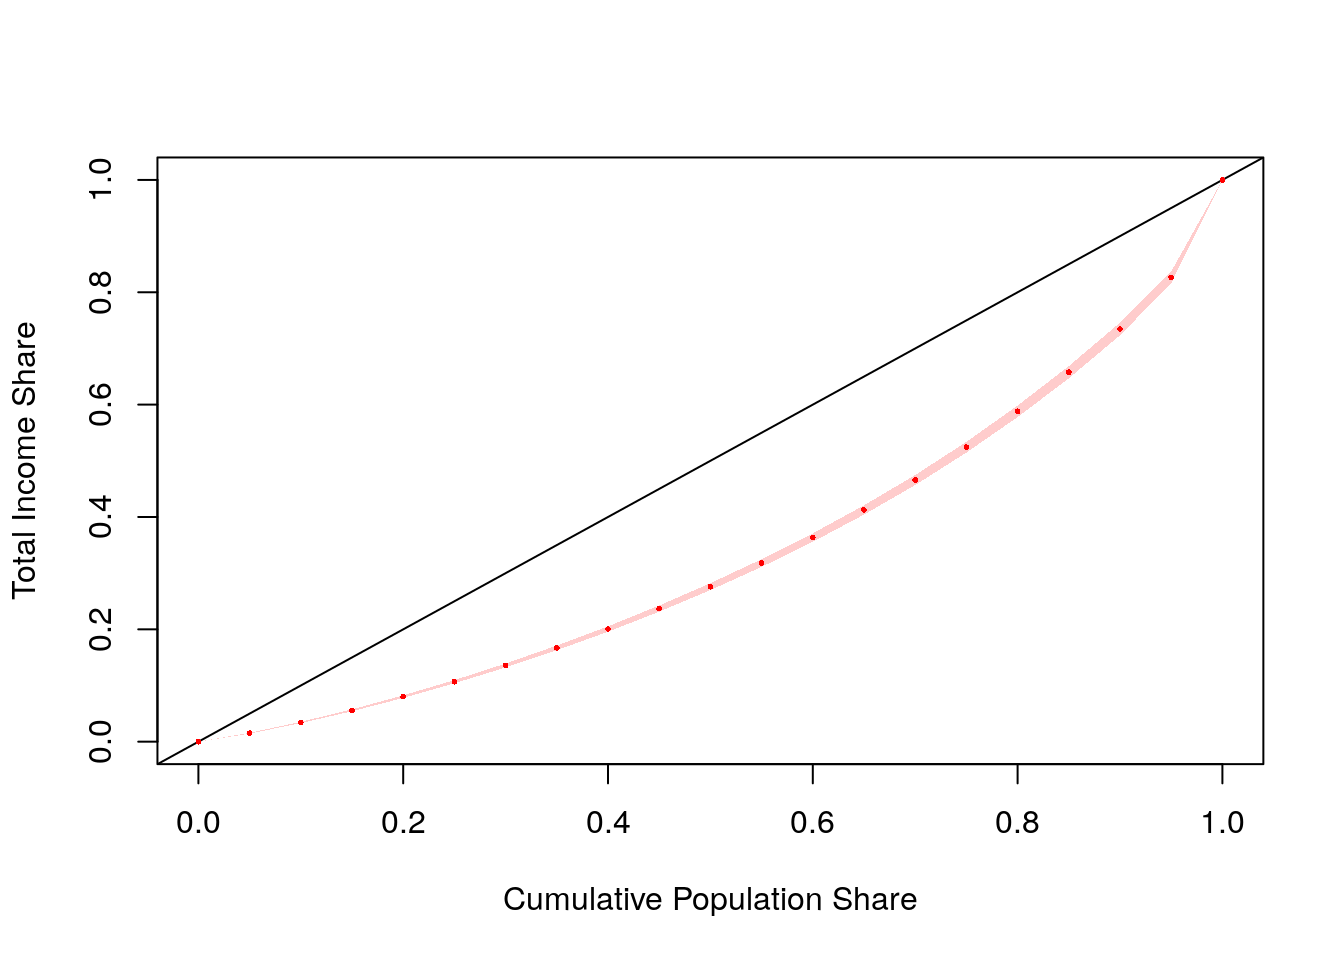
\includegraphics{context_files/figure-latex/unnamed-chunk-34-1.pdf}

\begin{Shaded}
\begin{Highlighting}[]
\CommentTok{\# note: most survey commands in R use Inf degrees of freedom by default}
\CommentTok{\# stata generally uses the degrees of freedom of the survey design.}
\CommentTok{\# therefore, while this extended syntax serves to prove a precise replication of stata}
\CommentTok{\# it is generally not necessary.}
\NormalTok{section\_four\_one }\OtherTok{\textless{}{-}}
	\FunctionTok{data.frame}\NormalTok{( }
		\AttributeTok{estimate =} \FunctionTok{coef}\NormalTok{( result.lin ) , }
		\AttributeTok{standard\_error =} \FunctionTok{SE}\NormalTok{( result.lin ) , }
		\AttributeTok{ci\_lower\_bound =} 
		    \FunctionTok{coef}\NormalTok{( result.lin ) }\SpecialCharTok{+} 
		    \FunctionTok{SE}\NormalTok{( result.lin ) }\SpecialCharTok{*} 
		    \FunctionTok{qt}\NormalTok{( }\FloatTok{0.025}\NormalTok{ , }\FunctionTok{degf}\NormalTok{( }\FunctionTok{subset}\NormalTok{( des\_nlsw88 , }\SpecialCharTok{!}\FunctionTok{is.na}\NormalTok{( wage ) ) ) ) ,}
		\AttributeTok{ci\_upper\_bound =} 
		    \FunctionTok{coef}\NormalTok{( result.lin ) }\SpecialCharTok{+} 
		    \FunctionTok{SE}\NormalTok{( result.lin ) }\SpecialCharTok{*} 
		    \FunctionTok{qt}\NormalTok{( }\FloatTok{0.975}\NormalTok{ , }\FunctionTok{degf}\NormalTok{( }\FunctionTok{subset}\NormalTok{( des\_nlsw88 , }\SpecialCharTok{!}\FunctionTok{is.na}\NormalTok{( wage ) ) ) )}
\NormalTok{	)}
\end{Highlighting}
\end{Shaded}

\begin{tabular}{lrrrr}
\toprule
  & estimate & standard\_error & ci\_lower\_bound & ci\_upper\_bound\\
\midrule
0 & 0.0000000 & 0.0000000 & 0.0000000 & 0.0000000\\
0.05 & 0.0151060 & 0.0004159 & 0.0142904 & 0.0159216\\
0.1 & 0.0342651 & 0.0007021 & 0.0328882 & 0.0356420\\
0.15 & 0.0558635 & 0.0010096 & 0.0538836 & 0.0578434\\
0.2 & 0.0801846 & 0.0014032 & 0.0774329 & 0.0829363\\
\addlinespace
0.25 & 0.1067687 & 0.0017315 & 0.1033732 & 0.1101642\\
0.3 & 0.1356307 & 0.0021301 & 0.1314535 & 0.1398078\\
0.35 & 0.1670287 & 0.0025182 & 0.1620903 & 0.1719670\\
0.4 & 0.2005501 & 0.0029161 & 0.1948315 & 0.2062687\\
0.45 & 0.2369209 & 0.0033267 & 0.2303971 & 0.2434447\\
\addlinespace
0.5 & 0.2759734 & 0.0037423 & 0.2686347 & 0.2833121\\
0.55 & 0.3180215 & 0.0041626 & 0.3098585 & 0.3261844\\
0.6 & 0.3633071 & 0.0045833 & 0.3543192 & 0.3722950\\
0.65 & 0.4125183 & 0.0050056 & 0.4027021 & 0.4223345\\
0.7 & 0.4657641 & 0.0054137 & 0.4551478 & 0.4763804\\
\addlinespace
0.75 & 0.5241784 & 0.0058003 & 0.5128039 & 0.5355529\\
0.8 & 0.5880894 & 0.0062464 & 0.5758401 & 0.6003388\\
0.85 & 0.6577051 & 0.0066148 & 0.6447333 & 0.6706769\\
0.9 & 0.7346412 & 0.0068289 & 0.7212497 & 0.7480328\\
0.95 & 0.8265786 & 0.0062686 & 0.8142857 & 0.8388715\\
\addlinespace
1 & 1.0000000 & 0.0000000 & 1.0000000 & 1.0000000\\
\bottomrule
\end{tabular}

For additional usage examples of \texttt{svylorenz}, type \texttt{?convey::svylorenz} in the R console.

\hypertarget{gini-index-svygini}{%
\section{Gini index (svygini)}\label{gini-index-svygini}}

The Gini index is an attempt to express the inequality presented in the Lorenz curve as a single number. In essence, it is twice the area between the equality curve and the real Lorenz curve. Put simply:

\[
\begin{aligned}
G &= 2 \bigg( \int_{0}^{1} pdp - \int_{0}^{1} L(p)dp \bigg) \\
\therefore G &= 1 - 2 \int_{0}^{1} L(p)dp
\end{aligned}
\]

where \(G=0\) in case of perfect equality and \(G = 1\) in the case of perfect inequality.

The estimator proposed by \citet{osier2009} is defined as:

\[
\widehat{G} = \frac{ 2 \sum_{i \in S} w_i r_i y_i - \sum_{i \in S} w_i y_i }{ \hat{Y} }
\]

The linearized formula of \(\widehat{G}\) is used to calculate the SE.

\begin{center}\rule{0.5\linewidth}{0.5pt}\end{center}

\textbf{A replication example}

The R \texttt{vardpoor} package \citep{vardpoor}, created by researchers at the Central Statistical Bureau of Latvia, includes a gini coefficient calculation using the ultimate cluster method. The example below reproduces those statistics.

Load and prepare the same data set:

\begin{Shaded}
\begin{Highlighting}[]
\CommentTok{\# load the convey package}
\FunctionTok{library}\NormalTok{(convey)}

\CommentTok{\# load the survey library}
\FunctionTok{library}\NormalTok{(survey)}

\CommentTok{\# load the vardpoor library}
\FunctionTok{library}\NormalTok{(vardpoor)}

\CommentTok{\# load the laeken library}
\FunctionTok{library}\NormalTok{(laeken)}

\CommentTok{\# load the synthetic EU statistics on income \& living conditions}
\FunctionTok{data}\NormalTok{(eusilc)}

\CommentTok{\# make all column names lowercase}
\FunctionTok{names}\NormalTok{( eusilc ) }\OtherTok{\textless{}{-}} \FunctionTok{tolower}\NormalTok{( }\FunctionTok{names}\NormalTok{( eusilc ) )}

\CommentTok{\# add a column with the row number}
\NormalTok{dati }\OtherTok{\textless{}{-}}\NormalTok{ data.table}\SpecialCharTok{::}\FunctionTok{data.table}\NormalTok{(}\AttributeTok{IDd =} \DecValTok{1} \SpecialCharTok{:} \FunctionTok{nrow}\NormalTok{(eusilc), eusilc)}

\CommentTok{\# calculate the gini coefficient}
\CommentTok{\# using the R vardpoor library}
\NormalTok{varpoord\_gini\_calculation }\OtherTok{\textless{}{-}}
	\FunctionTok{varpoord}\NormalTok{(}
	
		\CommentTok{\# analysis variable}
		\AttributeTok{Y =} \StringTok{"eqincome"}\NormalTok{, }
		
		\CommentTok{\# weights variable}
		\AttributeTok{w\_final =} \StringTok{"rb050"}\NormalTok{,}
		
		\CommentTok{\# row number variable}
		\AttributeTok{ID\_level1 =} \StringTok{"IDd"}\NormalTok{,}
		
		\CommentTok{\# row number variable}
		\AttributeTok{ID\_level2 =} \StringTok{"IDd"}\NormalTok{,}
		
		\CommentTok{\# strata variable}
		\AttributeTok{H =} \StringTok{"db040"}\NormalTok{, }
		
		\AttributeTok{N\_h =} \ConstantTok{NULL}\NormalTok{ ,}
		
		\CommentTok{\# clustering variable}
		\AttributeTok{PSU =} \StringTok{"rb030"}\NormalTok{, }
		
		\CommentTok{\# data.table}
		\AttributeTok{dataset =}\NormalTok{ dati, }
		
		\CommentTok{\# gini coefficient function}
		\AttributeTok{type =} \StringTok{"lingini"}\NormalTok{,}
	  
	  \CommentTok{\# poverty threshold range}
	  \AttributeTok{order\_quant =}\NormalTok{ 50L ,}
	  
	  \CommentTok{\# get linearized variable}
	  \AttributeTok{outp\_lin =} \ConstantTok{TRUE}
		
\NormalTok{	)}



\CommentTok{\# construct a survey.design}
\CommentTok{\# using our recommended setup}
\NormalTok{des\_eusilc }\OtherTok{\textless{}{-}} 
	\FunctionTok{svydesign}\NormalTok{( }
		\AttributeTok{ids =} \SpecialCharTok{\textasciitilde{}}\NormalTok{ rb030 , }
		\AttributeTok{strata =} \SpecialCharTok{\textasciitilde{}}\NormalTok{ db040 ,  }
		\AttributeTok{weights =} \SpecialCharTok{\textasciitilde{}}\NormalTok{ rb050 , }
		\AttributeTok{data =}\NormalTok{ eusilc}
\NormalTok{	)}

\CommentTok{\# immediately run the convey\_prep function on it}
\NormalTok{des\_eusilc }\OtherTok{\textless{}{-}} \FunctionTok{convey\_prep}\NormalTok{( des\_eusilc )}

\CommentTok{\# coefficients do match}
\NormalTok{varpoord\_gini\_calculation}\SpecialCharTok{$}\NormalTok{all\_result}\SpecialCharTok{$}\NormalTok{value}
\end{Highlighting}
\end{Shaded}

\begin{verbatim}
## [1] 26.49652
\end{verbatim}

\begin{Shaded}
\begin{Highlighting}[]
\FunctionTok{coef}\NormalTok{( }\FunctionTok{svygini}\NormalTok{( }\SpecialCharTok{\textasciitilde{}}\NormalTok{ eqincome , des\_eusilc ) ) }\SpecialCharTok{*} \DecValTok{100}
\end{Highlighting}
\end{Shaded}

\begin{verbatim}
## eqincome 
## 26.49652
\end{verbatim}

\begin{Shaded}
\begin{Highlighting}[]
\CommentTok{\# linearized variables do match}
\CommentTok{\# varpoord}
\NormalTok{lin\_gini\_varpoord}\OtherTok{\textless{}{-}}\NormalTok{ varpoord\_gini\_calculation}\SpecialCharTok{$}\NormalTok{lin\_out}\SpecialCharTok{$}\NormalTok{lin\_gini}
\CommentTok{\# convey }
\NormalTok{lin\_gini\_convey }\OtherTok{\textless{}{-}} \FunctionTok{attr}\NormalTok{(}\FunctionTok{svygini}\NormalTok{( }\SpecialCharTok{\textasciitilde{}}\NormalTok{ eqincome , des\_eusilc ),}\StringTok{"lin"}\NormalTok{)}

\CommentTok{\# check equality}
\FunctionTok{all.equal}\NormalTok{(lin\_gini\_varpoord,}\DecValTok{100}\SpecialCharTok{*}\NormalTok{lin\_gini\_convey )}
\end{Highlighting}
\end{Shaded}

\begin{verbatim}
## [1] TRUE
\end{verbatim}

\begin{Shaded}
\begin{Highlighting}[]
\CommentTok{\# variances do not match exactly}
\FunctionTok{attr}\NormalTok{( }\FunctionTok{svygini}\NormalTok{( }\SpecialCharTok{\textasciitilde{}}\NormalTok{ eqincome , des\_eusilc ) , }\StringTok{\textquotesingle{}var\textquotesingle{}}\NormalTok{ ) }\SpecialCharTok{*} \DecValTok{10000}
\end{Highlighting}
\end{Shaded}

\begin{verbatim}
##            eqincome
## eqincome 0.03790739
\end{verbatim}

\begin{Shaded}
\begin{Highlighting}[]
\NormalTok{varpoord\_gini\_calculation}\SpecialCharTok{$}\NormalTok{all\_result}\SpecialCharTok{$}\NormalTok{var}
\end{Highlighting}
\end{Shaded}

\begin{verbatim}
## [1] 0.03783931
\end{verbatim}

\begin{Shaded}
\begin{Highlighting}[]
\CommentTok{\# standard errors do not match exactly}
\NormalTok{varpoord\_gini\_calculation}\SpecialCharTok{$}\NormalTok{all\_result}\SpecialCharTok{$}\NormalTok{se}
\end{Highlighting}
\end{Shaded}

\begin{verbatim}
## [1] 0.1945233
\end{verbatim}

\begin{Shaded}
\begin{Highlighting}[]
\FunctionTok{SE}\NormalTok{( }\FunctionTok{svygini}\NormalTok{( }\SpecialCharTok{\textasciitilde{}}\NormalTok{ eqincome , des\_eusilc ) ) }\SpecialCharTok{*} \DecValTok{100}
\end{Highlighting}
\end{Shaded}

\begin{verbatim}
##           eqincome
## eqincome 0.1946982
\end{verbatim}

The variance estimate is computed by using the approximation defined in \eqref{eq:var}, where the linearized variable \(z\) is defined by \eqref{eq:lin}. The functions \texttt{convey::svygini} and \texttt{vardpoor::lingini} produce the same linearized variable \(z\).

However, the measures of uncertainty do not line up, because \texttt{library(vardpoor)} defaults to an ultimate cluster method that can be replicated with an alternative setup of the \texttt{survey.design} object.

\begin{Shaded}
\begin{Highlighting}[]
\CommentTok{\# within each strata, sum up the weights}
\NormalTok{cluster\_sums }\OtherTok{\textless{}{-}} \FunctionTok{aggregate}\NormalTok{( eusilc}\SpecialCharTok{$}\NormalTok{rb050 , }\FunctionTok{list}\NormalTok{( eusilc}\SpecialCharTok{$}\NormalTok{db040 ) , sum )}

\CommentTok{\# name the within{-}strata sums of weights the \textasciigrave{}cluster\_sum\textasciigrave{}}
\FunctionTok{names}\NormalTok{( cluster\_sums ) }\OtherTok{\textless{}{-}} \FunctionTok{c}\NormalTok{( }\StringTok{"db040"}\NormalTok{ , }\StringTok{"cluster\_sum"}\NormalTok{ )}

\CommentTok{\# merge this column back onto the data.frame}
\NormalTok{eusilc }\OtherTok{\textless{}{-}} \FunctionTok{merge}\NormalTok{( eusilc , cluster\_sums )}

\CommentTok{\# construct a survey.design}
\CommentTok{\# with the fpc using the cluster sum}
\NormalTok{des\_eusilc\_ultimate\_cluster }\OtherTok{\textless{}{-}} 
	\FunctionTok{svydesign}\NormalTok{( }
		\AttributeTok{ids =} \SpecialCharTok{\textasciitilde{}}\NormalTok{ rb030 , }
		\AttributeTok{strata =} \SpecialCharTok{\textasciitilde{}}\NormalTok{ db040 ,  }
		\AttributeTok{weights =} \SpecialCharTok{\textasciitilde{}}\NormalTok{ rb050 , }
		\AttributeTok{data =}\NormalTok{ eusilc , }
		\AttributeTok{fpc =} \SpecialCharTok{\textasciitilde{}}\NormalTok{ cluster\_sum }
\NormalTok{	)}

\CommentTok{\# again, immediately run the convey\_prep function on the \textasciigrave{}survey.design\textasciigrave{}}
\NormalTok{des\_eusilc\_ultimate\_cluster }\OtherTok{\textless{}{-}} \FunctionTok{convey\_prep}\NormalTok{( des\_eusilc\_ultimate\_cluster )}

\CommentTok{\# matches}
\FunctionTok{attr}\NormalTok{( }\FunctionTok{svygini}\NormalTok{( }\SpecialCharTok{\textasciitilde{}}\NormalTok{ eqincome , des\_eusilc\_ultimate\_cluster ) , }\StringTok{\textquotesingle{}var\textquotesingle{}}\NormalTok{ ) }\SpecialCharTok{*} \DecValTok{10000}
\end{Highlighting}
\end{Shaded}

\begin{verbatim}
##            eqincome
## eqincome 0.03783931
\end{verbatim}

\begin{Shaded}
\begin{Highlighting}[]
\NormalTok{varpoord\_gini\_calculation}\SpecialCharTok{$}\NormalTok{all\_result}\SpecialCharTok{$}\NormalTok{var}
\end{Highlighting}
\end{Shaded}

\begin{verbatim}
## [1] 0.03783931
\end{verbatim}

\begin{Shaded}
\begin{Highlighting}[]
\CommentTok{\# matches}
\NormalTok{varpoord\_gini\_calculation}\SpecialCharTok{$}\NormalTok{all\_result}\SpecialCharTok{$}\NormalTok{se}
\end{Highlighting}
\end{Shaded}

\begin{verbatim}
## [1] 0.1945233
\end{verbatim}

\begin{Shaded}
\begin{Highlighting}[]
\FunctionTok{SE}\NormalTok{( }\FunctionTok{svygini}\NormalTok{( }\SpecialCharTok{\textasciitilde{}}\NormalTok{ eqincome , des\_eusilc\_ultimate\_cluster ) ) }\SpecialCharTok{*} \DecValTok{100}
\end{Highlighting}
\end{Shaded}

\begin{verbatim}
##           eqincome
## eqincome 0.1945233
\end{verbatim}

\hypertarget{entropy-based-measures}{%
\section{Entropy-based Measures}\label{entropy-based-measures}}

Entropy is a concept derived from information theory, meaning the expected amount of information given the occurrence of an event. Following \citep{shannon1948}, given an event \(y\) with probability density function \(f(\cdot)\), the information content given the occurrence of \(y\) can be defined as \(g(f(y)) \colon= - \log f(y)\). Therefore, the expected information or, put simply, the \emph{entropy} is

\[
H(f) \colon = -E \big[ \log f(y) \big] = - \int_{-\infty}^{\infty} f(y) \log f(y) dy
\]

Assuming a discrete distribution, with \(p_k\) as the probability of occurring event \(k \in K\), the entropy formula takes the form:

\[
H = - \sum_{k \in K} p_k \log p_k \text{.}
\]

The main idea behind it is that the expected amount of information of an event is inversely proportional to the probability of its occurrence. In other words, the information derived from the observation of a rare event is higher than of the information of more probable events.

Using ideas presented in \citet{cowell2009}, substituting the density function by the income share of an individual \(s(q) = {F}^{-1}(q) / \int_{0}^{1} F^{-1}(t)dt = y/\mu\), the entropy function becomes the Theil\footnote{Also known as Theil-T index.} inequality index

\[
I_{Theil} = \int_{0}^{\infty} \frac{y}{\mu} \log \bigg( \frac{y}{\mu} \bigg) dF(y) = -H(s)
\]

Therefore, the entropy-based inequality measure increases as a person's income \(y\) deviates from the mean \(\mu\). This is the basic idea behind entropy-based inequality measures.

\hypertarget{generalized-entropy-and-decomposition-svygei-svygeidec}{%
\section{Generalized Entropy and Decomposition (svygei, svygeidec)}\label{generalized-entropy-and-decomposition-svygei-svygeidec}}

Using a generalization of the information function, now defined as \(g(f) = \frac{1}{\alpha-1} [ 1 - f^{\alpha - 1} ]\), the \(\alpha\)-class entropy is
\[
H_\alpha(f) = \frac{1}{\alpha - 1} \bigg[ 1 - \int_{-\infty}^{\infty} f(y)^{ \alpha - 1} f(y) dy \bigg] \text{.}
\]

This relates to a class of inequality measures, the Generalized entropy indices, defined as:

\[
GE_\alpha = \frac{1}{\alpha^2 - \alpha} \int_{0}^\infty \bigg[ \bigg( \frac{y}{\mu} \bigg)^\alpha - 1 \bigg]dF(x) = - \frac{-H_\alpha(s) }{ \alpha } \text{.}
\]

The parameter \(\alpha\) also has an economic interpretation: as \(\alpha\) increases, the influence of top incomes upon the index increases. In some cases, this measure takes special forms, such as mean log deviation and the aforementioned Theil index.

In order to estimate it, \citet{biewen2003} proposed the following:

\[
GE_\alpha =
\begin{cases}
( \alpha^2 - \alpha)^{-1} \big[ U_0^{\alpha - 1} U_1^{-\alpha} U_\alpha -1 \big], & \text{if } \alpha \in \mathbb{R} \setminus \{0,1\} \\
- T_0 U_0^{-1} + \log ( U_1 / U_0 ), &\text{if } \alpha \rightarrow 0 \\
T_1 U_1^{-1} - \log ( U_1 / U_0 ), & \text{if } \alpha \rightarrow 1
\end{cases}
\]

where \(U_\gamma = \sum_{i \in S} w_i \cdot y_i^\gamma\) and \(T_\gamma = \sum_{i \in S} w_i \cdot y_i^\gamma \cdot \log y_i\). Since those are all functions of totals, the linearization of the indices are easily achieved using the theorems described in \citet{deville1999}.

This class also has several desirable properties, such as additive decomposition. The additive decomposition allows to compare the effects of inequality within and between population groups on the population inequality. Put simply, an additive decomposable index allows for:

\[
I_{Total} = I_{Between} + I_{Within} \text{.}
\]

\begin{center}\rule{0.5\linewidth}{0.5pt}\end{center}

\textbf{A replication example}

In July 2006, \citet{jenkins2006} presented at the North American Stata Users' Group Meetings on the stata Generalized Entropy Index command. The example below reproduces those statistics.

Load and prepare the same data set:

\begin{Shaded}
\begin{Highlighting}[]
\CommentTok{\# load the convey package}
\FunctionTok{library}\NormalTok{(convey)}

\CommentTok{\# load the survey library}
\FunctionTok{library}\NormalTok{(survey)}

\CommentTok{\# load the foreign library}
\FunctionTok{library}\NormalTok{(foreign)}

\CommentTok{\# create a temporary file on the local disk}
\NormalTok{tf }\OtherTok{\textless{}{-}} \FunctionTok{tempfile}\NormalTok{()}

\CommentTok{\# store the location of the presentation file}
\NormalTok{presentation\_zip }\OtherTok{\textless{}{-}} \StringTok{"http://repec.org/nasug2006/nasug2006\_jenkins.zip"}

\CommentTok{\# download jenkins\textquotesingle{} presentation to the temporary file}
\FunctionTok{download.file}\NormalTok{( presentation\_zip , tf , }\AttributeTok{mode =} \StringTok{\textquotesingle{}wb\textquotesingle{}}\NormalTok{ )}

\CommentTok{\# unzip the contents of the archive}
\NormalTok{presentation\_files }\OtherTok{\textless{}{-}} \FunctionTok{unzip}\NormalTok{( tf , }\AttributeTok{exdir =} \FunctionTok{tempdir}\NormalTok{() )}

\CommentTok{\# load the institute for fiscal studies\textquotesingle{} 1981, 1985, and 1991 data.frame objects}
\NormalTok{x81 }\OtherTok{\textless{}{-}} \FunctionTok{read.dta}\NormalTok{( }\FunctionTok{grep}\NormalTok{( }\StringTok{"ifs81"}\NormalTok{ , presentation\_files , }\AttributeTok{value =} \ConstantTok{TRUE}\NormalTok{ ) )}
\NormalTok{x85 }\OtherTok{\textless{}{-}} \FunctionTok{read.dta}\NormalTok{( }\FunctionTok{grep}\NormalTok{( }\StringTok{"ifs85"}\NormalTok{ , presentation\_files , }\AttributeTok{value =} \ConstantTok{TRUE}\NormalTok{ ) )}
\NormalTok{x91 }\OtherTok{\textless{}{-}} \FunctionTok{read.dta}\NormalTok{( }\FunctionTok{grep}\NormalTok{( }\StringTok{"ifs91"}\NormalTok{ , presentation\_files , }\AttributeTok{value =} \ConstantTok{TRUE}\NormalTok{ ) )}

\CommentTok{\# stack each of these three years of data into a single data.frame}
\NormalTok{x }\OtherTok{\textless{}{-}} \FunctionTok{rbind}\NormalTok{( x81 , x85 , x91 )}
\end{Highlighting}
\end{Shaded}

Replicate the author's survey design statement from stata code..

\begin{verbatim}
. * account for clustering within HHs 
. version 8: svyset [pweight = wgt], psu(hrn)
pweight is wgt
psu is hrn
construct an
\end{verbatim}

.. into R code:

\begin{Shaded}
\begin{Highlighting}[]
\CommentTok{\# initiate a linearized survey design object}
\NormalTok{y }\OtherTok{\textless{}{-}} \FunctionTok{svydesign}\NormalTok{( }\SpecialCharTok{\textasciitilde{}}\NormalTok{ hrn , }\AttributeTok{data =}\NormalTok{ x , }\AttributeTok{weights =} \SpecialCharTok{\textasciitilde{}}\NormalTok{ wgt )}

\CommentTok{\# immediately run the \textasciigrave{}convey\_prep\textasciigrave{} function on the survey design}
\NormalTok{z }\OtherTok{\textless{}{-}} \FunctionTok{convey\_prep}\NormalTok{( y )}
\end{Highlighting}
\end{Shaded}

Replicate the author's subset statement and each of his svygei results..

\begin{verbatim}
. svygei x if year == 1981
 
Warning: x has 20 values = 0. Not used in calculations

Complex survey estimates of Generalized Entropy inequality indices
 
pweight: wgt                                   Number of obs    = 9752
Strata: <one>                                  Number of strata = 1
PSU: hrn                                       Number of PSUs   = 7459
											   Population size  = 54766261
---------------------------------------------------------------------------
Index    |  Estimate   Std. Err.      z      P>|z|     [95% Conf. Interval]
---------+-----------------------------------------------------------------
GE(-1)   |  .1902062   .02474921     7.69    0.000      .1416987   .2387138
MLD      |  .1142851   .00275138    41.54    0.000      .1088925   .1196777
Theil    |  .1116923   .00226489    49.31    0.000      .1072532   .1161314
GE(2)    |   .128793   .00330774    38.94    0.000      .1223099    .135276
GE(3)    |  .1739994   .00662015    26.28    0.000      .1610242   .1869747
---------------------------------------------------------------------------
\end{verbatim}

..using R code:

\begin{Shaded}
\begin{Highlighting}[]
\NormalTok{z81 }\OtherTok{\textless{}{-}} \FunctionTok{subset}\NormalTok{( z , year }\SpecialCharTok{==} \DecValTok{1981}\NormalTok{ )}

\FunctionTok{svygei}\NormalTok{( }\SpecialCharTok{\textasciitilde{}}\NormalTok{ eybhc0 , }\FunctionTok{subset}\NormalTok{( z81 , eybhc0 }\SpecialCharTok{\textgreater{}} \DecValTok{0}\NormalTok{ ) , }\AttributeTok{epsilon =} \SpecialCharTok{{-}}\DecValTok{1}\NormalTok{ )}
\end{Highlighting}
\end{Shaded}

\begin{verbatim}
##             gei       SE epsilon
## eybhc0 0.190206 0.024748      -1
\end{verbatim}

\begin{Shaded}
\begin{Highlighting}[]
\FunctionTok{svygei}\NormalTok{( }\SpecialCharTok{\textasciitilde{}}\NormalTok{ eybhc0 , }\FunctionTok{subset}\NormalTok{( z81 , eybhc0 }\SpecialCharTok{\textgreater{}} \DecValTok{0}\NormalTok{ ) , }\AttributeTok{epsilon =} \DecValTok{0}\NormalTok{ )}
\end{Highlighting}
\end{Shaded}

\begin{verbatim}
##              gei        SE epsilon
## eybhc0 0.1142851 0.0027513       0
\end{verbatim}

\begin{Shaded}
\begin{Highlighting}[]
\FunctionTok{svygei}\NormalTok{( }\SpecialCharTok{\textasciitilde{}}\NormalTok{ eybhc0 , }\FunctionTok{subset}\NormalTok{( z81 , eybhc0 }\SpecialCharTok{\textgreater{}} \DecValTok{0}\NormalTok{ ) )}
\end{Highlighting}
\end{Shaded}

\begin{verbatim}
##              gei        SE epsilon
## eybhc0 0.1116923 0.0022648       1
\end{verbatim}

\begin{Shaded}
\begin{Highlighting}[]
\FunctionTok{svygei}\NormalTok{( }\SpecialCharTok{\textasciitilde{}}\NormalTok{ eybhc0 , }\FunctionTok{subset}\NormalTok{( z81 , eybhc0 }\SpecialCharTok{\textgreater{}} \DecValTok{0}\NormalTok{ ) , }\AttributeTok{epsilon =} \DecValTok{2}\NormalTok{ )}
\end{Highlighting}
\end{Shaded}

\begin{verbatim}
##              gei        SE epsilon
## eybhc0 0.1287930 0.0033076       2
\end{verbatim}

\begin{Shaded}
\begin{Highlighting}[]
\FunctionTok{svygei}\NormalTok{( }\SpecialCharTok{\textasciitilde{}}\NormalTok{ eybhc0 , }\FunctionTok{subset}\NormalTok{( z81 , eybhc0 }\SpecialCharTok{\textgreater{}} \DecValTok{0}\NormalTok{ ) , }\AttributeTok{epsilon =} \DecValTok{3}\NormalTok{ )}
\end{Highlighting}
\end{Shaded}

\begin{verbatim}
##              gei        SE epsilon
## eybhc0 0.1739994 0.0066199       3
\end{verbatim}

Confirm this replication applies for subsetted objects as well. Compare stata output..

\begin{verbatim}
. svygei x if year == 1985 & x >= 1

Complex survey estimates of Generalized Entropy inequality indices
 
pweight: wgt                                   Number of obs    = 8969
Strata: <one>                                  Number of strata = 1
PSU: hrn                                       Number of PSUs   = 6950
											   Population size  = 55042871
---------------------------------------------------------------------------
Index    |  Estimate   Std. Err.      z      P>|z|     [95% Conf. Interval]
---------+-----------------------------------------------------------------
GE(-1)   |  .1602358   .00936931    17.10    0.000      .1418723   .1785993
MLD      |   .127616   .00332187    38.42    0.000      .1211052   .1341267
Theil    |  .1337177   .00406302    32.91    0.000      .1257543    .141681
GE(2)    |  .1676393   .00730057    22.96    0.000      .1533304   .1819481
GE(3)    |  .2609507   .01850689    14.10    0.000      .2246779   .2972235
---------------------------------------------------------------------------
\end{verbatim}

..to R code:

\begin{Shaded}
\begin{Highlighting}[]
\NormalTok{z85 }\OtherTok{\textless{}{-}} \FunctionTok{subset}\NormalTok{( z , year }\SpecialCharTok{==} \DecValTok{1985}\NormalTok{ )}

\FunctionTok{svygei}\NormalTok{( }\SpecialCharTok{\textasciitilde{}}\NormalTok{ eybhc0 , }\FunctionTok{subset}\NormalTok{( z85 , eybhc0 }\SpecialCharTok{\textgreater{}} \DecValTok{1}\NormalTok{ ) , }\AttributeTok{epsilon =} \SpecialCharTok{{-}}\DecValTok{1}\NormalTok{ )}
\end{Highlighting}
\end{Shaded}

\begin{verbatim}
##              gei        SE epsilon
## eybhc0 0.1602358 0.0093689      -1
\end{verbatim}

\begin{Shaded}
\begin{Highlighting}[]
\FunctionTok{svygei}\NormalTok{( }\SpecialCharTok{\textasciitilde{}}\NormalTok{ eybhc0 , }\FunctionTok{subset}\NormalTok{( z85 , eybhc0 }\SpecialCharTok{\textgreater{}} \DecValTok{1}\NormalTok{ ) , }\AttributeTok{epsilon =} \DecValTok{0}\NormalTok{ )}
\end{Highlighting}
\end{Shaded}

\begin{verbatim}
##              gei        SE epsilon
## eybhc0 0.1276160 0.0033217       0
\end{verbatim}

\begin{Shaded}
\begin{Highlighting}[]
\FunctionTok{svygei}\NormalTok{( }\SpecialCharTok{\textasciitilde{}}\NormalTok{ eybhc0 , }\FunctionTok{subset}\NormalTok{( z85 , eybhc0 }\SpecialCharTok{\textgreater{}} \DecValTok{1}\NormalTok{ ) )}
\end{Highlighting}
\end{Shaded}

\begin{verbatim}
##              gei        SE epsilon
## eybhc0 0.1337177 0.0040628       1
\end{verbatim}

\begin{Shaded}
\begin{Highlighting}[]
\FunctionTok{svygei}\NormalTok{( }\SpecialCharTok{\textasciitilde{}}\NormalTok{ eybhc0 , }\FunctionTok{subset}\NormalTok{( z85 , eybhc0 }\SpecialCharTok{\textgreater{}} \DecValTok{1}\NormalTok{ ) , }\AttributeTok{epsilon =} \DecValTok{2}\NormalTok{ )}
\end{Highlighting}
\end{Shaded}

\begin{verbatim}
##              gei        SE epsilon
## eybhc0 0.1676393 0.0073002       2
\end{verbatim}

\begin{Shaded}
\begin{Highlighting}[]
\FunctionTok{svygei}\NormalTok{( }\SpecialCharTok{\textasciitilde{}}\NormalTok{ eybhc0 , }\FunctionTok{subset}\NormalTok{( z85 , eybhc0 }\SpecialCharTok{\textgreater{}} \DecValTok{1}\NormalTok{ ) , }\AttributeTok{epsilon =} \DecValTok{3}\NormalTok{ )}
\end{Highlighting}
\end{Shaded}

\begin{verbatim}
##             gei       SE epsilon
## eybhc0 0.260951 0.018506       3
\end{verbatim}

Replicate the author's decomposition by population subgroup (work status) shown on PDF page 57..

\begin{Shaded}
\begin{Highlighting}[]
\CommentTok{\# define work status (PDF page 22)}
\NormalTok{z }\OtherTok{\textless{}{-}} \FunctionTok{update}\NormalTok{( z , }\AttributeTok{wkstatus =} \FunctionTok{c}\NormalTok{( }\DecValTok{1}\NormalTok{ , }\DecValTok{1}\NormalTok{ , }\DecValTok{1}\NormalTok{ , }\DecValTok{1}\NormalTok{ , }\DecValTok{2}\NormalTok{ , }\DecValTok{3}\NormalTok{ , }\DecValTok{2}\NormalTok{ , }\DecValTok{2}\NormalTok{ )[ }\FunctionTok{as.numeric}\NormalTok{( esbu ) ] )}
\NormalTok{z }\OtherTok{\textless{}{-}} \FunctionTok{update}\NormalTok{( z , }\FunctionTok{factor}\NormalTok{( wkstatus , }\AttributeTok{labels =} \FunctionTok{c}\NormalTok{( }\StringTok{"1+ ft working"}\NormalTok{ , }\StringTok{"no ft working"}\NormalTok{ , }\StringTok{"elderly"}\NormalTok{ ) ) )}

\CommentTok{\# subset to 1991 and remove records with zero income}
\NormalTok{z91 }\OtherTok{\textless{}{-}} \FunctionTok{subset}\NormalTok{( z , year }\SpecialCharTok{==} \DecValTok{1991} \SpecialCharTok{\&}\NormalTok{ eybhc0 }\SpecialCharTok{\textgreater{}} \DecValTok{0}\NormalTok{ )}

\CommentTok{\# population share}
\FunctionTok{svymean}\NormalTok{( }\SpecialCharTok{\textasciitilde{}}\NormalTok{wkstatus, z91 )}
\end{Highlighting}
\end{Shaded}

\begin{verbatim}
##            mean     SE
## wkstatus 1.5594 0.0099
\end{verbatim}

\begin{Shaded}
\begin{Highlighting}[]
\CommentTok{\# mean}
\FunctionTok{svyby}\NormalTok{( }\SpecialCharTok{\textasciitilde{}}\NormalTok{eybhc0, }\SpecialCharTok{\textasciitilde{}}\NormalTok{wkstatus, z91, svymean )}
\end{Highlighting}
\end{Shaded}

\begin{verbatim}
##   wkstatus   eybhc0       se
## 1        1 278.8040 3.703790
## 2        2 151.6317 3.153968
## 3        3 176.6045 4.661740
\end{verbatim}

\begin{Shaded}
\begin{Highlighting}[]
\CommentTok{\# subgroup indices: ge\_k}
\FunctionTok{svyby}\NormalTok{( }\SpecialCharTok{\textasciitilde{}}\NormalTok{ eybhc0 , }\SpecialCharTok{\textasciitilde{}}\NormalTok{wkstatus , z91 , svygei , }\AttributeTok{epsilon =} \SpecialCharTok{{-}}\DecValTok{1}\NormalTok{ )}
\end{Highlighting}
\end{Shaded}

\begin{verbatim}
##   wkstatus     eybhc0          se
## 1        1  0.2300708  0.02853959
## 2        2 10.9231761 10.65482557
## 3        3  0.1932164  0.02571991
\end{verbatim}

\begin{Shaded}
\begin{Highlighting}[]
\FunctionTok{svyby}\NormalTok{( }\SpecialCharTok{\textasciitilde{}}\NormalTok{ eybhc0 , }\SpecialCharTok{\textasciitilde{}}\NormalTok{wkstatus , z91 , svygei , }\AttributeTok{epsilon =} \DecValTok{0}\NormalTok{ )}
\end{Highlighting}
\end{Shaded}

\begin{verbatim}
##   wkstatus    eybhc0          se
## 1        1 0.1536921 0.006955506
## 2        2 0.1836835 0.014740510
## 3        3 0.1653658 0.016409770
\end{verbatim}

\begin{Shaded}
\begin{Highlighting}[]
\FunctionTok{svyby}\NormalTok{( }\SpecialCharTok{\textasciitilde{}}\NormalTok{ eybhc0 , }\SpecialCharTok{\textasciitilde{}}\NormalTok{wkstatus , z91 , svygei , }\AttributeTok{epsilon =} \DecValTok{1}\NormalTok{ )}
\end{Highlighting}
\end{Shaded}

\begin{verbatim}
##   wkstatus    eybhc0          se
## 1        1 0.1598558 0.008327994
## 2        2 0.1889909 0.016766120
## 3        3 0.2023862 0.027787224
\end{verbatim}

\begin{Shaded}
\begin{Highlighting}[]
\FunctionTok{svyby}\NormalTok{( }\SpecialCharTok{\textasciitilde{}}\NormalTok{ eybhc0 , }\SpecialCharTok{\textasciitilde{}}\NormalTok{wkstatus , z91 , svygei , }\AttributeTok{epsilon =} \DecValTok{2}\NormalTok{ )}
\end{Highlighting}
\end{Shaded}

\begin{verbatim}
##   wkstatus    eybhc0         se
## 1        1 0.2130664 0.01546521
## 2        2 0.2846345 0.06016394
## 3        3 0.3465088 0.07362898
\end{verbatim}

\begin{Shaded}
\begin{Highlighting}[]
\CommentTok{\# GE decomposition}
\FunctionTok{svygeidec}\NormalTok{( }\SpecialCharTok{\textasciitilde{}}\NormalTok{eybhc0, }\SpecialCharTok{\textasciitilde{}}\NormalTok{wkstatus, z91, }\AttributeTok{epsilon =} \SpecialCharTok{{-}}\DecValTok{1}\NormalTok{ )}
\end{Highlighting}
\end{Shaded}

\begin{verbatim}
##       total within between
## coef 3.6829 3.6466  0.0363
## SE   3.3999 3.3993  0.0541
\end{verbatim}

\begin{Shaded}
\begin{Highlighting}[]
\FunctionTok{svygeidec}\NormalTok{( }\SpecialCharTok{\textasciitilde{}}\NormalTok{eybhc0, }\SpecialCharTok{\textasciitilde{}}\NormalTok{wkstatus, z91, }\AttributeTok{epsilon =} \DecValTok{0}\NormalTok{ )}
\end{Highlighting}
\end{Shaded}

\begin{verbatim}
##          total    within between
## coef 0.1952363 0.1619352  0.0333
## SE   0.0064615 0.0062209  0.0027
\end{verbatim}

\begin{Shaded}
\begin{Highlighting}[]
\FunctionTok{svygeidec}\NormalTok{( }\SpecialCharTok{\textasciitilde{}}\NormalTok{eybhc0, }\SpecialCharTok{\textasciitilde{}}\NormalTok{wkstatus, z91, }\AttributeTok{epsilon =} \DecValTok{1}\NormalTok{ )}
\end{Highlighting}
\end{Shaded}

\begin{verbatim}
##          total    within between
## coef 0.2003897 0.1693958  0.0310
## SE   0.0079299 0.0082236  0.0027
\end{verbatim}

\begin{Shaded}
\begin{Highlighting}[]
\FunctionTok{svygeidec}\NormalTok{( }\SpecialCharTok{\textasciitilde{}}\NormalTok{eybhc0, }\SpecialCharTok{\textasciitilde{}}\NormalTok{wkstatus, z91, }\AttributeTok{epsilon =} \DecValTok{2}\NormalTok{ )}
\end{Highlighting}
\end{Shaded}

\begin{verbatim}
##         total   within between
## coef 0.274325 0.245067  0.0293
## SE   0.016694 0.017831  0.0038
\end{verbatim}

For additional usage examples of \texttt{svygei} or \texttt{svygeidec}, type \texttt{?convey::svygei} or \texttt{?convey::svygeidec} in the R console.

\hypertarget{j-divergence-and-decomposition-svyjdiv-svyjdivdec}{%
\section{J-Divergence and Decomposition (svyjdiv, svyjdivdec)}\label{j-divergence-and-decomposition-svyjdiv-svyjdivdec}}

The J-divergence measure \citep{rohde2016} can be seen as the sum of \(GE_0\) and \(GE_1\), satisfying axioms that, individually, those two indices do not. Using \(U_\gamma\) and \(T_\gamma\) functions defined in \citet{biewen2003}, the estimator can be defined as:

\[
\begin{aligned}
J &= \frac{1}{N} \sum_{i \in S} \bigg( \frac{ y_i - \mu }{ \mu } \bigg) \log \bigg( \frac{y_i}{\mu} \bigg) \\
\therefore \widehat{J} &= \frac{\widehat{T}_1}{\widehat{U}_1} - \frac{ \widehat{T}_0 }{ \widehat{U}_0 }
\end{aligned}
\]

Since it is a sum of two additive decomposable measures, \(J\) itself is decomposable.

For additional usage examples of \texttt{svyjdiv} or \texttt{svyjdivdec}, type \texttt{?convey::svyjdiv} or \texttt{?convey::svyjdivdec} in the R console.

\hypertarget{atkinson-index-svyatk}{%
\section{Atkinson index (svyatk)}\label{atkinson-index-svyatk}}

Although the original formula was proposed in \citet{atkinson1970}, the estimator used here comes from \citet{biewen2003}:

\[
\widehat{A}_\epsilon =
\begin{cases}
 1 - \widehat{U}_0^{ - \epsilon/(1 - \epsilon) } \widehat{U}_1^{ -1 } \widehat{U}_{1 - \epsilon}^{ 1/(1 - \epsilon) } , &\text{if } \epsilon \in \mathbb{R}_+ \setminus\{ 1 \} \\
1 - \widehat{U}_0 \widehat{U}_0^{-1} exp( \widehat{T}_0 \widehat{U}_0^{-1} ), &\text{if } \epsilon \rightarrow1
\end{cases}
\]

The \(\epsilon\) is an inequality aversion parameter: as it approaches infinity, more weight is given to incomes in bottom of the distribution.

\begin{center}\rule{0.5\linewidth}{0.5pt}\end{center}

\textbf{A replication example}

In July 2006, \citet{jenkins2006} presented at the North American Stata Users' Group Meetings on the stata Atkinson Index command. The example below reproduces those statistics.

Load and prepare the same data set:

\begin{Shaded}
\begin{Highlighting}[]
\CommentTok{\# load the convey package}
\FunctionTok{library}\NormalTok{(convey)}

\CommentTok{\# load the survey library}
\FunctionTok{library}\NormalTok{(survey)}

\CommentTok{\# load the foreign library}
\FunctionTok{library}\NormalTok{(foreign)}

\CommentTok{\# create a temporary file on the local disk}
\NormalTok{tf }\OtherTok{\textless{}{-}} \FunctionTok{tempfile}\NormalTok{()}

\CommentTok{\# store the location of the presentation file}
\NormalTok{presentation\_zip }\OtherTok{\textless{}{-}} \StringTok{"http://repec.org/nasug2006/nasug2006\_jenkins.zip"}

\CommentTok{\# download jenkins\textquotesingle{} presentation to the temporary file}
\FunctionTok{download.file}\NormalTok{( presentation\_zip , tf , }\AttributeTok{mode =} \StringTok{\textquotesingle{}wb\textquotesingle{}}\NormalTok{ )}

\CommentTok{\# unzip the contents of the archive}
\NormalTok{presentation\_files }\OtherTok{\textless{}{-}} \FunctionTok{unzip}\NormalTok{( tf , }\AttributeTok{exdir =} \FunctionTok{tempdir}\NormalTok{() )}

\CommentTok{\# load the institute for fiscal studies\textquotesingle{} 1981, 1985, and 1991 data.frame objects}
\NormalTok{x81 }\OtherTok{\textless{}{-}} \FunctionTok{read.dta}\NormalTok{( }\FunctionTok{grep}\NormalTok{( }\StringTok{"ifs81"}\NormalTok{ , presentation\_files , }\AttributeTok{value =} \ConstantTok{TRUE}\NormalTok{ ) )}
\NormalTok{x85 }\OtherTok{\textless{}{-}} \FunctionTok{read.dta}\NormalTok{( }\FunctionTok{grep}\NormalTok{( }\StringTok{"ifs85"}\NormalTok{ , presentation\_files , }\AttributeTok{value =} \ConstantTok{TRUE}\NormalTok{ ) )}
\NormalTok{x91 }\OtherTok{\textless{}{-}} \FunctionTok{read.dta}\NormalTok{( }\FunctionTok{grep}\NormalTok{( }\StringTok{"ifs91"}\NormalTok{ , presentation\_files , }\AttributeTok{value =} \ConstantTok{TRUE}\NormalTok{ ) )}

\CommentTok{\# stack each of these three years of data into a single data.frame}
\NormalTok{x }\OtherTok{\textless{}{-}} \FunctionTok{rbind}\NormalTok{( x81 , x85 , x91 )}
\end{Highlighting}
\end{Shaded}

Replicate the author's survey design statement from stata code..

\begin{verbatim}
. * account for clustering within HHs 
. version 8: svyset [pweight = wgt], psu(hrn)
pweight is wgt
psu is hrn
construct an
\end{verbatim}

.. into R code:

\begin{Shaded}
\begin{Highlighting}[]
\CommentTok{\# initiate a linearized survey design object}
\NormalTok{y }\OtherTok{\textless{}{-}} \FunctionTok{svydesign}\NormalTok{( }\SpecialCharTok{\textasciitilde{}}\NormalTok{ hrn , }\AttributeTok{data =}\NormalTok{ x , }\AttributeTok{weights =} \SpecialCharTok{\textasciitilde{}}\NormalTok{ wgt )}

\CommentTok{\# immediately run the \textasciigrave{}convey\_prep\textasciigrave{} function on the survey design}
\NormalTok{z }\OtherTok{\textless{}{-}} \FunctionTok{convey\_prep}\NormalTok{( y )}
\end{Highlighting}
\end{Shaded}

Replicate the author's subset statement and each of his svyatk results with stata..

\begin{verbatim}
. svyatk x if year == 1981
 
Warning: x has 20 values = 0. Not used in calculations

Complex survey estimates of Atkinson inequality indices
 
pweight: wgt                                   Number of obs    = 9752
Strata: <one>                                  Number of strata = 1
PSU: hrn                                       Number of PSUs   = 7459
                                               Population size  = 54766261
---------------------------------------------------------------------------
Index    |  Estimate   Std. Err.      z      P>|z|     [95% Conf. Interval]
---------+-----------------------------------------------------------------
A(0.5)   |  .0543239   .00107583    50.49    0.000      .0522153   .0564324
A(1)     |  .1079964   .00245424    44.00    0.000      .1031862   .1128066
A(1.5)   |  .1701794   .0066943    25.42    0.000       .1570588      .1833
A(2)     |  .2755788   .02597608    10.61    0.000      .2246666    .326491
A(2.5)   |  .4992701   .06754311     7.39    0.000       .366888   .6316522
---------------------------------------------------------------------------
\end{verbatim}

..using R code:

\begin{Shaded}
\begin{Highlighting}[]
\NormalTok{z81 }\OtherTok{\textless{}{-}} \FunctionTok{subset}\NormalTok{( z , year }\SpecialCharTok{==} \DecValTok{1981}\NormalTok{ )}

\FunctionTok{svyatk}\NormalTok{( }\SpecialCharTok{\textasciitilde{}}\NormalTok{ eybhc0 , }\FunctionTok{subset}\NormalTok{( z81 , eybhc0 }\SpecialCharTok{\textgreater{}} \DecValTok{0}\NormalTok{ ) , }\AttributeTok{epsilon =} \FloatTok{0.5}\NormalTok{ )}
\end{Highlighting}
\end{Shaded}

\begin{verbatim}
##        atkinson     SE
## eybhc0 0.054324 0.0011
\end{verbatim}

\begin{Shaded}
\begin{Highlighting}[]
\FunctionTok{svyatk}\NormalTok{( }\SpecialCharTok{\textasciitilde{}}\NormalTok{ eybhc0 , }\FunctionTok{subset}\NormalTok{( z81 , eybhc0 }\SpecialCharTok{\textgreater{}} \DecValTok{0}\NormalTok{ ) )}
\end{Highlighting}
\end{Shaded}

\begin{verbatim}
##        atkinson     SE
## eybhc0    0.108 0.0025
\end{verbatim}

\begin{Shaded}
\begin{Highlighting}[]
\FunctionTok{svyatk}\NormalTok{( }\SpecialCharTok{\textasciitilde{}}\NormalTok{ eybhc0 , }\FunctionTok{subset}\NormalTok{( z81 , eybhc0 }\SpecialCharTok{\textgreater{}} \DecValTok{0}\NormalTok{ ) , }\AttributeTok{epsilon =} \FloatTok{1.5}\NormalTok{ )}
\end{Highlighting}
\end{Shaded}

\begin{verbatim}
##        atkinson     SE
## eybhc0  0.17018 0.0067
\end{verbatim}

\begin{Shaded}
\begin{Highlighting}[]
\FunctionTok{svyatk}\NormalTok{( }\SpecialCharTok{\textasciitilde{}}\NormalTok{ eybhc0 , }\FunctionTok{subset}\NormalTok{( z81 , eybhc0 }\SpecialCharTok{\textgreater{}} \DecValTok{0}\NormalTok{ ) , }\AttributeTok{epsilon =} \DecValTok{2}\NormalTok{ )}
\end{Highlighting}
\end{Shaded}

\begin{verbatim}
##        atkinson    SE
## eybhc0  0.27558 0.026
\end{verbatim}

\begin{Shaded}
\begin{Highlighting}[]
\FunctionTok{svyatk}\NormalTok{( }\SpecialCharTok{\textasciitilde{}}\NormalTok{ eybhc0 , }\FunctionTok{subset}\NormalTok{( z81 , eybhc0 }\SpecialCharTok{\textgreater{}} \DecValTok{0}\NormalTok{ ) , }\AttributeTok{epsilon =} \FloatTok{2.5}\NormalTok{ )}
\end{Highlighting}
\end{Shaded}

\begin{verbatim}
##        atkinson     SE
## eybhc0  0.49927 0.0675
\end{verbatim}

Confirm this replication applies for subsetted objects as well, comparing stata code..

\begin{verbatim}
. svyatk x if year == 1981 & x >= 1

Complex survey estimates of Atkinson inequality indices
 
pweight: wgt                                   Number of obs    = 9748
Strata: <one>                                  Number of strata = 1
PSU: hrn                                       Number of PSUs   = 7457
                                               Population size  = 54744234
---------------------------------------------------------------------------
Index    |  Estimate   Std. Err.      z      P>|z|     [95% Conf. Interval]
---------+-----------------------------------------------------------------
A(0.5)   |  .0540059   .00105011    51.43    0.000      .0519477   .0560641
A(1)     |  .1066082   .00223318    47.74    0.000      .1022313   .1109852
A(1.5)   |  .1638299   .00483069    33.91    0.000       .154362   .1732979
A(2)     |  .2443206   .01425258    17.14    0.000      .2163861   .2722552
A(2.5)   |   .394787   .04155221     9.50    0.000      .3133461   .4762278
---------------------------------------------------------------------------
\end{verbatim}

..to R code:

\begin{Shaded}
\begin{Highlighting}[]
\NormalTok{z81\_two }\OtherTok{\textless{}{-}} \FunctionTok{subset}\NormalTok{( z , year }\SpecialCharTok{==} \DecValTok{1981} \SpecialCharTok{\&}\NormalTok{ eybhc0 }\SpecialCharTok{\textgreater{}} \DecValTok{1}\NormalTok{ )}

\FunctionTok{svyatk}\NormalTok{( }\SpecialCharTok{\textasciitilde{}}\NormalTok{ eybhc0 , z81\_two , }\AttributeTok{epsilon =} \FloatTok{0.5}\NormalTok{ )}
\end{Highlighting}
\end{Shaded}

\begin{verbatim}
##        atkinson     SE
## eybhc0 0.054006 0.0011
\end{verbatim}

\begin{Shaded}
\begin{Highlighting}[]
\FunctionTok{svyatk}\NormalTok{( }\SpecialCharTok{\textasciitilde{}}\NormalTok{ eybhc0 , z81\_two )}
\end{Highlighting}
\end{Shaded}

\begin{verbatim}
##        atkinson     SE
## eybhc0  0.10661 0.0022
\end{verbatim}

\begin{Shaded}
\begin{Highlighting}[]
\FunctionTok{svyatk}\NormalTok{( }\SpecialCharTok{\textasciitilde{}}\NormalTok{ eybhc0 , z81\_two , }\AttributeTok{epsilon =} \FloatTok{1.5}\NormalTok{ )}
\end{Highlighting}
\end{Shaded}

\begin{verbatim}
##        atkinson     SE
## eybhc0  0.16383 0.0048
\end{verbatim}

\begin{Shaded}
\begin{Highlighting}[]
\FunctionTok{svyatk}\NormalTok{( }\SpecialCharTok{\textasciitilde{}}\NormalTok{ eybhc0 , z81\_two , }\AttributeTok{epsilon =} \DecValTok{2}\NormalTok{ )}
\end{Highlighting}
\end{Shaded}

\begin{verbatim}
##        atkinson     SE
## eybhc0  0.24432 0.0143
\end{verbatim}

\begin{Shaded}
\begin{Highlighting}[]
\FunctionTok{svyatk}\NormalTok{( }\SpecialCharTok{\textasciitilde{}}\NormalTok{ eybhc0 , z81\_two , }\AttributeTok{epsilon =} \FloatTok{2.5}\NormalTok{ )}
\end{Highlighting}
\end{Shaded}

\begin{verbatim}
##        atkinson     SE
## eybhc0  0.39479 0.0416
\end{verbatim}

For additional usage examples of \texttt{svyatk}, type \texttt{?convey::svyatk} in the R console.

\hypertarget{which-inequality-measure-should-be-used}{%
\section{Which inequality measure should be used?}\label{which-inequality-measure-should-be-used}}

The variety of inequality measures begs a question: which inequality measure shuold be used? In fact, this is a very important question. However, the nature of it is not statistical or mathematical, but ethical. This section aims to clarify and, while not proposing a ``perfect measure'', to provide the reader with an initial guidance about which measure to use.

The most general way to analyze if one distribution is more equally distributed than another is by the Lorenz curve. When \(L_A(p) \geqslant L_B(p), \forall p \in [0,1]\), it is said that \(A\) is more equally distributed than \(B\). Technically, we say that \(A\) \emph{(Lorenz )dominates} \(B\)\footnote{\citet{kramer1998} and \citet{mosler1994} provide helpful insights to how majorization, Lorenz dominance, and inequality measurement are connected. On the topic of majorization, \citet{hardy1934} is still the main reference, while \citet{olkin2011} provide a more modern approach.}. In this case, all inequality measures that satisfy basic properties\footnote{Namely, Schur-convexity, population invariance, and scale invariance.} will agree that \(A\) is more equally distributed than \(B\).

When this dominance fails, i.e., when Lorenz curves do cross, Lorenz ordering is impossible. Then, under such circumstances, the choice of which inequality measure to use becomes relevant.

Each inequality measure is a result of a subjective understanding of what is a fair distribution. As \citet[p.348]{dalton1920} puts it, ``{[}\ldots{]} the economist is primarily interested, not in the distribution of income as such, but in the effects of the distribution of income upon the distribution and total amount of economic welfare, which may be derived from income.'' The importance of how economic welfare is defined is once again expressed by \citet{atkinson1970}, where an inequality measure is direclty derived from a class of welfare functions. Even when a welfare function is not explicit, such as in the Gini index, we must agree that an implicit, subjective judgement of the impact of inequality on social welfare is assumed.

The idea of what is a fair distribution is a matter of Ethics, a discipline within the realm of Philosophy. Yet, as \citet[Ch.1]{fleur1996} proposes, the analyst should match socially supported moral values and theories of justice to the set of technical tools for policy evaluation.

Although this can be a useful principle, a more objective answer is needed. By knowing the nature and properties of inequality measures, the analyst can further reduce the set of applicable inequality measures. For instance, choosing from the properties listed in \citet[p.74]{cowell2011}, if we require group-decomposability, scale invariance, population invariance, and that the estimate in \([0,1]\), we must resort to the Atkinson index.

Even though the discussion can go deep in technical and philosophical aspects, this choice also depends on the public. For example, it would not be surprising if a public official doesn't know the Atkinson index; however, he might know the Gini index. The same goes for publications: journalists have been introduced to the Gini index and can find it easier to compare and, therefore, write about it. Also, we must admit that the Gini index is much more straightforward than any other measure.

In the end, the choice is mostly subjective and there is no consensus of which is the ``greatest inequality measure''. We must remember that this choice is only problematic if Lorenz curves cross and, in that case, it is not difficult to justify the use of this or that inequality measure.

  \bibliography{book.bib,packages.bib}

\end{document}
